%\documentclass[utf8]{book}
\documentclass[10.5pt,a4paper]{ctexbook} % 五号字,A4


%========== 包 ==========
%\usepackage[UTF8]{ctex}                   % chinese
\usepackage{anyfontsize}                  % 10.5pt in ctexbook
\usepackage{booktabs}                     % \newpage
\usepackage{tcolorbox}                    % frame box
\usepackage{enumitem}                     % item
\usepackage{graphicx}                     % images
\usepackage{amsmath, amsthm, amssymb, bm} % math
\usepackage{hyperref, mathrsfs}           % ref
\usepackage{esint}                        % closed geometry integral symbol
\usepackage{pgfplots, tikz}               % tikzpicture
\usetikzlibrary{patterns,arrows,positioning,calc,fadings,shapes,decorations.markings,intersections,through,angles,quotes,decorations.pathreplacing,calligraphy}


%========== 环境 ==========
\newtheorem{definition}{定义}[section]
\newtheorem{example}{例}[section]
\newtheorem{theorem}{定理}[section]
\newtheorem{lemma}[theorem]{引理}
\newtheorem{corollary}[theorem]{推论}
\newtheorem{proposition}[theorem]{命题}


%========== enum和item设置 ==========
%\ctexset{section={beforeskip=50.0ex plus 0.2ex minus .2ex}}
%\ctexset{section={beforeskip=\doublespace}}
%\ctexset{section={format=\heiti\centering\zihao{-3},beforeskip=20cm},subsection={beforeskip=6ex}}
\ctexset{section={beforeskip=5ex},subsection={beforeskip=5ex}}
\setcounter{secnumdepth}{3}
\setcounter{tocdepth}{3}
\setenumerate[1]{itemsep=0pt,partopsep=0pt,parsep=\parskip,topsep=0pt,left=\parindent}
\setitemize[1]{itemsep=0pt,partopsep=0pt,parsep=\parskip,topsep=0pt,left=\parindent}
\setdescription{itemsep=0pt,partopsep=0pt,parsep=\parskip,topsep=5pt}
\graphicspath{{./figures}}


%%% \mydrawxy{x_lim_left}{x_lim_right}{y_lim_left}{y_lim_right}
\newcommand \mydrawxy[4]
{
\coordinate (x1) at (#1,0);
\coordinate (y1) at (0,#3);
\coordinate[label=right:{$x$}] (x2) at (#2,0);
\coordinate[label=above:{$y$}] (y2) at (0,#4);
\draw[->,red] (x1)--(x2);
\draw[->,red] (y1)--(y2);
}

%%% \mydrawsquare[length=1]{A}{B}{C}{D}
\newcommand \mydrawsquare[5][1]
{
\coordinate[label=left: {$#2$}] (#2) at (0,0);            % A
\coordinate[label=right:{$#3$}] (#3) at ($(#2)+(#1,0)$);  % B
\coordinate[label=right:{$#4$}] (#4) at ($(#2)+(#1,#1)$); % C
\coordinate[label=left: {$#5$}] (#5) at ($(#2)+(0,#1)$);  % D
\draw[thick] (#2)--(#3)--(#4)--(#5)--(#2);
}

%%% \mydrawhyperbola{x_lim}{a}{b}
\newcommand \mydrawhyperbola[3]
{
\draw[thick,domain=#2:#1,samples=200] plot ( \x,{ sqrt(((\x)^2/#2/#2-1)*#3*#3)});
\draw[thick,domain=#2:#1,samples=200] plot ( \x,{-sqrt(((\x)^2/#2/#2-1)*#3*#3)});
\draw[thick,domain=#2:#1,samples=200] plot (-\x,{ sqrt(((\x)^2/#2/#2-1)*#3*#3)});
\draw[thick,domain=#2:#1,samples=200] plot (-\x,{-sqrt(((\x)^2/#2/#2-1)*#3*#3)});
}

%%% \mydrawxyz{x_lim_left}{x_lim_right}{y_lim_left}{y_lim_right}{z_lim_left}{z_lim_right}
\newcommand \mydrawxyz[6]
{
\coordinate (x1) at (#1,0,0);
\coordinate (y1) at (0,#3,0);
\coordinate (z1) at (0,0,#5);
\coordinate[label=below left:{$x$}] (x2) at (#2,0,0);
\coordinate[label=right:     {$y$}] (y2) at (0,#4,0);
\coordinate[label=above:     {$z$}] (z2) at (0,0,#6);
\draw[->,red] (x1)--(x2);
\draw[->,red] (y1)--(y2);
\draw[->,red] (z1)--(z2);
}

%%% \mydrawcube[length=1]{A}{B}{C}{D}{A'}{B'}{C'}{D'}
\newcommand \mydrawcube[9][1]
{
\coordinate[label=left: {$#2$}] (#2) at (0,0,0);             % A
\coordinate[label=right:{$#3$}] (#3) at ($(#2)+(0,#1,0)$);   % B
\coordinate[label=right:{$#4$}] (#4) at ($(#2)+(-#1,#1,0)$); % C
\coordinate[label=left: {$#5$}] (#5) at ($(#2)+(-#1,0,0)$);  % D
\coordinate[label=left: {$#6$}] (#6) at ($(#2)+(0,0,#1)$);   % A'
\coordinate[label=right:{$#7$}] (#7) at ($(#6)+(0,#1,0)$);   % B'
\coordinate[label=right:{$#8$}] (#8) at ($(#6)+(-#1,#1,0)$); % C'
\coordinate[label=left: {$#9$}] (#9) at ($(#6)+(-#1,0,0)$);  % D'
\draw[thick] (#6)--(#9)--(#8)--(#4)--(#3);                   % A'-D'-C'-C-B
\draw[thick] (#7)--(#6)--(#2)--(#3)--(#7)--(#8);             % B'-A'-A-B-B'-C'
\draw[dashed] (#2)--(#5);
\draw[dashed] (#9)--(#5)--(#4);
}


%========== 文档 ==========
\raggedbottom
\begin{document}


%========== 封面 ==========
\title{{\Huge{\textbf{高中数学(选修)}}}\\——学习笔记}
\author{程琰}
\date{\today}
%\linespread{1.5}
\maketitle


% %========== 前言 ==========
% \newpage
% \pagenumbering{roman}
% \setcounter{page}{1}
% \begin{center}
%     \Huge\textbf{前言}
% \end{center}
% 这是笔记的前言部分。这是笔记的前言部分。这是笔记的前言部分。这是笔记的前言部分。这是笔记的前言部分。这是笔记的前言部分。这是笔记的前言部分。
% \begin{flushright}
%     \begin{tabular}{c}
%         程琰\\
%         \today
%     \end{tabular}
% \end{flushright}


%========== 目录 ==========
\newpage
\pagenumbering{Roman}
\setcounter{page}{1}
\tableofcontents


%========== 正文 ==========
\newpage
\setcounter{page}{1}
\setcounter{chapter}{-1}
\pagenumbering{arabic}
\chapter{前言}

数学必修,上下两册,讲了3大部分内容:
\begin{itemize}
    \item 思维范式:介绍了数学的思维范式——“定理—定义—性质”;
    \item 代数:介绍函数,扩展了数域;
    \item 几何:从纯几何角度介绍立体几何。
\end{itemize}

~

章节编排:
\begin{itemize}
    \item {\bf 第一章\ 集合和常用逻辑用语},35页:介绍了数学的思维范式,需要深刻理解体会;
    \item {\bf 第二章\ 不等式},23页:介绍了高中阶段用到的两个不等式,基本不等式和二次方程的最值,但凡涉及取值范围的,都逃不开本章的内容;
    \item {\bf 第三章\ 函数的概念和性质},44页:从本章开始介绍3类基本初等函数,本章介绍第一类基本初等函数幂函数;
    \item {\bf 第四章\ 指数函数与对数函数},59页:介绍第二类基本初等函数,指数函数和对数函数;
    \item {\bf 第五章\ 三角函数},91页:介绍第三类基本初等函数,三角函数,至本章,所有基本初等函数介绍完毕;
    \item {\bf 第六章\ 平面向量及其应用},62页:扩展数域至向量,使用代数的方法讨论平面几何问题;
    \item {\bf 第七章\ 复数},30页:扩展数域至复数,至此,代数部分介绍完毕;
    \item {\bf 第八章\ 立体几何初步},75页:简单几何体的表面积和体积,从纯几何角度讨论直线与平面的关系,至此,几何部分介绍完毕;
    \item {\bf 第九章\ 统计},55页:介绍数理统计的基础概念;
    \item {\bf 第九章\ 概率},42页:介绍概率论的基础概念,由于缺乏高等数学的基础,统计和概率两章都不会深入讨论。
\end{itemize}

~

本笔记选取有价值的课后习题,给出求解和难度评价。

难度评价标准:
\begin{itemize}
    \item $\star $:简单,考察基本定义等概念,解题方法有章可循;
    \item $\star \star $:中等,考察“定理—定义—性质”的数学范式,解题方法依然有章可循,可能多绕几个弯,类似“定理—定义1—性质—定义2—性质……”;
    \item $\star \star \star $:较难,需融汇数个知识点,要求对这几个知识点在方法论层面融会贯通。
    \item $\star \star \star \star $:最难,考察实际问题,并没有直接给出明确的数学问题,需自行建模,所以需要我们在方法论和哲学层面融会贯通所有知识点。
\end{itemize}





\chapter{空间向量与立体几何}

本章介绍空间上的向量,对必修第六章(平面向量)的拓展,大致路数、重点和难点和第六章平面向量类似。

本章要点:
\begin{itemize}
    \item 空间向量及其几何意义。
\end{itemize}

\begin{tcolorbox}
自行对比第六章的目录,看看结构是不是高度相似。
\end{tcolorbox}

\begin{tcolorbox}
大学数学中关于三维空间的向量问题在微积分和线性代数中讲述,特别是线性代数,一整本书都在讲述向量。对比之下,高中课本的49页篇幅实在过于粗浅,加之向量接触时间短,所以需要反复仔细阅读课本,深刻领会。
\end{tcolorbox}

\newpage
\section{空间向量及其运算}

本节要点:
\begin{itemize}
    \item 掌握向量的概念;
    \item 掌握向量运算的概念及其法则;
    \item 深刻理解向量运算的几何意义。
\end{itemize}

%============================================================
\subsection{空间向量及其线性运算}

\begin{definition}
我们称空间内既有大小又有方向的量为{\bf 向量},常用粗体小写记作$\boldsymbol{a},\boldsymbol{b},\boldsymbol{c}$,同时称向量的大小为{\bf 长度}或{\bf 模}。若$\left| \boldsymbol{a} \right|=0$,称为{\bf 零向量},记作$\mathbf{0}$;若$\left| \boldsymbol{a} \right|=1$,称为{\bf 单位向量}。若数个向量的方向一致或反向,则称它们为{\bf 共线向量}或{\bf 平行向量};若数个向量平行于同一个平面,则称它们为{\bf 共面向量},显然任意两个向量必共面。
\end{definition}

\begin{tcolorbox}
注意,向量的定义中并没有规定起点。
\end{tcolorbox}

几何上,向量的加法满足平行六面体法则,向量的数乘表示伸缩,且有如下运算法则:
\begin{align*}
&\boldsymbol{a}+\boldsymbol{b}=\boldsymbol{b}+\boldsymbol{a} \\
&\left( \boldsymbol{a}+\boldsymbol{b} \right) +\boldsymbol{c}=\boldsymbol{a}+\left( \boldsymbol{b}+\boldsymbol{c} \right) \\
&\lambda \left( \mu \boldsymbol{a} \right) =\left( \lambda \mu \right) \boldsymbol{a} \\
&\left( \lambda +\mu \right) \boldsymbol{a}=\lambda \boldsymbol{a}+\mu \boldsymbol{a} \\
&\lambda \left( \boldsymbol{a}+\boldsymbol{b} \right) =\lambda \boldsymbol{a}+\lambda \boldsymbol{b}
\end{align*}

\begin{theorem}
不难得到以下两个定理:
\begin{itemize}
    \item 平行定理:$\boldsymbol{a}\parallel \boldsymbol{b}\Leftrightarrow \boldsymbol{a}=\lambda \boldsymbol{b}$
    \item 共面定理:$\boldsymbol{p}\text{与}\boldsymbol{a},\boldsymbol{b}\text{共面}\Leftrightarrow \boldsymbol{p}=x\boldsymbol{a}+y\boldsymbol{b}$
\end{itemize}
\end{theorem}

%============================================================
\subsection{空间向量的数量积运算}

\begin{definition}[数量积]
设$\boldsymbol{a},\boldsymbol{b}$为两个空间向量,我们称它们各自的模的乘积和它们的夹角的余弦的乘积为它们的{\bf 数量积},也称{\bf 内积},记作$\boldsymbol{a}\cdot \boldsymbol{b}$,即:
\[
\boldsymbol{a}\cdot \boldsymbol{b}:=\left| \boldsymbol{a} \right|\left| \boldsymbol{b} \right|\cos \theta
\]
\end{definition}

几何上,内积表示一向量在另一向量上的投影的乘积,有交换律和分配律,如下:
\begin{align*}
&\boldsymbol{a}\cdot \boldsymbol{b}=\boldsymbol{b}\cdot \boldsymbol{a} \\
&\boldsymbol{a}\cdot \left( \boldsymbol{b}+\boldsymbol{c} \right) =\boldsymbol{a}\cdot \boldsymbol{b}+\boldsymbol{a}\cdot \boldsymbol{c}
\end{align*}

\begin{tcolorbox}
注意,内积没有结合律。
\end{tcolorbox}

\begin{theorem}
不难得到以下三个定理:
\begin{itemize}
    \item 垂直定理:$\boldsymbol{a}\bot \boldsymbol{b}\Leftrightarrow \boldsymbol{a}\cdot \boldsymbol{b}=0$
    \item 模长定理:$\boldsymbol{a}\cdot \boldsymbol{a}=\left| \boldsymbol{a} \right|^2$
    \item 平行定理:$\boldsymbol{a}=\lambda _1\boldsymbol{b}_1+\lambda _2\boldsymbol{b}_2\Leftrightarrow \boldsymbol{a}\text{平行于}\boldsymbol{b}_1,\boldsymbol{b}_2\text{构成的平面}$
\end{itemize}
\end{theorem}

\begin{theorem}
使用内积不难证明以下两个重要的不等式:
\begin{itemize}
    \item 三角不等式:$\left| \boldsymbol{a}+\boldsymbol{b} \right|\leqslant \left| \boldsymbol{a} \right|+\left| \boldsymbol{b} \right|$,当且仅当$\boldsymbol{a},\boldsymbol{b}$同向时等号成立;
    \item 柯西—施瓦茨不等式:$\left| \boldsymbol{a}\cdot \boldsymbol{b} \right|\leqslant \left| \boldsymbol{a} \right|\cdot \left| \boldsymbol{b} \right|$,当且仅当$\boldsymbol{a},\boldsymbol{b}$平行时等号成立。
\end{itemize}
\end{theorem}

\begin{proof}
简单证明第一个不等式:
\begin{align*}
&\because \left| \boldsymbol{a}+\boldsymbol{b} \right|^2=\left( \boldsymbol{a}+\boldsymbol{b} \right) \cdot \left( \boldsymbol{a}+\boldsymbol{b} \right) =\boldsymbol{a}\cdot \boldsymbol{a}+2\left( \boldsymbol{a}\cdot \boldsymbol{b} \right) +\boldsymbol{b}\cdot \boldsymbol{b} \\
&\because \left( \left| \boldsymbol{a} \right|+\left| \boldsymbol{b} \right| \right) ^2=\left| \boldsymbol{a} \right|^2+2\left| \boldsymbol{a} \right|\left| \boldsymbol{b} \right|+\left| \boldsymbol{b} \right|^2 \\
&\because \boldsymbol{a}\cdot \boldsymbol{b}=\left| \boldsymbol{a} \right|\left| \boldsymbol{b} \right|\cos \theta \\
&\therefore \left| \boldsymbol{a}+\boldsymbol{b} \right|^2\leqslant \left( \left| \boldsymbol{a} \right|+\left| \boldsymbol{b} \right| \right) ^2
\end{align*}
\end{proof}

\begin{tcolorbox}
三角不等式表示的是加法,柯西—施瓦茨不等式表达的是乘法,两者反映了线性赋范空间上的守恒,XML。
\end{tcolorbox}

\begin{tcolorbox}
1.1.2中讨论空间向量内积的几何意义,我们将两个空间向量挪到一个平面内,用平面向量的内积解释空间向量,这反映了人类拓展知识的方法,即用已有的知识拓展研究未知并获得新的知识。

例3很有意思,仔细体会,例题如何从定义出发用代数的方法证明,例题并没有用纯几何的方法。
\end{tcolorbox}

%============================================================
\subsection{拓展讨论:向量外积}

两个向量还有外积,定义略,我看外积的模:
\[
\left| \boldsymbol{a}\times \boldsymbol{b} \right|=\left| \boldsymbol{a} \right|\left| \boldsymbol{b} \right|\sin \theta
\]
表示$\boldsymbol{a},\boldsymbol{b}$构成的平行四边形的面积,和内积有关系:
\[
\left| \boldsymbol{a}\times \boldsymbol{b} \right|^2+\left( \boldsymbol{a}\cdot \boldsymbol{b} \right) ^2=\left| \boldsymbol{a} \right|\left| \boldsymbol{b} \right|
\]

%============================================================
\subsection{习题}

\begin{example}[综合运用7,难度$\star $]
如图,正方体$ABCD-A'B'C'D'$的棱长为$a$。
\begin{enumerate}
    \item 求$A'B$和$B'C$的夹角;
    \item 求证:$A'B\bot AC'$。
\end{enumerate}
\end{example}

\begin{figure}[h]
\centering
\begin{tikzpicture}[style={x={(-155:0.5)},y={(1cm,0)},z={(0,1cm)}}, line join=round, scale=2]
\mydrawcube{A}{B}{C}{D}{A'}{B'}{C'}{D'}
\draw[thick,blue] (A')--(B) (B')--(C);
\draw[dashed,blue] (A)--(C');
\draw[thick,red] (D')--(B');
\draw[dashed,red] (D')--(C);
\end{tikzpicture}
\end{figure}

解一,向量法:

(1)
\[
\cos \theta =\frac{\overrightarrow{A'B}\cdot \overrightarrow{B'C}}{\left| \overrightarrow{A'B} \right|\cdot \left| \overrightarrow{B'C} \right|}=\frac{\left( \overrightarrow{AB}-\overrightarrow{AA'} \right) \cdot \left( \overrightarrow{BC}-\overrightarrow{BB'} \right)}{\left| \overrightarrow{A'B} \right|\cdot \left| \overrightarrow{B'C} \right|}=\frac{\overrightarrow{AA'}\cdot \overrightarrow{BB'}}{\sqrt{2}a\cdot \sqrt{2}a}=\frac{1}{2}
\]

(2)
\[
\overrightarrow{A'B}\cdot \overrightarrow{AC'}=\left( \overrightarrow{AB}-\overrightarrow{AA'} \right) \cdot \left( \overrightarrow{AB}+\overrightarrow{AD}+\overrightarrow{CC'} \right) =a^2-a^2=0
\]

解二,几何法:

(1)可以用纯几何的方法,$A'B$和$B'C$的夹角也即$D'C$和$B'C$的夹角,添加如图红色辅助线,不难发现$\bigtriangleup D'B'C$为等边三角形,后略。

深入分析:

我可以试着分析若要$A'B\bot AC'$,则该几何体需要满足的条件。
\begin{align*}
&\overrightarrow{A'B}\cdot \overrightarrow{AC'}=\left( \overrightarrow{AB}-\overrightarrow{AA'} \right) \cdot \left( \overrightarrow{AB}+\overrightarrow{AD}+\overrightarrow{CC'} \right) \\
&=\overrightarrow{AB}\cdot \overrightarrow{AB}-\overrightarrow{AA'}\cdot \overrightarrow{AB}+\overrightarrow{AB}\cdot \overrightarrow{AD}-\overrightarrow{AA'}\cdot \overrightarrow{AD}+\overrightarrow{AB}\cdot \overrightarrow{CC'}-\overrightarrow{AA'}\cdot \overrightarrow{CC'}
\end{align*}
当对棱平行且等长时:
\begin{align*}
&=-\overrightarrow{AA'}\cdot \overrightarrow{AB}+\overrightarrow{AB}\cdot \overrightarrow{AD}-\overrightarrow{AA'}\cdot \overrightarrow{AD}+\overrightarrow{AB}\cdot \overrightarrow{CC'} \\
&=\overrightarrow{AB}\cdot \left( \overrightarrow{AD}-\overrightarrow{AA'} \right) +\overrightarrow{AA'}\cdot \left( \overrightarrow{AB}-\overrightarrow{AD} \right) \\
&=\overrightarrow{AB}\cdot \overrightarrow{A'D}+\overrightarrow{AA'}\cdot \overrightarrow{DB}
\end{align*}
侧面均为菱形。

\begin{tcolorbox}
本题考察向量内积的几何意义。
\end{tcolorbox}

~

\begin{example}[拓广探索9,难度:$\star $]
如图,在四面体$OABC$中,$OA\bot BC$,$OB\bot AC$。求证:$OC\bot AB$。
\end{example}

\begin{figure}[h]
\centering
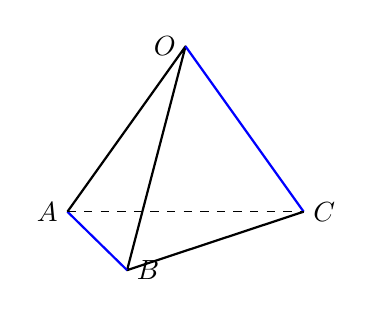
\begin{tikzpicture}[style={x={(-135:0.5)},y={(1cm,0)},z={(0,1cm)}}, line join=round, scale=3]
\coordinate[label=left: {$A$}] (A) at (0,-0.5,0);
\coordinate[label=right:{$B$}] (B) at (0.7,0,0);
\coordinate[label=right:{$C$}] (C) at (0,0.5,0);
\coordinate[label=left: {$O$}] (O) at (0,0,0.7);
\draw[thick] (A)--(O)--(B)--(C);
\draw[thick,blue] (A)--(B) (O)--(C);
\draw[dashed] (A)--(C);
\end{tikzpicture}
\end{figure}

解:
\begin{align*}
\overrightarrow{OC}\cdot \overrightarrow{AB}&=\left( \overrightarrow{AC}-\overrightarrow{AO} \right) \cdot \left( \overrightarrow{CB}-\overrightarrow{CA} \right) \\
&=\overrightarrow{AC}\cdot \overrightarrow{CB}-\overrightarrow{AO}\cdot \overrightarrow{CB}-\overrightarrow{AC}\cdot \overrightarrow{CA}+\overrightarrow{AO}\cdot \overrightarrow{CA} \\
&=\overrightarrow{AC}\cdot \overrightarrow{CB}+\overrightarrow{AC}\cdot \overrightarrow{AC}+\overrightarrow{AO}\cdot \overrightarrow{CA} \\
&=\overrightarrow{AC}\cdot \overrightarrow{AB}-\overrightarrow{AO}\cdot \overrightarrow{AC} \\
&=\overrightarrow{AC}\cdot \overrightarrow{OB}=0
\end{align*}

深入分析:

我们证明了在任意的四面体中,只要两组对棱垂直,则第三组对棱一定垂直。我们可以进一步分析,这样三组对棱垂直的情况下,四面体会有什么性质。

以$OB\bot AC$为例,意思就是$B,O$两点在$AC$上的投影重合,也即任意两个顶点在对面棱上的投影重合。根据这个结论建立如下左图的坐标系,可得:
\begin{align*}
&\because \begin{cases}
	OA\bot BC\Rightarrow \left( 0,y_A,-z_O \right) \cdot \left( -x_B,y_C,-z_B \right) =0\\
	OC\bot BA\Rightarrow \left( 0,y_C,-z_O \right) \cdot \left( -x_B,y_A,-z_B \right) =0\\
\end{cases} \\
&\therefore y_Ay_C+z_Oz_B=0
\end{align*}
四面体不一定非要正四面体,特别地,当$z_B=0$时,要么$y_A=0$要么$y_C=0$,四面体为长方体的一个角,如下右图。

\begin{figure}[h]
\centering
\begin{minipage}{.49\textwidth}
\centering
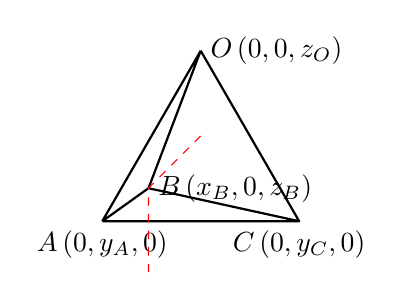
\begin{tikzpicture}[style={x={(-135:0.5)},y={(1cm,0)},z={(0,1cm)}}, line join=round, scale=2.5]
\mydrawxyz{0}{1.1}{-0.8}{0.8}{0}{1.1}
\coordinate[label=below:{$A\left( 0,y_A,0 \right) $}]   (A) at (0,-0.5,0);
\coordinate[label=below:{$C\left( 0,y_C,0 \right) $}]   (C) at (0,0.5,0);
\coordinate[label=right:{$B\left( x_B,0,z_B \right) $}] (B) at (0.75,0,0.433);
\coordinate[label=right:{$O\left( 0,0,z_O \right) $}]   (O) at (0,0,0.866);
\coordinate (Bx) at (0.75,0,0);
\coordinate (Bz) at (0,0,0.433);
\draw[thick] (O)--(A) (O)--(B) (O)--(C) (A)--(B)--(C)--(A);
\draw[dashed,red] (Bz)--(B)--(Bx);
\end{tikzpicture}
\end{minipage}
\begin{minipage}{.49\textwidth}
\centering
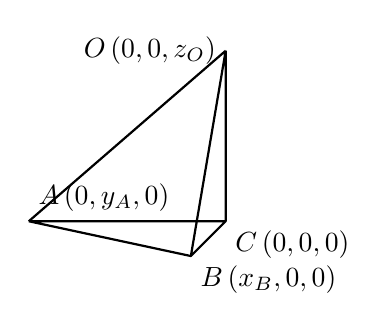
\begin{tikzpicture}[style={x={(-135:0.5)},y={(1cm,0)},z={(0,1cm)}}, line join=round, scale=2.5]
\mydrawxyz{0}{1.1}{-1.3}{0.3}{0}{1.1}
\coordinate[label=above right:{$A\left( 0,y_A,0 \right) $}] (A) at (0,-1,0);
\coordinate[label=below right:{$C\left( 0,0,0 \right) $}]   (C) at (0,0,0);
\coordinate[label=below right:{$B\left( x_B,0,0 \right) $}] (B) at (0.5,0,0);
\coordinate[label=left:       {$O\left( 0,0,z_O \right) $}] (O) at (0,0,0.866);
\draw[thick] (O)--(A) (O)--(B) (O)--(C) (A)--(B)--(C)--(A);
\end{tikzpicture}
\end{minipage}
\end{figure}

\begin{tcolorbox}
本题依然考察向量内积的几何意义。
\end{tcolorbox}

~

\begin{example}[拓广探索10,难度:$\star \star $]
如图,在四面体$OABC$中,$OA=OB,CA=CB$,$E,F,G,H$分别是$OA,OB,BC,CA$的中点。求证:四边形$EFGH$是矩形。
\end{example}

\begin{figure}[h]
\centering
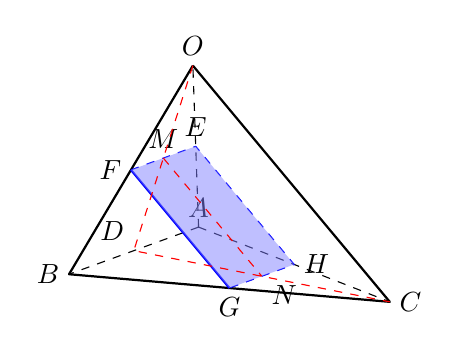
\begin{tikzpicture}[style={x={(-160:0.7)},y={(1cm,-0.2cm)},z={(0,1cm)}}, line join=round, scale=2.5]
\coordinate[label=above:      {$A$}] (A) at (-0.5,-0.3,0);
\coordinate[label=left:       {$B$}] (B) at (0.5,-0.3,0);
\coordinate[label=right:      {$C$}] (C) at (0,1,0);
\coordinate[label=above:      {$O$}] (O) at (0,0,1);
\coordinate[label=left:       {$F$}] (F) at ($(O)!0.5!(B)$);
\coordinate[label=above:      {$E$}] (E) at ($(O)!0.5!(A)$);
\coordinate[label=below:      {$G$}] (G) at ($(C)!0.5!(B)$);
\coordinate[label=right:      {$H$}] (H) at ($(C)!0.5!(A)$);
\coordinate[label=above left: {$D$}] (D) at ($(A)!0.5!(B)$);
\coordinate[label=above:      {$M$}] (M) at ($(F)!0.5!(E)$);
\coordinate[label=below right:{$N$}] (N) at ($(G)!0.5!(H)$);
\draw[thick] (O)--(B)--(C)--(O);
\draw[dashed] (A)--(O) (A)--(B) (A)--(C);
\draw[thick,blue] (F)--(G);
\draw[dashed,blue] (F)--(E)--(H)--(G);
\fill[blue!50!white,opacity=0.5] (F)--(G)--(H)--(E)--cycle;
\draw[dashed,red] (O)--(D)--(C) (M)--(N);
\end{tikzpicture}
\end{figure}

解:

首先,不难通过$\overrightarrow{FG}=\overrightarrow{EH}$证明四边形$EFGH$是平行四边形。

再证明$\angle EFG$为直角。直接用向量的方法证明$\overrightarrow{FG}\cdot \overrightarrow{FE}=0$较复杂。找到$AB$中点$D$,连接$OD,CD$,不难证明$OD,CD$是三角形的中垂线,而且$FG,MN$平行且相等,所以也即证明$\overrightarrow{MN}\cdot \overrightarrow{FE}=0$。
\[
\overrightarrow{MN}\cdot \overrightarrow{FE}=\left( \overrightarrow{DN}-\overrightarrow{DM} \right) \cdot \overrightarrow{FE}=\overrightarrow{DN}\cdot \overrightarrow{GH}-\overrightarrow{DM}\cdot \overrightarrow{FE}
\]

深入分析:

不难发现,当$AB$长度一定时,$OD,CD$决定了矩形面积,我们可以考察一下当矩形面积$S$和$DO,DC$长度的关系。
\begin{align*}
&\because S=\frac{AB}{2}\cdot \frac{OC}{2} \\
&\because \cos \angle ODC=\frac{DO^2+DC^2-OC^2}{2\cdot DO\cdot DC} \\
&\therefore S=\frac{AB}{4}\cdot \left( DO^2+DC^2-2\cos \angle ODC\cdot DO\cdot DC \right)
\end{align*}
易得:
\begin{itemize}
    \item 当$S$恒定时,$OD,CD$是一个椭圆关系,可设$\angle ODC\in \left( 0,\frac{\pi}{2} \right] $,则$2\cos \angle ODC\in \left[ 0,2 \right) $,椭圆转了45°,特别地,当$DO\bot DC$时,为圆;
    \item 当$OD,CD$相互制约时,$S$有最值。
\end{itemize}

\begin{tcolorbox}
本题需要添加辅助线,用纯几何+向量的方法,事半功倍。
\end{tcolorbox}






\newpage
\section{空间向量基本定理}

本节要点:
\begin{itemize}
    \item 掌握空间向量基本定理。
\end{itemize}

\begin{theorem}[空间向量基本定理]
设$\boldsymbol{a},\boldsymbol{b},\boldsymbol{c}$为三个不共面的空间向量,则对于任意向量$\boldsymbol{p}$,存在唯一的有序实数组$\left( x,y,z \right) $,使得
\[
\boldsymbol{p}=x\boldsymbol{a}+y\boldsymbol{b}+z\boldsymbol{c}
\]
我们把$\left\{ \boldsymbol{a},\boldsymbol{b},\boldsymbol{c} \right\} $称作空间的一个{\bf 基},把$\boldsymbol{a},\boldsymbol{b},\boldsymbol{c}$称作{\bf 基向量},对应的$\left( x,y,z \right) $称为$\boldsymbol{p}$在该组基下的{\bf 坐标}。
\end{theorem}

该定理和平面向量基本定理一样,指的是向量可以由基组合得到。也要注意,定理表达的意思是给定一个基就有一个坐标与之对应,所以不同的基有不同的坐标,但$\boldsymbol{p}$还是那个$\boldsymbol{p}$,也即:
\[
\boldsymbol{p}=x\boldsymbol{a}+y\boldsymbol{b}+z\boldsymbol{c}=l\boldsymbol{d}+m\boldsymbol{e}+n\boldsymbol{f}
\]

%============================================================
\subsection{习题}

\begin{example}[拓广探索8,难度:$\star \star $]
已知四面体中三组相对棱的中点间的距离都相等,求证:这个四面体相对的棱两两垂直。
\end{example}

解:

如下图,不难得到三组相对棱的中点连接的向量:

\begin{figure}[h]
\centering
\begin{minipage}{.32\textwidth}
\centering
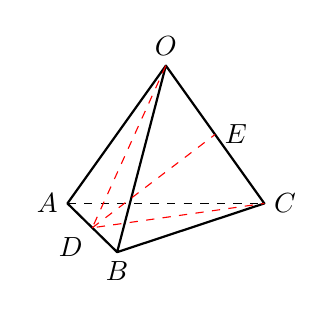
\begin{tikzpicture}[style={x={(-135:0.5)},y={(1cm,0)},z={(0,1cm)}}, line join=round, scale=2.5]
\coordinate[label=left:      {$A$}] (A) at (0,-0.5,0);
\coordinate[label=below:     {$B$}] (B) at (0.7,0,0);
\coordinate[label=right:     {$C$}] (C) at (0,0.5,0);
\coordinate[label=above:     {$O$}] (O) at (0,0,0.7);
\coordinate[label=below left:{$D$}] (D) at ($(A)!0.5!(B)$);
\coordinate[label=right:     {$E$}] (E) at ($(O)!0.5!(C)$);
\draw[thick] (B)--(O)--(A)--(B)--(C)--(O);
\draw[dashed] (A)--(C);
\draw[dashed,red] (D)--(E) (O)--(D)--(C);
\end{tikzpicture}
\end{minipage}
\begin{minipage}{.32\textwidth}
\centering
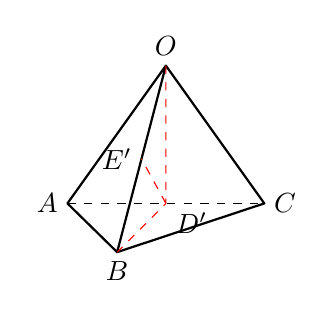
\begin{tikzpicture}[style={x={(-135:0.5)},y={(1cm,0)},z={(0,1cm)}}, line join=round, scale=2.5]
\coordinate[label=left:       {$A$}]  (A) at (0,-0.5,0);
\coordinate[label=below:      {$B$}]  (B) at (0.7,0,0);
\coordinate[label=right:      {$C$}]  (C) at (0,0.5,0);
\coordinate[label=above:      {$O$}]  (O) at (0,0,0.7);
\coordinate[label=below right:{$D'$}] (D) at ($(A)!0.5!(C)$);
\coordinate[label=left:       {$E'$}] (E) at ($(O)!0.5!(B)$);
\draw[thick] (B)--(O)--(A)--(B)--(C)--(O);
\draw[dashed] (A)--(C);
\draw[dashed,red] (D)--(E) (O)--(D)--(B);
\end{tikzpicture}
\end{minipage}
\begin{minipage}{.32\textwidth}
\centering
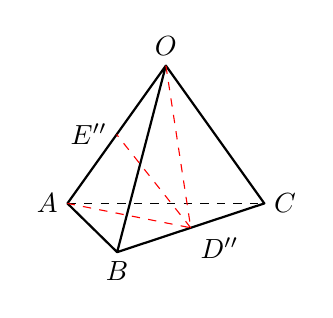
\begin{tikzpicture}[style={x={(-135:0.5)},y={(1cm,0)},z={(0,1cm)}}, line join=round, scale=2.5]
\coordinate[label=left:       {$A$}]   (A) at (0,-0.5,0);
\coordinate[label=below:      {$B$}]   (B) at (0.7,0,0);
\coordinate[label=right:      {$C$}]   (C) at (0,0.5,0);
\coordinate[label=above:      {$O$}]   (O) at (0,0,0.7);
\coordinate[label=below right:{$D''$}] (D) at ($(B)!0.5!(C)$);
\coordinate[label=left:       {$E''$}] (E) at ($(O)!0.5!(A)$);
\draw[thick] (B)--(O)--(A)--(B)--(C)--(O);
\draw[dashed] (A)--(C);
\draw[dashed,red] (D)--(E) (O)--(D)--(A);
\end{tikzpicture}
\end{minipage}
\end{figure}

\begin{align*}
&\overrightarrow{DE}=-\frac{1}{4}\left( \overrightarrow{OB}+\overrightarrow{OA}+\overrightarrow{CB}+\overrightarrow{CA} \right) \\
&\overrightarrow{D'E'}=-\frac{1}{4}\left( \overrightarrow{OA}+\overrightarrow{OC}+\overrightarrow{BA}+\overrightarrow{BC} \right) \\
&\overrightarrow{D''E''}=-\frac{1}{4}\left( \overrightarrow{AB}+\overrightarrow{AC}+\overrightarrow{OB}+\overrightarrow{OC} \right)
\end{align*}
若要平方进行长度相等,非常复杂,我们简化,使之都用$OX$表示:
\begin{align*}
&\overrightarrow{DE}=-\frac{1}{2}\left( \overrightarrow{OB}+\overrightarrow{OA}-\overrightarrow{OC} \right) \\
&\overrightarrow{D'E'}=-\frac{1}{2}\left( \overrightarrow{OA}+\overrightarrow{OC}-\overrightarrow{OB} \right) \\
&\overrightarrow{D''E''}=-\frac{1}{2}\left( \overrightarrow{OB}+\overrightarrow{OC}-\overrightarrow{OA} \right)
\end{align*}
取$\left| \overrightarrow{DE} \right|=\left| \overrightarrow{D'E'} \right|$分析:
\begin{align*}
&\because \left| \overrightarrow{DE} \right|=\left| \overrightarrow{D'E'} \right| \\
&\therefore \left( \overrightarrow{OB}+\overrightarrow{OA}-\overrightarrow{OC} \right) ^2=\left( \overrightarrow{OA}+\overrightarrow{OC}-\overrightarrow{OB} \right) ^2 \\
&\therefore \overrightarrow{OB}\cdot \overrightarrow{OA}-\overrightarrow{OA}\cdot \overrightarrow{OC}=\overrightarrow{OA}\cdot \overrightarrow{OC}-\overrightarrow{OA}\cdot \overrightarrow{OB} \\
&\therefore \overrightarrow{OB}\cdot \overrightarrow{OA}-\overrightarrow{OA}\cdot \overrightarrow{OC}=0 \\
&\therefore \overrightarrow{OA}\cdot \left( \overrightarrow{OB}-\overrightarrow{OC} \right) =0 \\
&\therefore \overrightarrow{OA}\cdot \overrightarrow{CB}=0
\end{align*}
余下略。

深入分析:

结合上一节的拓广探索9,若三对棱垂直了,计算一下对棱的中点距。

\begin{figure}[h]
\centering
\begin{minipage}{.49\textwidth}
\centering
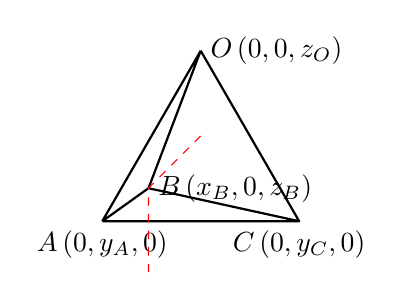
\begin{tikzpicture}[style={x={(-135:0.5)},y={(1cm,0)},z={(0,1cm)}}, line join=round, scale=2.5]
\mydrawxyz{0}{1.1}{-0.8}{0.8}{0}{1.1}
\coordinate[label=below:{$A\left( 0,y_A,0 \right) $}]   (A) at (0,-0.5,0);
\coordinate[label=below:{$C\left( 0,y_C,0 \right) $}]   (C) at (0,0.5,0);
\coordinate[label=right:{$B\left( x_B,0,z_B \right) $}] (B) at (0.75,0,0.433);
\coordinate[label=right:{$O\left( 0,0,z_O \right) $}]   (O) at (0,0,0.866);
\coordinate (Bx) at (0.75,0,0);
\coordinate (Bz) at (0,0,0.433);
\draw[thick] (O)--(A) (O)--(B) (O)--(C) (A)--(B)--(C)--(A);
\draw[dashed,red] (Bz)--(B)--(Bx);
\end{tikzpicture}
\end{minipage}
\begin{minipage}{.49\textwidth}
\centering
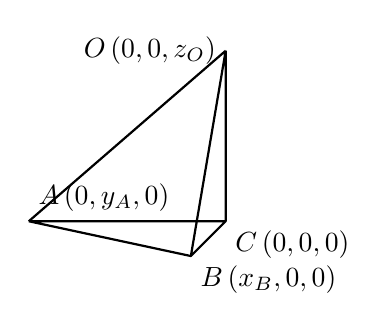
\begin{tikzpicture}[style={x={(-135:0.5)},y={(1cm,0)},z={(0,1cm)}}, line join=round, scale=2.5]
\mydrawxyz{0}{1.1}{-1.3}{0.3}{0}{1.1}
\coordinate[label=above right:{$A\left( 0,y_A,0 \right) $}] (A) at (0,-1,0);
\coordinate[label=below right:{$C\left( 0,0,0 \right) $}]   (C) at (0,0,0);
\coordinate[label=below right:{$B\left( x_B,0,0 \right) $}] (B) at (0.5,0,0);
\coordinate[label=left:       {$O\left( 0,0,z_O \right) $}] (O) at (0,0,0.866);
\draw[thick] (O)--(A) (O)--(B) (O)--(C) (A)--(B)--(C)--(A);
\end{tikzpicture}
\end{minipage}
\end{figure}

以$OA,BC$为例,它们的中点距为$\left( \frac{x_B}{2},\frac{y_A}{2},\frac{z_B}{2} \right) ,\left( 0,\frac{y_C}{2},\frac{z_O}{2} \right) $的距离,令$l$,则有:
\begin{align*}
&\because OA\bot BC\Rightarrow \left( 0,y_A,-z_O \right) \cdot \left( -x_B,y_C,-z_B \right) =0 \\
&\therefore y_Ay_C+z_Oz_B=0 \\
&\therefore l^2=\left( \frac{x_B}{2} \right) ^2+\left( \frac{y_A-y_C}{2} \right) ^2+\left( \frac{z_B-z_O}{2} \right) ^2 \\
&\therefore 4l^2={x_B}^2+{y_A}^2+{y_C}^2+{z_B}^2+{z_O}^2=OA^2+BC^2
\end{align*}
而且有:
\[
OA^2+BC^2=OC^2+AB^2=OB^2+AC^2
\]
这也是对棱垂直的四面体的性质,不难发现,正四面体和长方体一角都是该式的特殊形式。

\begin{tcolorbox}
本题思路简单,从定义出发,但是计算量大,如果不将一开始的表达式化简,几乎无解。
\end{tcolorbox}






\newpage
\section{空间向量及其运算的坐标表示}

本节要点:
\begin{itemize}
    \item 掌握向量运算的坐标表示。
\end{itemize}

%============================================================
\subsection{空间直角坐标系}

和平面向量一样,当我们定义了空间直角坐标系后,可以得到空间向量的3个等价表示方法:
\begin{itemize}
    \item $\overrightarrow{AB}$:表示三维空间的有向线段;
    \item $x\boldsymbol{i}+y\boldsymbol{j}+z\boldsymbol{k}$:表示{\it xyz}坐标系中的有向线段;
    \item $\left( x,y,z \right) $:表示{\it xyz}坐标系中的点。
\end{itemize}

\begin{tcolorbox}
这里要注意一点,直角坐标系的右手性是人为规定的。
\end{tcolorbox}

%============================================================
\subsection{空间向量运算的坐标系表示}

加法、数乘、内积的坐标表示如下:
\begin{align*}
&\boldsymbol{a}+\boldsymbol{b}=\left( x_{\boldsymbol{a}}+x_{\boldsymbol{b}} \right) \boldsymbol{i}+\left( y_{\boldsymbol{a}}+y_{\boldsymbol{b}} \right) \boldsymbol{j}+\left( z_{\boldsymbol{a}}+z_{\boldsymbol{b}} \right) \boldsymbol{k} \\
&\lambda \boldsymbol{a}=\lambda x_{\boldsymbol{a}}\boldsymbol{i}+\lambda y_{\boldsymbol{a}}\boldsymbol{j}+\lambda z_{\boldsymbol{a}}\boldsymbol{k} \\
&\boldsymbol{a}\cdot \boldsymbol{b}=x_{\boldsymbol{a}}\cdot x_{\boldsymbol{b}}+y_{\boldsymbol{a}}\cdot y_{\boldsymbol{b}}+z_{\boldsymbol{a}}\cdot z_{\boldsymbol{b}}=\left| \boldsymbol{a} \right|\left| \boldsymbol{b} \right|\cos \alpha
\end{align*}

%============================================================
\subsection{习题}

\begin{example}[拓广探索9,难度:$\star \star $]
$\left\{ \boldsymbol{a},\boldsymbol{b},\boldsymbol{c} \right\} $是空间的一个单位正交基底,向量$\boldsymbol{p}=\boldsymbol{a}+2\boldsymbol{b}+3\boldsymbol{c}$,$\left\{ \boldsymbol{a}+\boldsymbol{b},\boldsymbol{a}-\boldsymbol{b},\boldsymbol{c} \right\} $是空间的另一个基底,用$\left\{ \boldsymbol{a}+\boldsymbol{b},\boldsymbol{a}-\boldsymbol{b},\boldsymbol{c} \right\} $表示向量$\boldsymbol{p}$。
\end{example}

解:

$\boldsymbol{p}$在新坐标系下可表示为:
\[
\boldsymbol{p}=x\left( \boldsymbol{a}+\boldsymbol{b} \right) +y\left( \boldsymbol{a}-\boldsymbol{b} \right) +z\boldsymbol{c}=\left( x+y \right) \boldsymbol{a}+\left( x-y \right) \boldsymbol{b}+z\boldsymbol{c}
\]
于是:
\begin{align*}
&\begin{cases}
	x+y=1\\
	x-y=2\\
	z=3\\
\end{cases}\Rightarrow \begin{cases}
	x=\frac{3}{2}\\
	y=-\frac{1}{2}\\
	z=3\\
\end{cases} \\
&\boldsymbol{p}=\frac{3}{2}\left( \boldsymbol{a}+\boldsymbol{b} \right) -\frac{1}{2}\left( \boldsymbol{a}-\boldsymbol{b} \right) +3\boldsymbol{c}
\end{align*}

\begin{tcolorbox}
本题其实是对空间向量基本定理的拓展,任意向量在不同基下有不同的表示,但向量还是那个向量。
\end{tcolorbox}






\newpage
\section{空间向量的应用}

本节要点:
\begin{itemize}
    \item 掌握空间点线面的方程;
    \item 熟练掌握使用向量判断空间点线面的关系。
\end{itemize}

%============================================================
\subsection{用空间向量研究直线、平面的位置关系}

首先定义点、线、面的向量表达式。

{\bf 空间中的点}

直接用向量或其坐标表示:
\[
\overrightarrow{OP} \qquad \boldsymbol{p} \qquad \left( x_{\boldsymbol{p}},y_{\boldsymbol{p}},z_{\boldsymbol{p}} \right)
\]

{\bf 空间中的直线}

直线的定义是和给定点$P_0$构成的向量与给定向量$\boldsymbol{n}$平行的所有点的集合,即:
\[
\overrightarrow{P_0P}=\lambda \boldsymbol{n} \quad \text{或} \quad \left( x-x_0,y-y_0,z-z_0 \right) =\lambda \left( A,B,C \right)
\]
展开后得空间直线方程:
\[
\frac{x-x_0}{A}=\frac{y-y_0}{B}=\frac{z-z_0}{C}
\]
其中:
\begin{itemize}
    \item $\boldsymbol{n}=\left( A,B,C \right) $:直线的方向;
    \item $\left( x_0,y_0,z_0 \right) $:直线上一点$P_0$的坐标。
\end{itemize}

{\bf 空间中的平面}

平面的定义是和给定点$P_0$构成的向量与给定向量$\boldsymbol{n}$垂直得所有点得集合,即:
\[
\overrightarrow{P_0P}\cdot \boldsymbol{n}=0 \quad \text{或} \quad A\left( x-x_0 \right) +B\left( y-y_0 \right) +C\left( z-z_0 \right) =0
\]
展开后得到空间平面的一般方程:
\[
Ax+By+Cz+D=0
\]
其中:
\begin{itemize}
    \item $\boldsymbol{n}=\left( A,B,C \right) $:平面的法线方向;
    \item $\left( x_0,y_0,z_0 \right) $:平面上一点$P_0$的坐标。
\end{itemize}
特别地,当平面和{\it xyz}轴分别交于$x_0,y_0,z_0$时,则可以写成截距式:
\[
\frac{x}{x_0}+\frac{y}{y_0}+\frac{z}{z_0}=0
\]

\begin{tcolorbox}
以上定义中,关键在于点和方向。点好理解,直线或平面上的点,直线的方向也好理解,面的方向是第一次碰到,我们取平面的法线的方向作为平面的方向。还要注意,高中阶段的方向,不分正反!
\end{tcolorbox}

\begin{theorem}
根据以上定义,我们不难得到直线和平面关系的判定定理:
\begin{itemize}
    \item 若$\boldsymbol{l}_1=\lambda \boldsymbol{l}_2$,则两直线$l_1,l_2$平行;
    \item 若$\boldsymbol{l}\cdot \boldsymbol{n}=0$,则直线$l$平面$\alpha $平行;
    \item 若$\boldsymbol{n}_{\alpha}=\lambda \boldsymbol{n}_{\beta}$,则两平面$\alpha ,\beta $平行;
    \item 若$\boldsymbol{l}_1\cdot \boldsymbol{l}_2=0$,则两直线$l_1,l_2$垂直;
    \item 若$\boldsymbol{l}=\lambda \boldsymbol{n}$,则直线$l$平面$\alpha $垂直;
    \item 若$\boldsymbol{n}_{\alpha}\cdot \boldsymbol{n}_{\beta}=0$,则两平面$\alpha ,\beta $垂直。
\end{itemize}
\end{theorem}

\begin{table}[h]
\centering
\begin{tabular}{ccc}
    \toprule
     & 平行 & 垂直\\
    \midrule
    线线$l_1,l_2$ & $\boldsymbol{l}_1=\lambda \boldsymbol{l}_2$ & $\boldsymbol{l}_1\cdot \boldsymbol{l}_2=0$\\
    线面$l,\alpha $ & $\boldsymbol{l}\cdot \boldsymbol{n}=0$ & $\boldsymbol{l}=\lambda \boldsymbol{n}$\\
    面面$\alpha ,\beta $ & $\boldsymbol{n}_{\alpha}=\lambda \boldsymbol{n}_{\beta}$ & $\boldsymbol{n}_{\alpha}\cdot \boldsymbol{n}_{\beta}=0$\\
    \bottomrule
\end{tabular}
\end{table}

%============================================================
\subsection{用空间向量研究距离、夹角问题}

如下图,点$P$到直线和平面的距离表达式:

\begin{figure}[h]
\centering
\begin{minipage}{.49\textwidth}
\centering
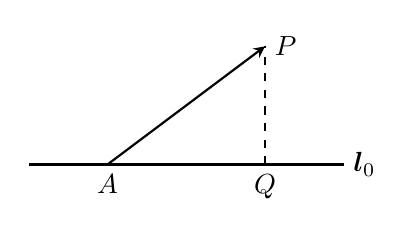
\begin{tikzpicture}[line join=round, scale=0.5]
\coordinate[label=below:{$A$}]                (A)  at (0,0);
\coordinate[label=below:{$Q$}]                (Q)  at (4,0);
\coordinate[label=right:{$P$}]                (P)  at (4,3);
\coordinate[label=right:{$\boldsymbol{l}_0$}] (l0) at (6,0);
\draw[thick] ($(A)!-0.5!(Q)$)--($(A)!1.5!(Q)$);
\draw[thick,-stealth] (A)--(P);
\draw[dashed] (Q)--(P);
\end{tikzpicture}
\end{minipage}
\begin{minipage}{.49\textwidth}
\centering
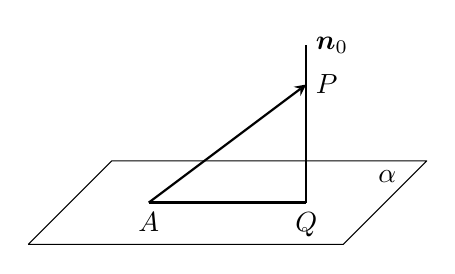
\begin{tikzpicture}[style={x={(-135:0.5)},y={(1cm,0)},z={(0,1cm)}}, line join=round, scale=0.5]
\draw (3,-2,0)--(3,6,0)--(-3,6,0)--(-3,-2,0)--(3,-2,0);
\coordinate[label=below:{$\alpha $}]          (a)  at (-3,5,0);
\coordinate[label=below:{$A$}]                (A)  at (0,0,0);
\coordinate[label=below:{$Q$}]                (Q)  at (0,4,0);
\coordinate[label=right:{$P$}]                (P)  at (0,4,3);
\coordinate[label=right:{$\boldsymbol{n}_0$}] (n0) at (0,4,4);
\draw[thick] (A)--(Q);
\draw[thick,-stealth] (A)--(P);
\draw[thick] (Q)--(n0);
\end{tikzpicture}
\end{minipage}
\end{figure}

\[
PQ=\sqrt{\overrightarrow{AP}^2-\left( \overrightarrow{AP}\cdot \boldsymbol{l}_0 \right) ^2} \qquad \qquad PQ=\left| \overrightarrow{AP}\cdot \boldsymbol{n}_0 \right|
\]
其中:
\begin{itemize}
    \item $\boldsymbol{l}_0$:直线的单位方向向量;
    \item $\boldsymbol{n}_0$:平面的单位法向方向向量。
\end{itemize}

~

如下图,线线、线面、面面夹角的余弦表达式:
\[
\cos \theta =\frac{\left| \boldsymbol{l}_1\cdot \boldsymbol{l}_2 \right|}{\left| \boldsymbol{l}_1 \right|\left| \boldsymbol{l}_2 \right|} \qquad \sin \theta =\frac{\left| \boldsymbol{l}\cdot \boldsymbol{n} \right|}{\left| \boldsymbol{l} \right|\left| \boldsymbol{n} \right|} \qquad \cos \theta =\frac{\left| \boldsymbol{n}_1\cdot \boldsymbol{n}_2 \right|}{\left| \boldsymbol{n}_1 \right|\left| \boldsymbol{n}_2 \right|}
\]

\begin{figure}[h]
\centering
\begin{minipage}{.32\textwidth}
\centering
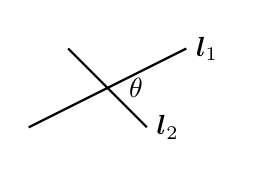
\begin{tikzpicture}[line join=round, scale=0.5]
\coordinate                                   (l11) at (-2,-1);
\coordinate[label=right:{$\boldsymbol{l}_1$}] (l12) at (2,1);
\coordinate                                   (l21) at (-1,1);
\coordinate[label=right:{$\boldsymbol{l}_2$}] (l22) at (1,-1);
\coordinate[label=right:{$\theta $}]          (t)   at (0.3,0);
\draw[thick] (l11)--(l12) (l21)--(l22);
\end{tikzpicture}
\end{minipage}
\begin{minipage}{.32\textwidth}
\centering
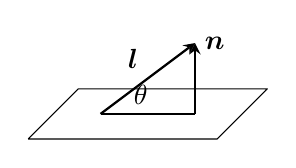
\begin{tikzpicture}[style={x={(-135:0.5)},y={(1cm,0)},z={(0,1cm)}}, line join=round, scale=0.3]
\draw (3,-2,0)--(3,6,0)--(-3,6,0)--(-3,-2,0)--(3,-2,0);
\coordinate                                       (A) at (0,0,0);
\coordinate                                       (Q) at (0,4,0);
\coordinate                                       (P) at (0,4,3);
\coordinate[label=above left: {$\boldsymbol{l}$}] (l) at ($(A)!0.5!(P)$);
\coordinate[label=right:      {$\boldsymbol{n}$}] (n) at (P);
\coordinate[label=above right:{$\theta $}]        (t) at (0,1,0);
\draw[thick] (A)--(Q);
\draw[thick,-stealth] (A)--(P);
\draw[thick,-stealth] (Q)--(P);
\end{tikzpicture}
\end{minipage}
\begin{minipage}{.32\textwidth}
\centering
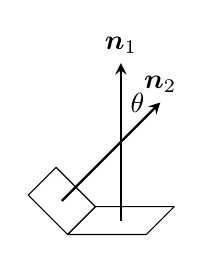
\begin{tikzpicture}[style={x={(-135:0.5)},y={(1cm,0)},z={(0,1cm)}}, line join=round, scale=0.5]
\draw (1,2,0)--(1,0,0)--(-1,0,0)--(-1,2,0)--(1,2,0);
\draw (1,0,0)--(1,-1,1)--(-1,-1,1)--(-1,0,0)--(1,0,0);
\coordinate[label=above:      {$\boldsymbol{n}_1$}] (n1) at (0,1,4);
\coordinate[label=above:      {$\boldsymbol{n}_2$}] (n2) at (0,2,3);
\coordinate[label=above right:{$\theta $}]          (t)  at (0,1,2.5);
\draw[thick,-stealth] (0,1,0)--(n1);
\draw[thick,-stealth] (0,-0.5,0.5)--(n2);
\end{tikzpicture}
\end{minipage}
\end{figure}

\begin{tcolorbox}
本节的例1、例2、例3、例9、例10,都值得反复阅读。
\end{tcolorbox}

%============================================================
\subsection{习题}

\begin{example}[拓广探索18,难度:$\star \star \star $]
在如图所示的实验装置中,两个正方形框架$ABCD$,$ABEF$的边长都是1,且它们所在的平面互相垂直。活动弹子$M,N$分别在正方形对角线$AC$和$BF$上移动,且$CM$和$BN$的长度保持相等,记$CM=BN=a,0<a<\sqrt{2}$。
\begin{enumerate}
    \item 求$MN$的长;
    \item $a$为何值时,$MN$的长最小?
    \item 当$MN$的长最小时,求平面$MNA$和$MNB$夹角的余弦值。
\end{enumerate}
\end{example}

\begin{figure}[h]
\centering
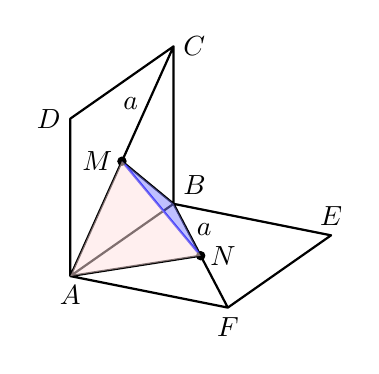
\begin{tikzpicture}[style={x={(-145:0.8)},y={(1cm,-0.2cm)},z={(0,1cm)}}, line join=round, scale=2]
\pgfmathparse{0.6/2}
\mydrawxyz{0}{1.4}{0}{1.4}{0}{1.4}
\coordinate[label=above right:{$B$}] (B) at (0,0,0);
\coordinate[label=below:      {$A$}] (A) at (1,0,0);
\coordinate[label=right:      {$C$}] (C) at (0,0,1);
\coordinate[label=left:       {$D$}] (D) at (1,0,1);
\coordinate[label=above:      {$E$}] (E) at (0,1,0);
\coordinate[label=below:      {$F$}] (F) at (1,1,0);
\coordinate[label=left:       {$M$}] (M) at ($(A)!0.5!(C)$);
\coordinate[label=right:      {$N$}] (N) at ($(B)!0.5!(F)$);
\coordinate[label=left:       {$a$}] (a) at ($(C)!0.5!(M)$);
\coordinate[label=right:      {$a$}] (a) at ($(B)!0.5!(N)$);
\draw[thick] (A)--(B)--(C)--(D)--(A)--(C) (F)--(B)--(E)--(F)--(A) (A)--(N) (B)--(M);
\draw[thick,blue] (M)--(N);
\fill (M) circle (\pgfmathresult mm);
\fill (N) circle (\pgfmathresult mm);
\fill[blue!50!white,opacity=0.5] (M)--(N)--(B)--cycle;
\fill[pink!50!white,opacity=0.5] (M)--(N)--(A)--cycle;
\end{tikzpicture}
\end{figure}

解:

(1)以$B$为原点建立直角坐标系。根据关系可得$M,N$坐标$M=\left( x,0,1-x \right) ,N=\left( x,x,0 \right) $,其中$\sqrt{2}x=a$,于是:
\[
MN=\sqrt{x^2+\left( 1-x \right) ^2}=\sqrt{2x^2-2x+1}=\sqrt{\left( \sqrt{2}x-\frac{1}{\sqrt{2}} \right) ^2+\frac{1}{2}}
\]

(2)可见,当$x=\frac{1}{2}$时,$MN$最小,为$\sqrt{\frac{1}{2}}$,此时$a=\frac{\sqrt{2}}{2}$。

(3)不难发现$\bigtriangleup AMN,\bigtriangleup BMN$均为等边三角形,后略。

深入分析:

探讨一下$MN$最值。首先有一个直觉,高中阶段的不等值最终都可以归结为基本不等式,$MN$两头都是$CB=AF=1$,一定是对称点取到最值,事实也是如此。另一个直觉,异面直线距离最短,$MN$应该是距离,但显然结果的$MN$并不是距离,这点从$MN$和$AC,BF$都不垂直可以得出。两个直觉发生矛盾了。

假设$M,N$各自运动,我们看看什么时候$MN$最短。
另$M,N$坐标$M=\left( x_m,0,1-x_m \right) ,N=\left( x_n,x_n,0 \right) $,于是:
\begin{align*}
MN&=\sqrt{\left( x_m-x_n \right) ^2+{x_n}^2+\left( 1-x_m \right) ^2} \\
&=\sqrt{2{x_m}^2-2x_mx_n+2{x_n}^2+1-2x_m}
\end{align*}
另$y=2{x_m}^2-2x_mx_n+2{x_n}^2+1-2x_m$,计算一阶和二阶偏导:
\begin{align*}
&\because \begin{cases}
	\frac{\partial y}{\partial x_m}=4x_m-2x_n-2=0\\
	\frac{\partial y}{\partial x_n}=-2x_m+4x_n=0\\
\end{cases} \quad \begin{cases}
	A=\frac{\partial ^2y}{{\partial x_m}^2}=4\\
	C=\frac{\partial ^2y}{{\partial x_n}^2}=4\\
	B=\frac{\partial ^2y}{\partial x_m\partial x_n}=-2\\
\end{cases} \\
&\therefore x_m=\frac{2}{3},x_n=\frac{1}{3}
\end{align*}
由于$AC>B,A>0$,所以该值为最小值,此时:
\begin{align*}
&M=\left( \frac{2}{3},0,\frac{1}{3} \right) ,N=\left( \frac{1}{3},\frac{1}{3},0 \right) \\
&MN=\sqrt{\left( 1/3 \right) ^2+\left( 1/3 \right) ^2+\left( 1/3 \right) ^2}=1/\sqrt{3}
\end{align*}
再考察$\bigtriangleup AMN$:
\begin{align*}
&A=\left( 1,0,0 \right) \\
&AM=\sqrt{\left( 1/3 \right) ^2+\left( 1/3 \right) ^2}=\sqrt{2}/\sqrt{3} \\
&AN=\sqrt{\left( 2/3 \right) ^2+\left( 1/3 \right) ^2}=\sqrt{5}/\sqrt{3}
\end{align*}
可见$\bigtriangleup AMN$为直角三角形,同理$\bigtriangleup BMN$也为直角三角形,此刻$MN$垂直于$AC,BF$,$MN$确实是距离。

分析可得,这两个直觉的矛盾在于$M,N$两点的运动方式,若无约束确实可以取到距离,但题目对它们的运动方式有了约束,所以取不到距离。

\begin{tcolorbox}
本题采用向量的方法将几何问题转化为代数问题,需要将几何和代数融会贯通,但总体上思路还是明确的。
\end{tcolorbox}






\newpage
\section{本章小结}

引入向量后,所有的几何问题都有了明显的思路,只是计算量大小的问题。任何几何问题采用暴力计算的方法一定能求解,但这显然不是高效的方法。要学好几何,则不可偏用向量,适当结合一定的纯几何可大大降低计算量。

%============================================================
\subsection{习题}

\begin{example}[拓广探索16,难度:$\star \star $]
如图,在棱长为$a$的正方体$OABC-O'A'B'C'$中,$E,F$分别是棱$AB,BC$上的动点,且$AE=BF$。
\begin{itemize}
    \item 求证:$A'F\bot C'E$;
    \item 当三棱锥$B'-BEF$的体积取得最大值时,求平面$B'EF$与平面$BEF$夹角的正切值。
\end{itemize}
\end{example}

\begin{figure}[h]
\centering
\begin{tikzpicture}[style={x={(-145:0.5)},y={(1cm,0)},z={(0,1cm)}}, line join=round, scale=2]
\mydrawcube[1]{O}{A}{B}{C}{O'}{A'}{B'}{C'}
\coordinate[label=below left: {$F$}] (F) at ($(B)!0.7!(C)$);
\coordinate[label=below:      {$E$}] (E) at ($(A)!0.7!(B)$);
\coordinate[label=above:      {$y$}] (y) at ($(C)!0.5!(F)$);
\coordinate[label=below right:{$x$}] (x) at ($(B)!0.5!(E)$);
\draw[dashed] (C')--(C) (O)--(C)--(B) (B')--(F)--(E);
\draw[thick] (B')--(E);
\draw[dashed,blue] (C')--(E) (A')--(F);
\fill[pink!70!white,opacity=0.5] (F)--(E)--(B)--cycle;
\fill[blue!50!white,opacity=0.5] (F)--(E)--(B')--cycle;
\end{tikzpicture}
\end{figure}

解:

(1)在$E,F$均是动点的前提下,显然不能用纯几何的方法求证。考虑采用向量的方法,以$O$为原点建立直角坐标系,于是:
\begin{align*}
&\because \begin{cases}
	F=\left( 0,y,0 \right) ,E=\left( x,a,0 \right)\\
	A'=\left( a,a,a \right) ,C'=\left( 0,0,a \right)\\
\end{cases} \\
&\therefore \begin{cases}
	\overrightarrow{A'F}=\left( -a,y-a,-a \right)\\
	\overrightarrow{C'E}=\left( x,a,-a \right)\\
\end{cases} \\
&\therefore \overrightarrow{A'F}\cdot \overrightarrow{C'E}=-ax+a\left( y-a \right) +a^2=-ax+ay \\
&\because AE=BF \\
&\therefore EB=CF \\
&\therefore x=y \\
&\therefore \overrightarrow{A'F}\cdot \overrightarrow{C'E}=0
\end{align*}

(2)三棱锥$B'-BEF$的体积
\[
V_{B'-BEF}=\frac{1}{3}\cdot S_{\bigtriangleup BEF}\cdot BB'
\]
显然当$S_{\bigtriangleup BEF}$最大时,$V_{B'-BEF}$最大,于是:
\begin{align*}
&\because S_{\bigtriangleup BEF}=\frac{1}{2}\cdot BF\cdot BE=\frac{1}{2}\cdot \left( a-y \right) \cdot x\\
&\because x=y \\
&\therefore S_{\bigtriangleup BEF}=\frac{1}{2}\left( -x^2+ax \right) \quad x\in \left( 0,a \right)
\end{align*}
显然当$x=y=1/2$时,$V_{B'-BEF}$最大,此时,$B'EF$和$BEF$均为等腰三角形,后略。

深入分析:

有兴趣可以计算一下$V_{E-FA'B'}$,提示$V_{E-FA'B'}=V_{B-FA'B'}$。再看一下$V_{E-FA'B'}$什么时候取得最大值。

\begin{tcolorbox}
该题是典型的通过向量联系几何和代数的题目,整体思路还是明显的,通过向量将几何问题转化为代数问题,剩下的就是函数了。
\end{tcolorbox}










\chapter{直线和圆的方程}

本章介绍直线和圆的方程,并讨论其位置关系。

本章要点:
\begin{itemize}
    \item 直线和圆。
    \item 位置关系。
\end{itemize}

\newpage
\section{直线的倾斜角与斜率}

本节要点:
\begin{itemize}
    \item 掌握倾斜角的概念;
    \item 掌握斜率的概念。
\end{itemize}

%============================================================
\subsection{倾斜角和斜率}

\begin{definition}[倾斜角和斜率]
我们将直线$l$的向上的方向和{\it x}轴正向所成的角称为{\bf 倾斜角},通常用希腊字母表示,不难得到$\alpha \in \left[ 0,\pi \right) $。我们称倾斜角的正切值为该斜线的{\bf 斜率},通常记作$k$,即:
\[
k:=\tan \alpha
\]
\end{definition}

\begin{tcolorbox}
注意,垂直于{\it x}轴的直线是没有斜率的。
\end{tcolorbox}

\begin{tcolorbox}
想两个问题。首先,既然有了倾斜角,为什么还要定义斜率?其次,既然要定义斜率,为什么要用正切值?用正弦或余弦不行吗?何况正弦和余弦在$\alpha \in \left[ 0,\pi \right) $上都有定义,不会像正切一样存在不定义点。XML。
\end{tcolorbox}

%============================================================
\subsection{两条直线平行和垂直的判定}

\begin{theorem}
设直线$l_1,l_2$的斜率为$k_1,k_2$,则有:
\begin{align*}
&l_1\parallel l_2\Leftrightarrow k_1=k_2 \\
&l_1\bot l_2\Leftrightarrow k_1k_2=-1
\end{align*}
\end{theorem}

\begin{tcolorbox}
注意,各自平行于两个轴的直线是没有办法用上述定理判断垂直的。
\end{tcolorbox}






\newpage
\section{直线的方程}

本节要点:
\begin{itemize}
    \item 掌握5种直线的代数形式;
    \item 深刻理解它们代表的几何意义。
\end{itemize}

~

{\bf 点斜式},$k$必须有定义,即不能垂直于{\it x}轴:
\[
y-y_0=k\left( x-x_0 \right)
\]

{\bf 斜截式},$k$必须有定义,即不能垂直于{\it x}轴:
\[
y=kx+b
\]

{\bf 两点式},对两点有要求$x_1\ne x_2$且$y_1\ne y_2$:
\[
\frac{y-y_1}{y_2-y_1}=\frac{x-x_1}{x_1-x_2}
\]

{\bf 截距式},任意一个截距都不能为0:
\[
\frac{x}{a}+\frac{y}{b}=1
\]

{\bf 一般式},任何情况都能用:
\[
Ax+By+C=0
\]

%============================================================
\subsection{拓展讨论:直线的定义}

其实我们可以参考上一章中对空间直线的描述,定义平面上的直线。

\begin{definition}[直线]
若二维平面中有一个给定点$P_0$和一个给定的向量$\boldsymbol{n}$,若平面上的点和$P_0$构成的向量与$\boldsymbol{n}$平行,则称这些点组成的集合为{\bf 直线},常用$l$表示,即:
\[
l:=\left\{ P \middle| \overrightarrow{P_0P}=\lambda \boldsymbol{n} \right\}
\]
若令$P=\left( x,y \right) ,P_0=\left( x_0,y_0 \right) ,n=A\boldsymbol{x}+B\boldsymbol{y}$,则直线可以表示为下列的{\bf 向量方程}:
\[
\left( x-x_0,y-y_0 \right) =\lambda \left( A,B \right)
\]
若保留$\lambda $,可得到{\bf 参数方程}:
\[
\begin{cases}
	x=\lambda A+x_0\\
	y=\lambda A+y_0\\
\end{cases} \quad \lambda \in \mathbb{R}
\]
若约去$\lambda $,则可得到一般式:
\begin{align*}
&\frac{x-x_0}{A}=\frac{y-y_0}{B} \\
&\left( -Bx \right) +\left( Ay \right) +\left( Bx_0-Ay_0 \right) =0
\end{align*}
\end{definition}

%============================================================
\subsection{习题}

\begin{example}[综合运用12,难度:$\star $]
若直线$l$沿{\it x}轴向左平移3个单位长度,再沿{\it y}轴向上平移1个单位长度后,回到原来的位置,试求直线$l$的斜率。
\end{example}

解一:

从定义出发,设直线$y-y_0=k\left( x-x_0 \right) $,有:
\begin{align*}
&\because y-y_0-1=k\left( x-x_0+3 \right) \\
&\therefore y-y_0-1=k\left( x-x_0 \right) +3k \\
&\therefore k=-\frac{1}{3}
\end{align*}

解二:

从向量的角度,设点直线上的点$\left( x_0,y_0 \right) $,平移后到达$\left( x_0-3,y_0+1 \right) $,又这两点都在直线上,于是:
\[
\frac{\left( y_0+1 \right) -y_0}{\left( x_0-3 \right) -x_0}=k
\]

\begin{tcolorbox}
本题考察斜率的定义。
\end{tcolorbox}






\newpage
\section{直线的交点坐标与距离公式}

本节要点:
\begin{itemize}
    \item 从二元一次方程组的解出发理解直线的几何关系;
    \item 熟练掌握点到直线的距离公式;
    \item 掌握平行线间的距离公式。
\end{itemize}

~

点线距离公式:
\[
d=\frac{\left| Ax_0+By_0+C \right|}{\sqrt{A^2+B^2}}
\]

线线距离公式:
\[
d=\frac{\left| C_1-C_2 \right|}{\sqrt{A^2+B^2}}
\]

\begin{tcolorbox}
仔细阅读距离公式的推导过程。
\end{tcolorbox}

%============================================================
\subsection{习题}

\begin{example}[综合运用14,难度:$\star $]
已知$A\left( -3,-4 \right) ,B\left( 6,3 \right) $两点到直线$l:ax+y+1=0$的距离相等,求$a$的值。
\end{example}

解一:

根据点线距离公式:
\begin{align*}
&\because d_A=\frac{\left| -3a-4+1 \right|}{\sqrt{a^2+1}} \\
&\because d_B=\frac{\left| Ax_0+By_0+C \right|}{\sqrt{A^2+B^2}}=\frac{\left| 6a+3+1 \right|}{\sqrt{a^2+1}} \\
&\because \left( -3a-3 \right) ^2=\left( 6a+4 \right) ^2 \\
&\therefore 27a^2+30a+7=0 \\
&\therefore a=-\frac{1}{3}\mathrm{or}-\frac{7}{9}
\end{align*}

解二:

根据几何关系,若两点不在同一侧,则线段$AB$的中点$\left( \frac{3}{2},-\frac{1}{2} \right) $在直线上,带入直线方程易得:
\[
a=-\frac{1}{3}
\]
或者两点在同侧,易得向量$\overrightarrow{AB}=\left( 9,7 \right) $和直线平行,于是:
\[
k=-a=\frac{7}{9}
\]

\begin{tcolorbox}
观察几何关系可以降低计算量。
\end{tcolorbox}

~

\begin{example}[拓广探索11,难度:$\star \star $]
已知$0<x<1,0<y<1$。
\begin{enumerate}
    \item 求证:$\sqrt{x^2+y^2}+\sqrt{x^2+\left( 1-y \right) ^2}+\sqrt{\left( 1-x \right) ^2+y^2}$
    
    $+\sqrt{\left( 1-x \right) ^2+\left( 1-y \right) ^2}\geqslant 2\sqrt{2}$,并求使等式成立的条件。
    \item 说明上述不等式的几何意义。
\end{enumerate}
\end{example}

解:

构建如下单位正方形$OABC$,$P$在正方形内部。

\begin{figure}[h]
\centering
\begin{tikzpicture}[line join=round, scale=2]
\mydrawxy{0}{1.3}{0}{1.2}
\mydrawsquare[1]{O}{A}{B}{C}
\draw[dashed] (A)--(C) (B)--(O);
\coordinate[label=left:{$P$}] (P) at (0.3,0.5);
\draw[dashed,blue] (C)--(P)--(A) (O)--(P)--(B);
\end{tikzpicture}
\end{figure}

根据三角形三边长度关系易得:
\begin{itemize}
    \item $\sqrt{x^2+y^2}+\sqrt{\left( 1-x \right) ^2+\left( 1-y \right) ^2}\geqslant \sqrt{2}$,当且仅当$P$在直线$OB$上时等号成立;
    \item $\sqrt{x^2+\left( 1-y \right) ^2}+\sqrt{\left( 1-x \right) ^2+y^2}\geqslant \sqrt{2}$,当且仅当$P$在直线$AC$上时等号成立;
\end{itemize}
所以,当且仅当$P$在$OB,AC$的交点时求证的等式的等号成立。

\begin{tcolorbox}
使用几何可以非常容易证明此题。
\end{tcolorbox}






\newpage
\section{圆的方程}

本节要点:
\begin{itemize}
    \item 掌握2种圆的代数形式;
    \item 深刻理解它们代表的几何意义。
\end{itemize}

~

{\bf 标准方程}:
\[
\left( x-a \right) ^2+\left( y-b \right) ^2=r^2
\]

{\bf 一般方程}:
\[
x^2+y^2+Dx+Ey+F=0
\]

\begin{tcolorbox}
详细阅读所有例题。例2和例4都是已知求三角形的外接圆,分别用标准方程和一般方程,体会两者的计算量。例5中$M$是中点,若$M$不是中点,而是某个等比例点,则$M$的运动轨迹是什么样子?再如果$A$是任意轨迹,则$M$的运动轨迹和$A$的轨迹有什么关系?早期钟表内部的细小零件的制作就是依据这个原理,XML。
\end{tcolorbox}

%============================================================
\subsection{拓展讨论:圆的定义}

我们给出圆的定义,然后推导圆的公式。

\begin{definition}[圆]
设二维平面中有一定点$P_0$,若平面上的点和$P_0$的距离都是$r>0$,则称这些点组成的集合为{\bf 圆},常用$C$表示,即:
\[
C:=\left\{ P \middle| \left| \overrightarrow{P_0P} \right|=r \right\}
\]
若令$P=\left( x,y \right) ,P_0=\left( x_0,y_0 \right) $,则圆可以表示为下列的{\bf 向量方程}:
\[
\left( x-x_0 \right) ^2+\left( y-y_0 \right) ^2=r^2
\]
使用复数的概念,可得到{\bf 参数方程}:
\[
\begin{cases}
	x-x_0=r\cos \theta\\
	y-y_0=r\sin \theta\\
\end{cases} \quad \theta \in \left[ 0,2\pi \right)
\]
\end{definition}

再考虑一个问题,考察课本给出的圆的一般方程
\[
x^2+y^2+Dx+Ey+F=0
\]
$A,B,C$去哪里了?

事实上,关于$x,y$的二次曲线,更一般的应该是:
\[
Ax^2+By^2+Cxy+Dx+Ey+F=0
\]
是一个倾斜的椭圆,当$C=0$时,椭圆归正,即长短轴平行于{it xy}轴,进一步地,当$A=B$时,为圆。

%============================================================
\subsection{习题}

\begin{example}[综合运用5,难度:$\star \star $]
已知圆的一条直径的端点分别是$A\left( x_1,y_1 \right) $,$B\left( x_2,y_2 \right) $,求证此圆的方程是
\[
\left( x-x_1 \right) \left( x-x_2 \right) +\left( y-y_1 \right) \left( y-y_2 \right) =0
\]
\end{example}

解:

用向量的方法,向量表示的点在圆上,则构成直角三角形,两个直角边的内积为0。

\begin{tcolorbox}
本题联合向量内积的几何意义,一句话就能证明,非常容易。
\end{tcolorbox}

~

\begin{example}[综合运用7,难度:$\star $]
已知等腰三角形$ABC$的一个顶点为$A\left( 4,2 \right) $,底边的一个端点为$B\left( 3,5 \right) $,求底边的另一个端点$C$的轨迹方程,并说明它是什么图形。
\end{example}

解:

显然$AB=AC$,但$A,B,C$不能构成直线,于是
\[
\left( x-4 \right) ^2+\left( y-2 \right) ^2=10 \qquad x\ne 3,5
\]

\begin{tcolorbox}
此题不难,但需注意$x$的取值。
\end{tcolorbox}






\newpage
\section{直线与圆、圆与圆的位置关系}

本节要点:
\begin{itemize}
    \item 从代数角度深刻理解线圆位置关系;
    \item 从代数角度深刻理解圆圆位置关系。
\end{itemize}

%============================================================
\subsection{直线与圆的位置关系}

我们可以根据线圆位置关系的定义总结出判定定理。

\begin{theorem}
设二维平面有直线$l$和圆$C$,将直线方程带入圆方程得到一个关于$x$或$y$的一元二次方程,则有:
\begin{itemize}
    \item $\varDelta >0\Leftrightarrow \text{直线和圆相交}$;
    \item $\varDelta =0\Leftrightarrow \text{直线和圆相切}$;
    \item $\varDelta <0\Leftrightarrow \text{直线和圆相离}$。
\end{itemize}
\end{theorem}

%============================================================
\subsection{圆与圆的位置关系}

同上,我们可以总结出判定定理。

\begin{theorem}
设二维平面有两个圆$C_1,C_2$,将两个圆方程合并后得到一个关于$x$或$y$的一元二次方程,则有:
\begin{itemize}
    \item $\varDelta >0\Leftrightarrow \text{圆和圆相交}$;
    \item $\varDelta =0\Leftrightarrow \text{圆和圆相切}$;
    \item $\varDelta <0\Leftrightarrow \text{圆和圆相离}$。
\end{itemize}
\end{theorem}

这里需要注意:
\begin{itemize}
    \item 两个圆的方程可能是一模一样,说明两个圆重合,该判定定理自然无法使用;
    \item 相切可能是外切,也可能是内切,需要结合圆心距离进一步判定;
    \item 相离也是有外部和内部两个可能,同样需要结合圆心距判定。
\end{itemize}

%============================================================
\subsection{拓展讨论:两个圆方程相减的图形}

设两圆$C_1,C_2$相交,将它们的一般方程相减必然得到一直线方程,也即两个交点确定一条直线,这点毋庸置疑,而且几何意义也十分清楚。

那么将两圆方程相加呢?由于二次项不能抵消,必然也是一个圆,用标准方程推导可以直观地看清圆心和半径。设两圆$C_1,C_2$如下:
\[
\begin{cases}
	\left( x-x_1 \right) ^2+\left( y-y_1 \right) ^2={r_1}^2\\
	\left( x-x_2 \right) ^2+\left( y-y_2 \right) ^2={r_2}^2\\
\end{cases}
\]
相加,化简后:
\[
\left( x-\frac{x_1+x_2}{2} \right) ^2+\left( y-\frac{y_1+y_2}{2} \right) ^2=\frac{{r_1}^2+{r_2}^2}{2}-\frac{\left( x_1-x_2 \right) ^2+\left( y_1-y_2 \right) ^2}{4}
\]
其中$\left( x_1-x_2 \right) ^2+\left( y_1-y_2 \right) ^2$为圆心距,所以也可以表示为:
\[
\left( x-\frac{x_1+x_2}{2} \right) ^2+\left( y-\frac{y_1+y_2}{2} \right) ^2=\frac{{r_1}^2+{r_2}^2}{2}-\frac{C_1{C_2}^2}{4}
\]
所以,两个圆方程相加的方程表示一个圆$C_3$,圆心和半径如下:
\begin{align*}
&\left( x_3,y_3 \right) =\left( \frac{x_1+x_2}{2},\frac{y_1+y_2}{2} \right) \\
&{r_3}^2=\frac{{r_1}^2+{r_2}^2}{2}-\frac{C_1{C_2}^2}{4} \qquad C_1C_2\in \left[ \left| r_1-r_2 \right|,r_1+r_2 \right]
\end{align*}
$r_3\in \left[ \frac{\left| r_1-r_2 \right|}{2},\frac{r_1+r_2}{2} \right] $,分别当两圆内切和外切时,取到区间两侧。圆心非常好理解,半径较难理解,我们从向量的角度出发研究。

如下图,圆$C_1,C_2$交于$M,N$,新圆的圆心为$C_3$:

\begin{figure}[h]
\centering
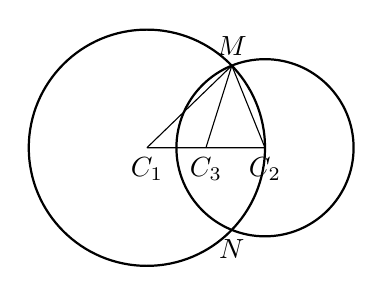
\begin{tikzpicture}[line join=round, scale=0.75]
\coordinate[label=below:{$C_1$}] (C1) at (0,0);
\coordinate[label=below:{$C_2$}] (C2) at (2,0);
\coordinate[label=below:{$C_3$}] (C3) at (1,0);
\draw[thick,name path=c1] (C1) circle (2);
\draw[thick,name path=c2] (C2) circle (1.5);
\path[name intersections={of=c1 and c2}]
    coordinate[label=above:{$M$}] (M) at (intersection-1)
    coordinate[label=below:{$N$}] (N) at (intersection-2);
\draw (C1)--(M)--(C2)--(C1) (M)--(C3);
\end{tikzpicture}
\end{figure}

\begin{align*}
&\because \left| \overrightarrow{MC_3} \right|=\left| \overrightarrow{MC_1}+\overrightarrow{MC_2} \right|/2 \\
&\therefore \left| \overrightarrow{MC_3} \right|^2=\frac{{r_1}^2+{r_2}^2+\overrightarrow{MC_1}\cdot \overrightarrow{MC_2}}{4} \\
&\because \left| \overrightarrow{C_1C_2} \right|=\left| \overrightarrow{MC_2}-\overrightarrow{MC_1} \right| \\
&\therefore \left| \overrightarrow{C_1C_2} \right|^2={r_1}^2+{r_2}^2-\overrightarrow{MC_1}\cdot \overrightarrow{MC_2} \\
&\therefore \left| \overrightarrow{MC_3} \right|^2=\frac{{r_1}^2+{r_2}^2+\left( {r_1}^2+{r_2}^2-\left| \overrightarrow{C_1C_2} \right|^2 \right)}{4}
\end{align*}






\newpage
\section{本章小结}

本章用代数的方法讨论了直线和圆。注意,我们有了第一章的知识,学习时更要注重数形结合。学习和做题时,必须从几何出发,在理解几何关系的基础上运用代数的方法。

%============================================================
\subsection{习题}

\begin{example}[拓广探索20,难度:$\star $]
已知圆$C:\left( x-1 \right) ^2+\left( y-2 \right) ^2=25$,直线$l:\left( 2m+1 \right) x+\left( m+1 \right) y-7m-4=0$。
\begin{enumerate}
    \item 求证:直线$l$恒过定点。
    \item 直线$l$被圆$C$截得的弦何时最长、何时最短?并求截得的弦长最短时$m$的值以及最短弦长。
\end{enumerate}
\end{example}

解一:

(1)恒过定点,表示取$m_1\ne m_2$生成两条直线,交点必须和$m_1,m_2$无关,联立直线方程:
\[
\begin{cases}
	\left( 2m_1+1 \right) x+\left( m_1+1 \right) y-7m_1-4=0\\
	\left( 2m_2+1 \right) x+\left( m_2+1 \right) y-7m_2-4=0\\
\end{cases}
\]
消元得$\left( m_2-m_1 \right) y-\left( m_2-m_1 \right) =0$,可见只有当$y=1$时与$m_1,m_2$无关,带入直线方程得$\left( 2m+1 \right) x-6m-3=0$,易得恒过$\left( 3,1 \right) $。

(2)易得恒定点在园内,于是弦有最短且垂直于直径方向,否则园外点可以相切,最短为0,最长弦自然是直径。略。

\begin{figure}[h]
\centering
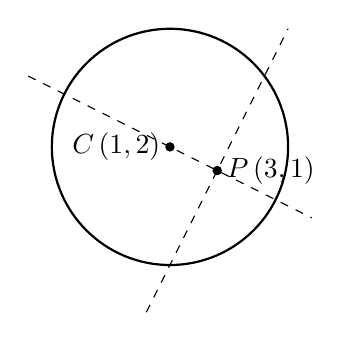
\begin{tikzpicture}[line join=round, scale=0.3]
\pgfmathparse{0.6/0.3}
\mydrawxy{0}{7}{0}{8}
\draw[thick] (1,2) circle(5);
\coordinate[label=left: {$C\left( 1,2 \right) $}] (C) at (1,2);
\coordinate[label=right:{$P\left( 3,1 \right) $}] (P) at (3,1);
\fill (C) circle (\pgfmathresult mm);
\fill (P) circle (\pgfmathresult mm);
\draw[dashed] ($(C)!-3.0!(P)$)--($(C)!3.0!(P)$) (0,-5)--(6,7);
\end{tikzpicture}
\end{figure}

解二:

(1)过恒定点的意思是有一点$\left( x_0,y_0 \right) $必然在直线上,而且不依赖于$m$的值,也就是说该点坐标的表达式中不能出现$m$,将直线写成:
\[
\left( 2x_0+y_0-7 \right) m+x_0+y_0-4=0
\]
要使之不出现$m$,则有:
\[
\begin{cases}
	2x_0+y_0-7=0\\
	x_0+y_0-4=0\\
\end{cases}
\]
可得$\left( x_0,y_0 \right) =\left( 3,1 \right) $。

\begin{tcolorbox}
理解“恒过一点”的几何含义,本题没有难度。
\end{tcolorbox}










\chapter{圆锥曲线的方程}

本章介绍3类二次曲线——椭圆、双曲线和抛物线。它们都可以通过圆锥获得,所以通称圆锥曲线,事实上,圆也是一类圆锥曲线。

本章要点:
\begin{itemize}
    \item 椭圆。
    \item 双曲线。
    \item 抛物线。
\end{itemize}

\newpage
\section{椭圆}

本节要点:
\begin{itemize}
    \item 掌握椭圆的概念;
    \item 从代数角度掌握椭圆的几何性质。
\end{itemize}

%============================================================
\subsection{椭圆及其标准方程}

\begin{definition}[椭圆]
设二维平面中有两个定点$F_1,F_2$,若平面上的点和$F_1,F_2$的距离之和都是$r>0$,则称这些点组成的集合为{\bf 椭圆},常用$E$表示,即:
\[
E:=\left\{ P \middle| \left| \overrightarrow{F_1P} \right|+\left| \overrightarrow{F_2P} \right|=r \right\}
\]
其中,$F_1,F_2$称为{\bf 焦点},$\left| \overrightarrow{F_1F_2} \right|$称为{\bf 焦距}。若令$F_1=\left( -c,0 \right) ,F_2=\left( c,0 \right) $,则椭圆可以表示为下列的{\bf 标准方程}:
\[
\frac{x^2}{a^2}+\frac{y^2}{b^2}=1
\]
其中$a,b,c$满足$a^2-b^2=c^2$。
\end{definition}

\begin{figure}[h]
\centering
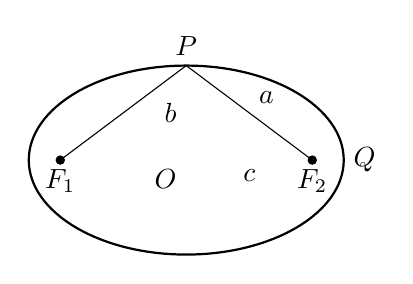
\begin{tikzpicture}[line join=round, scale=0.4]
\pgfmathparse{0.6/0.4}
\mydrawxy{-7}{7}{-5}{5}
\coordinate[label=below left:{$O$}]   (O)  at (0,0);
\coordinate[label=below:     {$F_1$}] (F1) at (-4,0);
\coordinate[label=below:     {$F_2$}] (F2) at (4,0);
\coordinate[label=above:     {$P$}]   (P)  at (0,3);
\coordinate[label=right:     {$Q$}]   (Q)  at (5,0);
\draw[thick] (0,0) ellipse (5 and 3);
\fill (F1) circle (\pgfmathresult mm);
\fill (F2) circle (\pgfmathresult mm);
\draw (F1)--(P)--(F2);
\coordinate[label=above right:{$a$}] (a) at ($(P)!0.5!(F2)$);
\coordinate[label=left:       {$b$}] (b) at ($(P)!0.5!(0,0)$);
\coordinate[label=below:      {$c$}] (c) at ($(0,0)!0.5!(F2)$);
\end{tikzpicture}
\end{figure}

\begin{tcolorbox}
详细阅读课本关于椭圆标准方程的推导过程,体会两次平方的意义。详细阅读例2、例3、例6,可以认为是椭圆的另外三种定义。
\end{tcolorbox}

%============================================================
\subsection{椭圆的简单几何性质}

设有如下椭圆,我们称:
\begin{itemize}
    \item $O,A_1,A_2,B_1,B_2$:一个{\bf 中心}和四个{\bf 顶点};
    \item $A_1A_2=2a$:{\bf 长轴};
    \item $B_1B_2=2b$:{\bf 短轴};
    \item $F_1F_2=2c$:{\bf 焦距};
    \item $e=\frac{c}{a}=\cos \theta \in \left[ 0,1 \right) $:{\bf 离心率},$e$越大椭圆越扁平,$e=0$时退化为圆,$e\rightarrow 1$时变成两条平行线$y=\pm b$。
\end{itemize}

\begin{figure}[h]
\centering
\begin{minipage}{.49\textwidth}
\centering
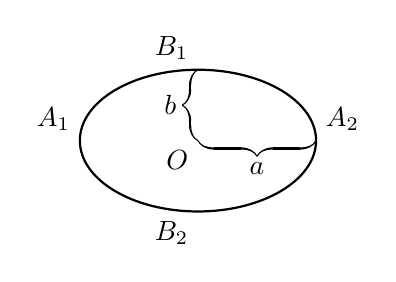
\begin{tikzpicture}[line join=round, scale=0.3]
\mydrawxy{-7}{7}{-5}{5}
\coordinate[label=below left: {$O$}]   (O)  at (0,0);
\coordinate[label=above left: {$A_1$}] (A1) at (-5,0);
\coordinate[label=above right:{$A_2$}] (A2) at (5,0);
\coordinate[label=above left: {$B_1$}] (B1) at (0,3);
\coordinate[label=below left: {$B_2$}] (B2) at (0,-3);
\draw[thick] (0,0) ellipse (5 and 3);
\coordinate[label=below:{$a$}] (a) at ($(O)!0.5!(A2)-(0,0.5)$);
\coordinate[label=left: {$b$}] (b) at ($(O)!0.5!(B1)-(0.5,0)$);
\draw[decorate,decoration={calligraphic brace,raise=0cm,aspect=0.5,amplitude=0.2cm},thick] (A2)--(O);
\draw[decorate,decoration={calligraphic brace,raise=0cm,aspect=0.5,amplitude=0.2cm},thick] (O)--(B1);
\end{tikzpicture}
\end{minipage}
\begin{minipage}{.49\textwidth}
\centering
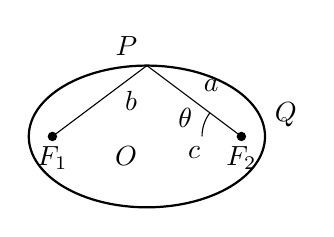
\begin{tikzpicture}[line join=round, scale=0.3]
\pgfmathparse{0.6/0.3}
\mydrawxy{-7}{7}{-5}{5}
\coordinate[label=below left:{$O$}]   (O)  at (0,0);
\coordinate[label=below:     {$F_1$}] (F1) at (-4,0);
\coordinate[label=below:     {$F_2$}] (F2) at (4,0);
\coordinate[label=above left:{$P$}]   (P)  at (0,3);
\coordinate[label=above right:{$Q$}]   (Q)  at (5,0);
\draw[thick] (0,0) ellipse (5 and 3);
\fill (F1) circle (\pgfmathresult mm);
\fill (F2) circle (\pgfmathresult mm);
\draw (F1)--(P)--(F2);
\coordinate[label=above right:{$a$}] (a) at ($(P)!0.5!(F2)$);
\coordinate[label=left:       {$b$}] (b) at ($(P)!0.5!(0,0)$);
\coordinate[label=below:      {$c$}] (c) at ($(0,0)!0.5!(F2)$);
\pic["$\theta $",draw,angle radius=0.5cm,angle eccentricity=1.5] {angle=P--F2--O};
\end{tikzpicture}
\end{minipage}
\end{figure}

%============================================================
\subsection{拓展讨论:坐标系变换}

\begin{tcolorbox}
对课本例2深入讨论。
\end{tcolorbox}

椭圆可以通过圆的拉伸获得,如下左图,圆方程为$x^2+y^2=2^2$:

\begin{figure}[h]
\centering
\begin{minipage}{.39\textwidth}
\centering
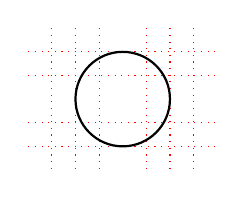
\begin{tikzpicture}[line join=round, scale=0.3]
\mydrawxy{-4}{4}{-3}{3}
\foreach \y in {-2,-1,1,2}      {\draw[dotted,red] (-4,\y)--(4,\y);}
\foreach \x in {-3,-2,-1,1,2,3} {\draw[dotted,red] (\x,3)--(\x,-3);}
\draw[thick] (0,0) circle(2);
\end{tikzpicture}
\end{minipage}
\begin{minipage}{.59\textwidth}
\centering
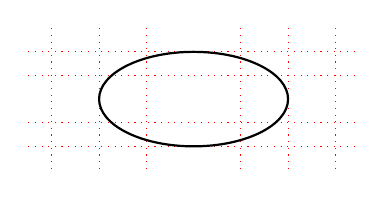
\begin{tikzpicture}[line join=round, scale=0.3]
\mydrawxy{-7}{7}{-3}{3}
\foreach \y in {-2,-1,1,2}      {\draw[dotted,red] (-7,\y)--(7,\y);}
\foreach \x in {-6,-4,-2,2,4,6} {\draw[dotted,red] (\x,3)--(\x,-3);}
\draw[thick] (0,0) ellipse (4 and 2);
\end{tikzpicture}
\end{minipage}
\end{figure}

我们进行坐标变换,将{\it x}轴拉长一倍,如上右图:
\[
\begin{cases}
	u=2x\\
	v=y\\
\end{cases}\Rightarrow \quad \begin{cases}
	x=0.5u\\
	y=v\\
\end{cases}
\]
则有:
\[
\frac{u^2}{4^2}+\frac{v^2}{2^2}=1
\]
可见,将坐标轴拉伸就可将圆变成椭圆,反之,将坐标轴压缩就可将椭圆变成圆。

%============================================================
\subsection{拓展讨论:斜率之积}

\begin{tcolorbox}
对课本例3深入讨论。
\end{tcolorbox}

设椭圆$E$及椭圆上一点$P$,如下左图,则$PA_1,PA_2$的斜率之积有:
\begin{align*}
&\because \frac{x^2}{a^2}+\frac{y^2}{b^2}=1 \\
&\therefore k_{PA_1}k_{PA_2}=\frac{y_P}{x_P+a}\cdot \frac{y_P}{x_P-a}=\frac{b^2\left( 1-\frac{{x_P}^2}{a^2} \right)}{{x_P}^2-a^2}=-\frac{b^2}{a^2}=-\tan ^2\theta
\end{align*}
特别地,当$a=b$时,$k_{PA_1}k_{PA_2}=-1$即$PA_1\bot PA_2$,此时椭圆退化为圆,如下右图。

\begin{figure}[h]
\centering
\begin{minipage}{.59\textwidth}
\centering
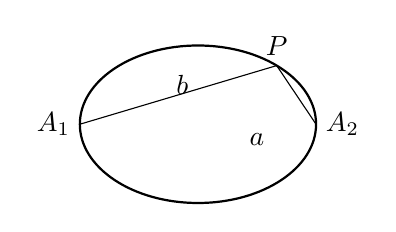
\begin{tikzpicture}[line join=round, scale=1]
\mydrawxy{-2}{2}{-1.2}{1.2}
\draw[thick] (0,0) ellipse (1.5 and 1);
\coordinate[label=left: {$A_1$}] (A1) at (-1.5,0);
\coordinate[label=right:{$A_2$}] (A2) at (1.5,0);
\coordinate[label=above:{$P$}]   (P)  at (1,0.745);
\coordinate[label=below:{$a$}] (a) at ($(0,0)!0.5!(A2)$);
\coordinate[label=left: {$b$}] (b) at ($(0,0)!0.5!(0,1)$);
\draw (A1)--(P)--(A2);
\end{tikzpicture}
\end{minipage}
\begin{minipage}{.39\textwidth}
\centering
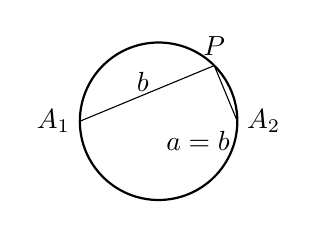
\begin{tikzpicture}[line join=round, scale=1]
\mydrawxy{-2}{2}{-1.2}{1.2}
\draw[thick] (0,0) circle(1);
\coordinate[label=left: {$A_1$}] (A1) at (-1,0);
\coordinate[label=right:{$A_2$}] (A2) at (1,0);
\coordinate[label=above:{$P$}]   (P)  at (0.707,0.707);
\coordinate[label=below:{$a=b$}] (a) at ($(0,0)!0.5!(A2)$);
\coordinate[label=left: {$b$}]   (b) at ($(0,0)!0.5!(0,1)$);
\draw (A1)--(P)--(A2);
\end{tikzpicture}
\end{minipage}
\end{figure}

可见:
\begin{itemize}
    \item $k_1k_2\in \left( -\infty ,-1 \right) $:长条形椭圆;
    \item $k_1k_2=-1$:圆;
    \item $k_1k_2\in \left( -1,0 \right) $:扁宽形椭圆。
\end{itemize}

%============================================================
\subsection{拓展讨论:两个焦点}

\begin{tcolorbox}
对课本例5深入讨论。
\end{tcolorbox}

例5说明了从任意一个焦点出发的光线都能聚焦到另一个焦点,证明这点需要微积分的知识,略。但我们可以思考,当两个焦点重合的时候,从焦点出发的任意光线都能返回到焦点,这是一个圆,而且圆的半径总是垂直于切线。

\begin{figure}[h]
\centering
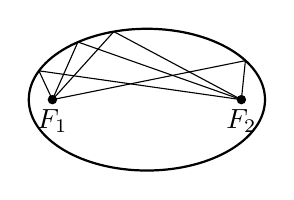
\begin{tikzpicture}[line join=round, scale=0.3]
\pgfmathparse{0.6/0.3}
\mydrawxy{-6}{6}{-3.5}{3.5}
\draw[thick] (0,0) ellipse (5 and 3);
\coordinate[label=below:{$F_1$}] (F1) at (-4,0);
\coordinate[label=below:{$F_2$}] (F2) at (4,0);
\fill (F1) circle (\pgfmathresult mm);
\fill (F2) circle (\pgfmathresult mm);
\coordinate (A) at (-4.57,1.22);
\coordinate (B) at (-2.92,2.44);
\coordinate (C) at (-1.4,2.88);
\coordinate (D) at (4.17,1.65);
\foreach \p in {A,B,C,D} {\draw (F1)--(\p)--(F2);}
\end{tikzpicture}
\end{figure}

有些音乐厅就设计成椭圆,乐队位于一个焦点附近,VIP位于另一个焦点附近,使得VIP在听觉上能位于乐队中。

%============================================================
\subsection{拓展讨论:动点距离直线}

\begin{tcolorbox}
对课本例6深入讨论。
\end{tcolorbox}

我们考察,对于任意一个椭圆$E$,是否必有垂直坐标轴的直线$x=x_0$,且椭圆上的点$P$距离焦点和直线的比是定值$k$。

\begin{figure}[h]
\centering
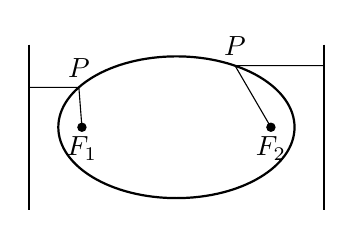
\begin{tikzpicture}[line join=round, scale=0.3]
\pgfmathparse{0.6/0.3}
\mydrawxy{-7}{7}{-3.5}{3.5}
\draw[thick] (0,0) ellipse (5 and 3);
\coordinate[label=below:{$F_1$}] (F1) at (-4,0);
\coordinate[label=below:{$F_2$}] (F2) at (4,0);
\coordinate[label=above:{$P$}]   (P1) at (-4.13,1.69);
\coordinate[label=above:{$P$}]   (P2) at (2.48,2.61);
\fill (F1) circle (\pgfmathresult mm);
\fill (F2) circle (\pgfmathresult mm);
\draw[thick] (-6.25,3.5)--(-6.25,-3.5) (6.25,3.5)--(6.25,-3.5);
\draw (F1)--(P1)--(-6.25,1.69) (F2)--(P2)--(6.25,2.61);
\end{tikzpicture}
\end{figure}

距离焦点和直线的比:
\begin{align*}
&\frac{x^2}{a^2}+\frac{y^2}{b^2}=1 \\
&k=\frac{\sqrt{\left( x\pm c \right) ^2+y^2}}{\left| x-x_0 \right|}\Rightarrow k^2\left( x-x_0 \right) ^2=\left( x\pm c \right) ^2+y^2
\end{align*}
化简后得:
\[
\left( 1-k^2-\frac{b^2}{a^2} \right) x^2+2\left( k^2x_0\pm c \right) x+\left( a^2-k^2{x_0}^2 \right) =0
\]
若要对所有$x$都成立,必须:
\[
\begin{cases}
	1-k^2-\frac{b^2}{a^2}=0\\
	k^2x_0\pm c=0\\
	a^2-k^2{x_0}^2=0\\
\end{cases}\Rightarrow \quad \begin{cases}
	k=\frac{c}{a}\in \left( 0,1 \right) \\
	x_0=\mp \frac{a^2}{c}\\
\end{cases}
\]
不难发现特点:
\begin{itemize}
    \item 对于左焦点有左边的直线$x=-\frac{a^2}{c}$,对于右焦点有右边的直线$x=\frac{a^2}{c}$,且两条直线一定在椭圆外侧;
    \item 动点距离焦点更近;
    \item 当$c=0$时椭圆退化为圆,且$x_0=\pm \infty ,k=0$,表示直线为无穷远处,自行脑补。
\end{itemize}

%============================================================
\subsection{拓展讨论:椭圆的一般方程}

教材中对于直线和圆都有一般形式的方程,为什么椭圆就没有?我们来推导一下椭圆方程的一般形式,从最一般的二次曲线开始,如下:
\[
Ax^2+By^2+Cxy+Dx+Ey+F=0
\]
$A,D$和$B,E$可以凑出$x,y$的平方项,一方面只影响$F$,另一方面$x,y$的平方项可以通过坐标平移解决,所以我们可以之分析如下形式:
\[
Ax^2+By^2+Cxy+F=0
\]
易得该方程对应的曲线关于原点对称。

我们先考察另一个问题,将椭圆绕中心点沿顺时针转$\alpha $后方程是什么样子的。设椭圆如下:
\[
\frac{x^2}{a^2}+\frac{y^2}{b^2}=1
\]
转换为极坐标形式:
\[
\frac{\left( r\cos \theta \right) ^2}{a^2}+\frac{\left( r\sin \theta \right) ^2}{b^2}=1
\]
将椭圆绕中心点沿顺时针转$\alpha $:
\[
\frac{\left[ r\cos \left( \theta -\alpha \right) \right] ^2}{a^2}+\frac{\left[ r\sin \left( \theta -\alpha \right) \right] ^2}{b^2}=1 \qquad \alpha \in \left[ 0,\pi \right)
\]
注意我们这里是顺时针转动图形,相当于逆时针转动坐标系,所以是$-\alpha $而不是$+\alpha $,展开后:
\begin{align*}
&\left( b^2\cos ^2\alpha +a^2\sin ^2\alpha \right) x^2+\left( b^2\sin ^2\alpha +a^2\cos ^2\alpha \right) y^2-c^2\sin 2\alpha xy=a^2b^2 \\
&Ax^2+By^2+Cxy+F=0 \\
&\begin{cases}
	A=b^2\cos ^2\alpha +a^2\sin ^2\alpha =b^2+\frac{c^2}{2}\left( 1-\cos 2\alpha \right)\\
	B=b^2\sin ^2\alpha +a^2\cos ^2\alpha =b^2+\frac{c^2}{2}\left( 1+\cos 2\alpha \right)\\
	C=-c^2\sin 2\alpha\\
	F=-a^2b^2\\
\end{cases}
\end{align*}
不难发现:
\begin{itemize}
    \item $F<0$,若$F>0$则曲线不存在,若$F=0$则有可能是一点有可能是直线;
    \item $A,B>0$,否则变成双曲线,且有$A+B=a^2+b^2$,当$A=B$时$\alpha =\pi /4$或$3\pi /4$;
    \item $A,F>0$共同决定了椭圆和{\it x}轴的交点,$B,F>0$共同决定了椭圆和{\it y}轴的交点。
\end{itemize}
特别地,当$\alpha =\pi /4$时,方程为在圆的基础上加一个$xy$项,如下:
\[
\left( a^2+b^2 \right) x^2+\left( a^2+b^2 \right) y^2-2c^2xy=2a^2b^2
\]
当$\alpha =\pi /2$时,表现为长短轴互换,如下:
\[
a^2x^2+b^2y^2=a^2b^2
\]

%============================================================
\subsection{习题}

\begin{example}[复习巩固6,难度:$\star $]
如图,圆$O$的半径为定长$r$,$A$是圆$O$内一个定点,$P$是圆$O$上任意一点。线段$AP$的垂直平分线$l$和半径$OP$相交于点$Q$,当点$P$在圆上运动时,点$Q$的轨迹是什么?为什么?
\end{example}

\begin{figure}[h]
\centering
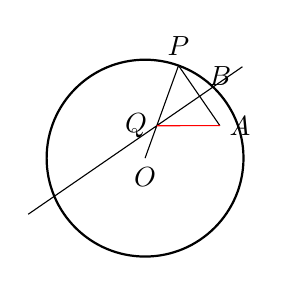
\begin{tikzpicture}[line join=round, scale=1.25]
\draw[thick] (0,0) circle(1);
\coordinate[label=below:      {$O$}] (O) at (0,0);
\coordinate[label=above:      {$P$}] (P) at (0.34,0.94);
\coordinate[label=right:      {$A$}] (A) at (0.76,0.33);
\coordinate[label=above right:{$B$}] (B) at ($(P)!0.5!(A)$);
\coordinate[label=left:       {$Q$}] (Q) at ($(O)!0.35!(P)$);
\draw (O)--(P)--(A) ($(Q)!-3.0!($(P)!(Q)!(A)$)$)--($(Q)!2.0!($(P)!(Q)!(A)$)$);
\draw[red] (Q)--(A);
\end{tikzpicture}
\end{figure}

解:

连接$QA$,有:
\[
QO+QA=QO+QP=r
\]

\begin{tcolorbox}
仔细观察图形,本题没有难度。不要盲目建立坐标系,椭圆的中心未知。
\end{tcolorbox}

~

\begin{example}[拓广探索14,难度:$\star $]
已知椭圆$\frac{x^2}{4}+\frac{y^2}{9}=1$,一组平行直线的斜率是$\frac{3}{2}$。
\begin{enumerate}
    \item 这组直线何时与椭圆有两个公共点?
    \item 当它们与椭圆有两个公共点时,证明这些直线被椭圆截得的线段的中点在同一条直线上。
\end{enumerate}
\end{example}

解:

(1)略。

(2)一般的做法是假设直线$y=\frac{3}{2}x+c$,带入椭圆求交点:
\begin{align*}
&18x^2+12cx+4c^2-36=0 \\
&x_{1,2}=\frac{-12c\pm \sqrt{144c^2-4\cdot 18\cdot \left( 4c^2-36 \right)}}{36}
\end{align*}
得到线段中点:
\[
\begin{cases}
	x_0=-\frac{1}{3}c\\
	y_0=\frac{1}{2}\\
\end{cases}
\]
是一个参数方程,就是一条过原点,斜率是$-3/2$的直线。

但是,理解了坐标系变换,可以先压缩{\it xy}两个轴,使得椭圆变成一个标注圆,此时,这一组平行线将变成:
\[
y=x+c
\]
不难发现割线的中点是直线$y=-x$,最后通过拉伸{\it xy}两个轴变回来,略。

\begin{tcolorbox}
本题没有难度,但从坐标系变换的角度分析,还是有点意思的。
\end{tcolorbox}






\newpage
\section{双曲线}

本节要点:
\begin{itemize}
    \item 掌握双曲线的概念;
    \item 从代数角度掌握双曲线的几何性质。
\end{itemize}

%============================================================
\subsection{双曲线及其标准方程}

\begin{definition}[双曲线]
设二维平面中有两个定点$F_1,F_2$,若平面上的点和$F_1,F_2$的距离之差的绝对值都是$r>0$,则称这些点组成的集合为{\bf 双曲线},常用$H$表示,即:
\[
H:=\left\{ P \middle| \left| \left| \overrightarrow{F_1P} \right|-\left| \overrightarrow{F_2P} \right| \right|=r \right\}
\]
其中,$F_1,F_2$称为{\bf 焦点},$\left| \overrightarrow{F_1F_2} \right|$称为{\bf 焦距}。若令$F_1=\left( -c,0 \right) ,F_2=\left( c,0 \right) $,则双曲线可以表示为下列的{\bf 标准方程}:
\[
\frac{x^2}{a^2}-\frac{y^2}{b^2}=1
\]
其中$a,b,c$满足$a^2+b^2=c^2$。
\end{definition}

\begin{figure}[h]
\centering
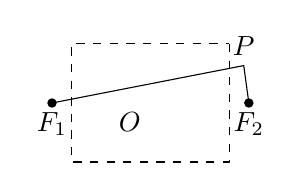
\begin{tikzpicture}[line join=round, scale=0.25]
\pgfmathparse{0.6/0.25}
\mydrawxy{-7}{7}{-5}{5}
\mydrawhyperbola{7}{4}{3}
\coordinate[label=below left:{$O$}]   (O)  at (0,0);
\coordinate[label=below:     {$F_1$}] (F1) at (-5,0);
\coordinate[label=below:     {$F_2$}] (F2) at (5,0);
\coordinate[label=above:     {$P$}]   (P)  at (4.74,1.90);
\fill (F1) circle (\pgfmathresult mm);
\fill (F2) circle (\pgfmathresult mm);
\draw (F1)--(P)--(F2);
\draw[dashed] (4,3)--(4,-3)--(-4,-3)--(-4,3)--(4,3);
\end{tikzpicture}
\end{figure}

\begin{tcolorbox}
详细阅读课本关于双曲线标准方程的推导过程,体会两次平方的意义。详细阅读例6,可以认为是双曲线的另外的定义。
\end{tcolorbox}

%============================================================
\subsection{双曲线的简单几何性质}

双曲线图形如下,我们称:
\begin{itemize}
    \item $O,A_1,A_2,B_1,B_2$:一个{\bf 中心}和四个{\bf 顶点};
    \item $A_1A_2=2a$:{\bf 实轴};
    \item $B_1B_2=2b$:{\bf 虚轴};
    \item $F_1F_2=2c$:{\bf 焦距};
    \item $e=\frac{c}{a}=\frac{1}{\cos \theta}\in \left( 1,+\infty \right) $:{\bf 离心率},$e$越大双曲线开口越大;
    \item $y=\pm \frac{b}{a}x$:{\bf 渐近线}。
\end{itemize}

\begin{figure}[h]
\centering
\begin{tikzpicture}[line join=round, scale=0.5]
\pgfmathparse{0.6/0.5}
\mydrawxy{-7}{7}{-5}{5}
\mydrawhyperbola{7}{4}{3}
\coordinate[label=below left: {$O$}]   (O)  at (0,0);
\coordinate[label=below:      {$F_1$}] (F1) at (-5,0);
\coordinate[label=below:      {$F_2$}] (F2) at (5,0);
\coordinate[label=below right:{$A_1$}] (A1) at (-4,0);
\coordinate[label=below left: {$A_2$}] (A2) at (4,0);
\coordinate[label=above left: {$B_1$}] (B1) at (0,3);
\coordinate[label=below left: {$B_2$}] (B2) at (0,-3);
\fill (F1) circle (\pgfmathresult mm);
\fill (F2) circle (\pgfmathresult mm);
\draw[dashed] ($(A2)+(B1)$)--($(A2)+(B2)$)--($(A1)+(B2)$)--($(A1)+(B1)$)--($(A2)+(B1)$);
\draw[dashed] ($(O)!1.7!($(A1)+(B2)$)$)--($(O)!1.7!($(A2)+(B1)$)$) ($(O)!1.7!($(A1)+(B1)$)$)--($(O)!1.7!($(A2)+(B2)$)$);
\coordinate[label=above:{$a$}] (a) at ($(0,3)!0.5!(4,3)+(0,0.5)$);
\draw[decorate,decoration={calligraphic brace,raise=0cm,aspect=0.5,amplitude=0.2cm},thick] (0,3)--(4,3);
\coordinate[label=right:{$b$}] (b) at ($(4,3)!0.5!(4,0)+(0.5,0)$);
\draw[decorate,decoration={calligraphic brace,raise=0cm,aspect=0.5,amplitude=0.2cm},thick] (4,3)--(4,0);
\coordinate (t) at (4,3);
\pic["$\theta $",draw,angle radius=0.5cm,angle eccentricity=1.5] {angle=F2--O--t};
\end{tikzpicture}
\end{figure}

%============================================================
\subsection{拓展讨论:坐标系变换}

同椭圆,略。

%============================================================
\subsection{拓展讨论:斜率之积}

设双曲线$H$及双曲线上一点$P$,则$PA_1,PA_2$的斜率之积有:
\begin{align*}
&\because \frac{x^2}{a^2}-\frac{y^2}{b^2}=1 \\
&\therefore k_{PA_1}k_{PA_2}=\frac{y_P}{x_P+a}\cdot \frac{y_P}{x_P-a}=\frac{b^2\left( \frac{{x_P}^2}{a^2}-1 \right)}{{x_P}^2-a^2}=\frac{b^2}{a^2}=\tan ^2\theta
\end{align*}

\begin{figure}[h]
\centering
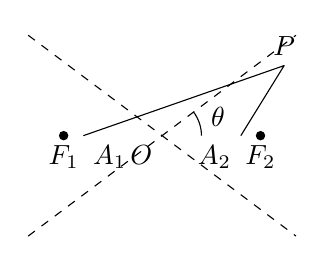
\begin{tikzpicture}[line join=round, scale=0.25]
\pgfmathparse{0.6/0.25}
\mydrawxy{-7}{7}{-5}{5}
\mydrawhyperbola{7}{4}{3}
\coordinate[label=below left: {$O$}]   (O)  at (0,0);
\coordinate[label=below:      {$F_1$}] (F1) at (-5,0);
\coordinate[label=below:      {$F_2$}] (F2) at (5,0);
\coordinate[label=below right:{$A_1$}] (A1) at (-4,0);
\coordinate[label=below left: {$A_2$}] (A2) at (4,0);
\coordinate[label=above:      {$P$}]   (P)  at (6.20,3.56);
\fill (F1) circle (\pgfmathresult mm);
\fill (F2) circle (\pgfmathresult mm);
\draw (A1)--(P)--(A2);
\draw[dashed] ($(O)!1.7!(-4,-3)$)--($(O)!1.7!(4,3)$) ($(O)!1.7!(-4,3)$)--($(O)!1.7!(4,-3)$);
\coordinate (t) at (4,3);
\pic["$\theta $",draw,angle radius=0.5cm,angle eccentricity=1.5] {angle=F2--O--t};
\end{tikzpicture}
\end{figure}

%============================================================
\subsection{拓展讨论:两个焦点}

从任意一个焦点出发的光线都可以视作从另一个焦点发出,证明这点需要微积分的知识,略。

\begin{figure}[ht]
\centering
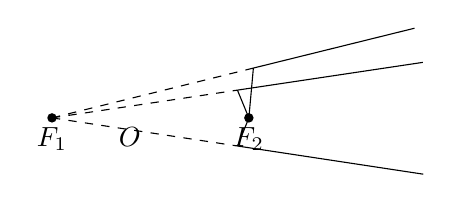
\begin{tikzpicture}[line join=round, scale=0.25]
\pgfmathparse{0.6/0.25}
\mydrawxy{-7}{7}{-5}{5}
\mydrawhyperbola{7}{4}{3}
\coordinate[label=below left:{$O$}]   (O)  at (0,0);
\coordinate[label=below:     {$F_1$}] (F1) at (-5,0);
\coordinate[label=below:     {$F_2$}] (F2) at (5,0);
\coordinate                           (P1) at (5.23,2.53);
\coordinate                           (P2) at (4.42,1.41);
\coordinate                           (P3) at (4.43,-1.43);
\fill (F1) circle (\pgfmathresult mm);
\fill (F2) circle (\pgfmathresult mm);
\draw (F2)--(P1) (F2)--(P2) (F2)--(P3);
\draw[dashed] (F1)--(P1) (F1)--(P2) (F1)--(P3);
\draw (P1)--($(P1)!-0.8!(F1)$) (P2)--($(P2)!-1.0!(F1)$) (P3)--($(P3)!-1.0!(F1)$);
\end{tikzpicture}
\end{figure}

%============================================================
\subsection{拓展讨论:动点距离直线}

\begin{tcolorbox}
对课本例5深入讨论。
\end{tcolorbox}

我们考察,对于任意一个椭圆$E$,是否必有垂直坐标轴的直线$x=x_0$,且椭圆上的点$P$距离焦点和直线的比是定值$k$。

\begin{figure}[h]
\centering
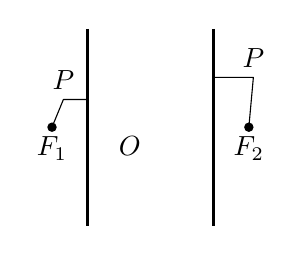
\begin{tikzpicture}[line join=round, scale=0.25]
\pgfmathparse{0.6/0.25}
\mydrawxy{-7}{7}{-5}{5}
\mydrawhyperbola{7}{4}{3}
\coordinate[label=below left:{$O$}]   (O)  at (0,0);
\coordinate[label=below:     {$F_1$}] (F1) at (-5,0);
\coordinate[label=below:     {$F_2$}] (F2) at (5,0);
\coordinate[label=above:     {$P$}]   (P1) at (-4.42,1.41);
\coordinate[label=above:     {$P$}]   (P2) at (5.23,2.53);
\fill (F1) circle (\pgfmathresult mm);
\fill (F2) circle (\pgfmathresult mm);
\draw[thick] (-3.2,5)--(-3.2,-5) (3.2,5)--(3.2,-5);
\draw (-3.2,1.41)--(P1)--(F1);
\draw (3.2,2.53)--(P2)--(F2);
\end{tikzpicture}
\end{figure}

距离焦点和直线的比:
\begin{align*}
&\frac{x^2}{a^2}-\frac{y^2}{b^2}=1 \\
&k=\frac{\sqrt{\left( x\pm c \right) ^2+y^2}}{\left| x-x_0 \right|}\Rightarrow k^2\left( x-x_0 \right) ^2=\left( x\pm c \right) ^2+y^2
\end{align*}
化简后得:
\[
\left( 1-k^2+\frac{b^2}{a^2} \right) x^2+2\left( k^2x_0\pm c \right) x+\left( a^2-k^2{x_0}^2 \right) =0
\]
若要对所有$x$都成立,必须:
\[
\begin{cases}
	1-k^2+\frac{b^2}{a^2}=0\\
	k^2x_0\pm c=0\\
	a^2-k^2{x_0}^2=0\\
\end{cases}\Rightarrow \quad \begin{cases}
	k=\frac{c}{a}\in \left( 1,+\infty \right) \\
	x_0=\mp \frac{a^2}{c}\\
\end{cases}
\]
不难发现特点:
\begin{itemize}
    \item 对于左焦点有左边的直线$x=-\frac{a^2}{c}$,对于右焦点有右边的直线$x=\frac{a^2}{c}$,且两条直线一定在双曲线内侧;
    \item 动点距离直线更近。
\end{itemize}

%============================================================
\subsection{拓展讨论:双曲线的一般方程}

我们来推导一下双曲线方程的一般形式。中心点平移的讨论见椭圆,我们直接从旋转开始。双曲线的采用极坐标的形式,双曲线绕中心点沿顺时针转$\alpha $后的方程如下:
\[
\frac{\left[ r\cos \left( \theta -\alpha \right) \right] ^2}{a^2}-\frac{\left[ r\sin \left( \theta -\alpha \right) \right] ^2}{b^2}=1 \qquad \alpha \in \left[ 0,\pi \right)
\]
注意我们这里是顺时针转动图形,相当于逆时针转动坐标系,所以是$-\alpha $而不是$+\alpha $,展开后:
\begin{align*}
&\left( b^2\cos ^2\alpha -a^2\sin ^2\alpha \right) x^2+\left( b^2\sin ^2\alpha -a^2\cos ^2\alpha \right) y^2+c^2\sin 2\alpha xy=a^2b^2 \\
&Ax^2+By^2+Cxy+F=0 \\
&\begin{cases}
	A=b^2\cos ^2\alpha -a^2\sin ^2\alpha =\frac{c^2}{2}\left( 1+\cos 2\alpha \right) -a^2\\
	B=b^2\sin ^2\alpha -a^2\cos ^2\alpha =\frac{c^2}{2}\left( 1-\cos 2\alpha \right) -a^2\\
	C=c^2\sin 2\alpha\\
	F=-a^2b^2\\
\end{cases}
\end{align*}
不难发现:
\begin{itemize}
    \item $F<0$,若$F>0$则曲线不存在,若$F=0$则有可能是一点有可能是直线,这点同椭圆;
    \item $A+B=b^2-a^2,A-B=c^2\cos 2\alpha $,当$A=B$时$\alpha =\pi /4$或$3\pi /4$。
\end{itemize}
特别地,当$\alpha =\pi /4$时,方程为在圆的基础上加一个$xy$项,如下:
\[
\frac{b^2-a^2}{2}x^2+\frac{b^2-a^2}{2}y^2+c^2xy=a^2b^2
\]
当$\alpha =\pi /2$时,表现为实轴虚轴互换,如下:
\[
-a^2x^2+b^2y^2=a^2b^2
\]

%============================================================
\subsection{拓展讨论:\texorpdfstring{$y=\frac{1}{x}$}{y=1/x}和\texorpdfstring{$y=x+\frac{1}{x}$}{y=x+1/x}}

继续上面的讨论,若有$a=b=\sqrt{2}$,则双曲线为:
\[
\frac{x^2}{2}-\frac{y^2}{2}=1
\]
显然$y=\pm x$是它的两条渐近线。当我们沿顺时针旋转$\pi /4$后:
\begin{align*}
&\frac{b^2-a^2}{2}x^2+\frac{b^2-a^2}{2}y^2+c^2xy=a^2b^2 \\
&\because a=b=\sqrt{2},c=2 \\
&\therefore xy=1
\end{align*}
这也是为什么之前碰到的$y=\frac{1}{x}$也称为双曲线的原因。

\begin{figure}[h]
\centering
\begin{tikzpicture}[line join=round, scale=0.25]
\pgfmathparse{0.6/0.25}
\mydrawxy{-7}{7}{-5}{5}
\mydrawhyperbola{5}{1.414}{1.414}
\draw[thick,domain=0.2:5,samples=200]   plot (\x,{1/\x});
\draw[thick,domain=-5:-0.2,samples=200] plot (\x,{1/\x});
\end{tikzpicture}
\end{figure}

对于$y=x+\frac{1}{x}$,两边同乘以$x$可得:
\[
x^2-xy+1=0
\]
其实就是压缩了开口,再沿顺时针转$3\pi /8$,具体分析略,可借助GeoGebra研究其变化。

%============================================================
\subsection{习题}

\begin{example}[综合运用11,难度:$\star $]
$M$是一个动点,$MA$与直线$y=x$垂直,垂足$A$位于第一象限,$MB$与直线$y=-x$垂直,垂足$B$位于第四象限。若四边形$OAMB$($O$为原点)的面积为3,求动点$M$的轨迹方程。
\end{example}

解:

本题一步步解不难,略。实际为图象$xy=3$绕原点按顺时针转$\pi /4$,自然是双曲线。

我们要考察的是若这两条线为任意的$y_1=k_1x,y_2=k_2x$,以动点和原点加上这两条直线组成的平行四边形$OAMB$的面积为定值$S$,动点$M$的轨迹方程是否为双曲线。根据上面的讨论,其实是双曲线,$y_1=k_1x,y_2=k_2x$是两条渐近线。

\begin{tcolorbox}
本题本身没有难度,但之后我们的思考很有意思。
\end{tcolorbox}

~

\begin{example}[拓广探索13,难度:$\star $]
已知双曲线$x^2-\frac{y^2}{2}=1$,过点$P\left( 1,1 \right) $的直线$l$与双曲线相交于$A,B$两点,$P$能否是线段$AB$的中点?为什么?
\end{example}

解:

易得$P$在双曲线中间,于是可设直线:
\[
y-1=k\left( x-1 \right)
\]
带入双曲线方程,求得交点坐标:
\[
x=\frac{k\left( 1-k \right) \pm \sqrt{k^2\left( 1-k \right) ^2+\left( 2-k^2 \right) \cdot \left[ \left( 1-k \right) ^2+2 \right]}}{\left( 2-k^2 \right)}
\]
若有焦点,则通过中心点求得$k$:
\[
x=\frac{k\left( 1-k \right)}{2-k^2}=1\Rightarrow k=2
\]
验证此时:
\[
\varDelta =4+\left( -2 \right) \cdot 3<0
\]
实际无交点,所以没有这样的直线。

\begin{tcolorbox}
本题没有难度。
\end{tcolorbox}

~

\begin{example}[拓广探索14,难度:$\star \star $]
一直双曲线$\frac{x^2}{4}-\frac{y^2}{16}=1$与直线$l:y=kx+m,k\ne \pm 2$有唯一的公共点$M$,过点$M$且与$l$垂直的直线分别交{\it x}轴、{\it y}轴于$A\left( x,0 \right) ,B\left( 0,y \right) $两点。当点$M$运动时,求点$P\left( x,y \right) $的轨迹方程,并说明轨迹是什么曲线。如果推广到一般双曲线,能得到什么相应的结论?
\end{example}

解:

将直线带入双曲线得到:
\[
\left( 4-k^2 \right) x^2-2kmx-\left( m^2+16 \right) =0
\]
根据题意要求:
\begin{align*}
&\varDelta =16\left( m^2-4k^2+16 \right) =0\Rightarrow m^2=4\left( k^2-4 \right) \\
&x_{1,2}=\frac{km\pm 2\sqrt{m^2-4k^2+16}}{4-k^2}
\end{align*}
得到$M$坐标:
\[
M=\left( x_M,y_M \right) =\left( -\frac{4k}{m},-\frac{16}{m} \right)
\]
于是过$M$垂直于$l$的直线:
\[
y+\frac{16}{m}=-\frac{1}{k}\left( x+\frac{4k}{m} \right)
\]
$P$坐标:
\[
P=\left( x_{y=0},y_{x=0} \right) =\left( -\frac{20k}{m},-\frac{20}{m} \right)
\]
是一个参数方程,结合$\varDelta =0$可化简为:
\[
\frac{x^2}{100}-\frac{y^2}{25}=1
\]
题中的一个交点显然$l$是双曲线的切线,又由于$l$是通过斜距式给出,所以$k\in \left( -\infty ,-2 \right) \cup \left( 2,+\infty \right) $,所以$P$的轨迹是双曲线但是不包括顶点。

对于一般的双曲线方程,有:
\begin{align*}
&H:\frac{x^2}{a^2}-\frac{y^2}{b^2}=1 \\
&H\cap l:\left( b^2-a^2k^2 \right) x^2-2a^2kmx-\left( a^2m^2+a^2b^2 \right) =0 \\
&x_{1,2}=\frac{a^2km\pm ab\sqrt{b^2+m^2-a^2k^2}}{b^2-a^2k^2}\text{且}-m^2=b^2-a^2k^2 \\
&M=\left( x_M,y_M \right) =\left( -\frac{a^2k}{m},-\frac{b^2}{m} \right) \\
&l_{\bot}:y+\frac{b^2}{m}=-\frac{1}{k}\left( x+\frac{a^2k}{m} \right) \\
&P=\left( -\frac{\left( a^2+b^2 \right) k}{m},-\frac{a^2+b^2}{m} \right)
\end{align*}

\begin{tcolorbox}
本题思路明显,但是计算量大。
\end{tcolorbox}






\newpage
\section{抛物线}

本节要点:
\begin{itemize}
    \item 掌握抛物线的概念;
    \item 从代数角度掌握抛物线的几何性质。
\end{itemize}

%============================================================
\subsection{抛物线及其标准方程}

\begin{definition}[抛物线]
设二维平面中有两个定点$F$和直线$l$,设它们距离为$p>0$,若平面上的点和$F,l$的距离相等,则称这些点组成的集合为{\bf 抛物线},常用$P$表示,若令$F=\left( \frac{p}{2},0 \right) ,l:x=-\frac{p}{2}$,则抛物线可以表示为下列的{\bf 标准方程}:
\[
y=2px \quad p>0
\]
其中,$F$称为{\bf 焦点},$l$称为{\bf 准线}。
\end{definition}

\begin{figure}[h]
\centering
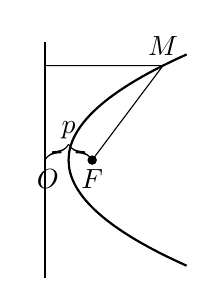
\begin{tikzpicture}[line join=round, scale=0.3]
\pgfmathparse{0.6/0.3}
\mydrawxy{-7}{7}{-5}{5}
\draw[thick,domain=0:5,samples=200] plot (\x,{ sqrt(4*(\x))}); % p=2
\draw[thick,domain=0:5,samples=200] plot (\x,{-sqrt(4*(\x))});
\coordinate[label=below left:{$O$}] (O) at (0,0);
\coordinate[label=below:     {$F$}] (F) at (1,0);
\coordinate[                      ] (K) at (-1,0);
\coordinate[label=above:     {$M$}] (M) at (4,4);
\draw[thick] (-1,5)--(-1,-5);
\draw (-1,4)--(M)--(F);
\fill (F) circle (\pgfmathresult mm);
\coordinate[label=above:{$p$}] (p) at ($(O)+(0,0.5)$);
\draw[decorate,decoration={calligraphic brace,raise=0cm,aspect=0.5,amplitude=0.2cm},thick] (K)--(F);
\end{tikzpicture}
\end{figure}

\begin{tcolorbox}
详细阅读课本关于双曲线标准方程的推导过程,体会两次平方的意义。详细阅读例2、例4、例5。
\end{tcolorbox}

%============================================================
\subsection{抛物线的简单几何性质}

我们称:
\begin{itemize}
    \item $y=0$:{\bf 轴};
    \item $\left( 0,0 \right) $:{\bf 顶点};
    \item $e=1$:{\bf 离心率},恒为1。
\end{itemize}

%============================================================
\subsection{拓展讨论:焦点}

从焦点出发的光线经抛物线反射成平行光,沿抛物线的轴入射的平行光汇聚于焦点,证明这点需要微积分的知识,略。

\begin{figure}[ht]
\centering
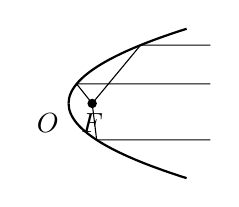
\begin{tikzpicture}[line join=round, scale=0.3]
\pgfmathparse{0.6/0.3}
\mydrawxy{-7}{7}{-4}{4}
\draw[thick,domain=0:5,samples=200] plot (\x,{ sqrt(2*(\x))});
\draw[thick,domain=0:5,samples=200] plot (\x,{-sqrt(2*(\x))});
\coordinate[label=below left:{$O$}] (O)  at (0,0);
\coordinate[label=below:     {$F$}] (F)  at (1,0);
\coordinate                         (P1) at (3.05,2.47);
\coordinate                         (P2) at (0.34,0.83);
\coordinate                         (P3) at (1.19,-1.54);
\fill (F) circle (\pgfmathresult mm);
\draw (F)--(P1)--(6,2.47);
\draw (F)--(P2)--(6,0.83);
\draw (F)--(P3)--(6,-1.54);
\end{tikzpicture}
\end{figure}

反射式望远镜就是由抛物面和双曲线构成,抛物面的焦点和双曲面的一个焦点重合。遥远的星体发出的光线可以认为是平行光,到达抛物面反射后汇聚于焦点,再由双曲面反射,形成的虚像位于双曲面的另一个焦点,这样,星体就像位于双曲面的另一个焦点一样,使得星体看起来更近了,详见教材本章小结的拓广探索15。

对于焦点,我们还可以这么思考。设有$F_1,F_2$两个焦点,若从$F_1$射出的光线经曲线反射汇聚于$F_2$,则曲线构成椭圆。当$F_2$逐渐远离$F_1$,椭圆变得越来越扁平,当$F_2$置于无穷远处时,光线经曲线反射称为平行线,此时椭圆变成了抛物线。对于离心率:
\[
\lim_{c\rightarrow a} e=\lim_{c\rightarrow a} \frac{c}{a}=1
\]

%============================================================
\subsection{拓展讨论:抛物线的一般方程}

采用极坐标的形式,抛物线绕顶点沿顺时针转$\alpha $后的方程如下:
\begin{align*}
&y^2=2px \\
&\left[ r\sin \left( \theta -\alpha \right) \right] ^2=2pr\cos \left( \theta -\alpha \right) \\
&\cos ^2\alpha \cdot y^2-\sin 2\alpha \cdot xy+\sin ^2\alpha \cdot x^2=2p\cos \alpha \cdot x+2p\sin \alpha \cdot y
\end{align*}
注意我们这里是顺时针转动图形,相当于逆时针转动坐标系,所以是$-\alpha $而不是$+\alpha $。对比椭圆和双曲线,不难发现,抛物线的特征是有关于$x,y$的一次项。






\newpage
\section{本章小结}

本章讨论了三类圆锥曲线,椭圆、双曲线和抛物线,它们都是由一个平面切圆锥构成,所以统称为圆锥曲线。学习时要多画图,多从几何理解曲线的方程。










\chapter{数列}

本章介绍数列。

本章要点:
\begin{itemize}
    \item 等差数列。
    \item 等比数列。
\end{itemize}

\begin{tcolorbox}
数列可以看出是函数的离散化,所以学习过程中特别要注意和函数的联系。
\end{tcolorbox}

\newpage
\section{数列的概念}

本节要点:
\begin{itemize}
    \item 掌握数列的概念;
    \item 掌握数列前$n$项和的概念。
\end{itemize}

~

数列及其前$n$项的和没有难度。反复体会本节第2个思考题,如何从$S_n$推导$a_n$,具有典型意义。

注意两点:
\begin{itemize}
    \item 数列可以看作是函数的离散化,所以所有对函数的考察和工具,都应用于数列;
    \item 在微积分中,我们一般不关心$a_n$,而是关心当$n\rightarrow \infty $时$S_n$的敛散性,称为级数,因为级数可以描述一个数。
\end{itemize}

%============================================================
\subsection{习题}


\begin{example}[综合运用5,难度:$\star $]
传说古希腊毕达哥拉斯学派的数学家用沙砾和小石子来研究数。他们根据沙砾或小石子所排列的形状把数分成许多类,如图中第一行的1,3,6,10称为三角形数,第二行的1,4,9,16称为正方形数,第三行的1,5,12,22称为五边形数。请你分别写出三角形数、正方形数、五边形数所构成的数列的第5项和第6项。
\end{example}

解:

三角形数。观察图形发现规律:
\[
a_n-a_{n-1}=n
\]
也就是说它们的差构成公差为1的等差数列。于是,可另$b_n=n$,得:
\[
a_n=S_n=\sum_{i=1}^n{b_i}=\frac{n\left( 1+n \right)}{2}
\]

正方形数。不难发现是正方形的面积,于是:
\[
a_n=n^2
\]

五边形数。令$\varDelta a_n=a_n-a_{n-1}$,不难发现
\[
\varDelta a_n=3\left( n-1 \right) +1
\]
也是一个等比数列,于是
\[
a_n=S_n=\sum_{i=1}^n{\varDelta a_n}=\frac{n\left[ 1+3\left( n-1 \right) +1 \right]}{2}=\frac{n\left( 3n-1 \right)}{2}
\]

\begin{tcolorbox}
本题只是求解具体的项,没有难度。若是求通项公式,需要仔细观察。
\end{tcolorbox}

~

\begin{example}[拓广探索7,难度:$\star $]
已知函数$f\left( x \right) =\frac{2^x-1}{2^x},x\in \mathbb{R} $,设数列$\left\{ a_n \right\} $的通项公式为$a_n=f\left( n \right) ,n\in \mathbb{N} ^+$。
\begin{enumerate}
    \item 求证$a_n\geqslant \frac{1}{2}$。
    \item $\left\{ a_n \right\} $是递增数列还是递减数列?为什么?
\end{enumerate}
\end{example}

解:

(1、2)易得$a_n=\frac{2^n-1}{2^n}=1-\left( \frac{1}{2} \right) ^n$,可令$n_1<n_2$
\[
a_{n_1}-a_{n_2}=\left[ 1-\left( \frac{1}{2} \right) ^{n_1} \right] -\left[ 1-\left( \frac{1}{2} \right) ^{n_2} \right] =\left( \frac{1}{2} \right) ^{n_2}-\left( \frac{1}{2} \right) ^{n_1}<0
\]
可见$a_n\geqslant \frac{1}{2}$递增,于是
\[
a_n\geqslant a_1=\frac{1}{2}
\]

\begin{tcolorbox}
本题没有难度,但本题是一个很好的数列和函数关系的例子。
\end{tcolorbox}






\newpage
\section{等差数列}

本节要点:
\begin{itemize}
    \item 掌握等差数列的概念;
    \item 掌握等差数列的通项公式和求和公式。
\end{itemize}

%============================================================
\subsection{等差数列的概念}

\[
a_n=a_1+\left( n-1 \right) d \qquad n=1,2,3,\cdots
\]

需要注意:
\begin{itemize}
    \item 确定一个等差数列需要解决两个未知量,所以有两个条件就能求解一个等差数列;
    \item 没有说$d>0$,事实上,$d$可以是任意实数;
    \item 等差数列有$a_n=\left( a_{n-1}+a_{n+1} \right) /2$,对应了算术平均;
    \item 等差数列可以视作直线$f\left( x \right) =kx+c$的离散化,$d$可视为“斜率”。
\end{itemize}

\begin{theorem}
设两个等差数列$\left\{ a_n \right\} ,\left\{ b_n \right\} $,则$\left\{ pa_n+qb_n \right\} $也是等差数列。
\end{theorem}

%============================================================
\subsection{等差数列的前\texorpdfstring{$n$}{n}项和公式}

\[
S_n=\frac{n\left( a_1+a_n \right)}{2}=na_1+\frac{n\left( n-1 \right)}{2}d \qquad n=1,2,3,\cdots
\]

\begin{tcolorbox}
反复体会求和公式的推导过程。
\end{tcolorbox}

或许写成如下方式更能发现问题:
\begin{align*}
&S_n=\frac{d}{2}n^2+\left( a_1-\frac{d}{2} \right) n \\
&\frac{S_n}{n}=\frac{d}{2}n+\left( a_1-\frac{d}{2} \right)
\end{align*}
可见$S_n$是一条二次曲线,其次$\frac{S_n}{n}$是一个等差数列。如果写成如下形式:
\[
a_n=\frac{S_n-S_{n-1}}{n-\left( n-1 \right)}
\]
体会“$a_n$是$S_n$在$n$点的斜率”这个说法,这就是差分方程的雏形。

%============================================================
\subsection{习题}

\begin{example}[综合运用8,难度:$\star $]
已知两个等差数列$2,6,10,\cdots ,190$及$2,8,14,\cdots ,200$,将这两个等差数列的公共项按从小到大的顺序组成一个新数列。
求这个新数列的各项之和。
\end{example}

解:

易得:
\begin{align*}
&a_n=2+4\left( n-1 \right) \qquad n=1,2,\cdots ,48 \\
&b_m=2+6\left( m-1 \right) \qquad m=1,2,\cdots ,34
\end{align*}
求解公共项:
\begin{align*}
&\because 2+4\left( n-1 \right) =2+6\left( m-1 \right) \\
&\therefore 2n+1=3m
\end{align*}
可见$3m$是奇数,考虑到$2n+1$最大取到97,于是$m$取值:
\[
m=1,3,5,7,9,11,13,15,17,19,21,23,25,27,29,31
\]
新数列为首项2公差12的等差数列,共16项,于是:
\[
16\cdot 2+\frac{16\cdot \left( 16-1 \right)}{2}\cdot 12=1472
\]

\begin{tcolorbox}
本题考察项的表达式。
\end{tcolorbox}






\newpage
\section{等比数列}

本节要点:
\begin{itemize}
    \item 掌握等比数列的概念;
    \item 掌握等比数列的通项公式和求和公式。
\end{itemize}

%============================================================
\subsection{等比数列的概念}

\[
a_n=a_1q^{n-1} \qquad n=1,2,3,\cdots
\]

需要注意:
\begin{itemize}
    \item 确定一个等比数列需要解决两个未知量,所以有两个条件就能求解一个等比数列;
    \item 没有说$q>0$,事实上,$q$可以是任意实数;
    \item 等比数列有$a_n=\sqrt{a_{n-1}a_{n+1}}$,对应了几何平均;
    \item 等比数列可以视作指数函数$f\left( x \right) =a^x$的离散化,$q$可视为“底数”。
\end{itemize}

\begin{theorem}
设两个等比数列$\left\{ a_n \right\} ,\left\{ b_n \right\} $,则$\left\{ a_nb_n \right\} ,\left\{ \frac{a_n}{b_n} \right\} $也是等比数列。
\end{theorem}

%============================================================
\subsection{等比数列的前\texorpdfstring{$n$}{n}项和公式}

\[
S_n=\frac{a_1\left( 1-q^n \right)}{1-q}=\frac{a_1-a_nq}{1-q} \qquad q\ne 1,n=1,2,3,\cdots
\]

\begin{tcolorbox}
反复体会求和公式的推导过程。
\end{tcolorbox}

或许写成如下方式更能发现问题:
\begin{align*}
&S_n=\frac{a_1-a_1q^n}{1-q}=\frac{a_1}{1-q}+\frac{-a_1}{1-q}q^n \\
&S_n-\frac{a_1}{1-q}=\frac{-a_1}{1-q}q^n
\end{align*}
$S_n$减去一个偏移量后依然是等比数列,事实上,指数函数的积分依然是指数函数:
\[
\int{a^xdx}=\frac{a^x}{\ln a}+C \quad a>0,a\ne -1
\]

%============================================================
\subsection{习题}

\begin{example}[复习巩固3,难度:$\star $]
求和:
\begin{enumerate}
    \item $\left( 2-3\times 5^{-1} \right) +\left( 4-3\times 5^{-2} \right) +\cdots +\left( 2n-3\times 5^{-n} \right) $
    \item $1+2x+3x^2+\cdots +nx^{n-1}$
\end{enumerate}
\end{example}

解一:

(1)将式子化为:
\[
\left[ 2+4+\cdots +2n \right] -\left[ 3\times \left( \frac{1}{5} \right) ^1+3\times \left( \frac{1}{5} \right) ^2+\cdots +3\times \left( \frac{1}{5} \right) ^n \right]
\]
即一个等差数列和与一个等比数列和的差,略。

(2)
\begin{align*}
&T_1=1+x+x^2+\cdots +x^{n-1}=\frac{1-x^n}{1-x} \\
&T_2=x+x^2+\cdots +x^{n-1}=\frac{x\left( 1-x^{n-1} \right)}{1-x}=\frac{x-x^n}{1-x} \\
&T_3=x^2+\cdots +x^{n-1}=\frac{x^2\left( 1-x^{n-2} \right)}{1-x}=\frac{x^2-x^n}{1-x} \\
&\vdots \\
&T_n=x^{n-1}=\frac{x^{n-1}-x^n}{1-x} \\
&S_n=T_1+T_2+\cdots +T_n=\frac{\frac{1-x^n}{1-x}-nx^n}{1-x}=\frac{nx^{n+1}-\left( n+1 \right) x^n+1}{\left( 1-x \right) ^2}
\end{align*}

解二:

(2)仔细观察,不难发现:
\begin{align*}
&S_n=1+2x+3x^2+4x^3+\cdots +nx^{n-1} \\
&xS_n=x+2x^2+3x^3+\cdots +\left( n-1 \right) x^{n-1}+nx^n \\
&S_n-xS_n=1+x+x^2+\cdots +x^{n-1}-nx^n=\frac{1-x^n}{1-x}-nx^n
\end{align*}
后略。

\begin{tcolorbox}
本题仔细观察表达式的项即可。
\end{tcolorbox}

~

\begin{example}[综合运用7,难度:$\star \star $]
已知数列$\left\{ a_n \right\} $的首项$a_1=1$,且满足$a_{n+1}+a_n=3\times 2^n$。
\begin{enumerate}
    \item 求证:$\left\{ a_n-2^n \right\} $是等比数列。
    \item 求数列$\left\{ a_n \right\} $的前$n$项和$S_n$。
\end{enumerate}
\end{example}

解:

(1)
\[
\frac{a_{n+1}-2^{n+1}}{a_n-2^n}=\frac{3\times 2^n-a_n-2\times 2^n}{a_n-2^n}=\frac{2^n-a_n}{a_n-2^n}=-1
\]
证毕。

(2)令$b_n=a_n-2^n$,则$b_1=a_1-2=-1$,于是:
\[
S_{n,a}=S_{n,b}+S_{n,2^n}=\frac{\left( -1 \right) \cdot \left[ 1-\left( -1 \right) ^n \right]}{1-\left( -1 \right)}+\frac{2\cdot \left[ 1-2^n \right]}{1-2}
\]

\begin{tcolorbox}
虽然$a_n$不构成等差或等比,但是其变形构成等比。
\end{tcolorbox}

~

\begin{example}[综合运用8,难度:$\star $]
若数列$\left\{ a_n \right\} $的首项$a_1=1$,且满足$a_{n+1}=2a_n+1$,求数列$\left\{ a_n \right\} $的通项公式及前10项的和。
\end{example}

解:
\begin{align*}
&\because a_{n+1}=2a_n+1 \\
&\therefore a_{n+1}+1=2a_n+2=2\left( a_n+1 \right)
\end{align*}
可见$\left\{ a_n+1 \right\} $构成了等比数列,略。

\begin{tcolorbox}
仔细观察条件,不难得到$a_n$之间的关系。
\end{tcolorbox}

~

\begin{example}[拓广探索10,难度:$\star $]
已知数列$\left\{ a_n \right\} $为等比数列,$a_1=1024$,公比$q=\frac{1}{2}$。若$T_n$是数列$\left\{ a_n \right\} $的前$n$项的积,求$T_n$的最大值。
\end{example}

解:
\begin{align*}
&\because a_n=1024\cdot \left( \frac{1}{2} \right) ^{n-1} \\
&\therefore T_n=1024^n\cdot \left( \frac{1}{2} \right) ^{0+1+\cdots +\left( n-1 \right)}=1024^n\cdot \left( \frac{1}{2} \right) ^{\frac{n\left( n-1 \right)}{2}}=2^{\frac{-n^2+n}{2}+10n}
\end{align*}

\begin{tcolorbox}
指数将乘除化成加减,所以本题实则考察等差数列。
\end{tcolorbox}

~

\begin{example}[拓广探索11,难度:$\star $]
已知数列$\left\{ a_n \right\} $的首项$a_1=\frac{3}{5}$,且满足$a_{n+1}=\frac{3a_n}{2a_n+1}$。
\begin{enumerate}
    \item 求证:数列$\left\{ \frac{1}{a_n}-1 \right\} $为等比数列。
    \item 若$\frac{1}{a_1}+\frac{1}{a_2}+\frac{1}{a_3}+\cdots +\frac{1}{a_n}<100$,求满足条件的最大整数$n$。
\end{enumerate}
\end{example}

解:

(1)
\begin{align*}
&\because a_{n+1}=\frac{3a_n}{2a_n+1} \\
&\therefore \frac{1}{a_{n+1}}=\frac{2a_n+1}{3a_n}=\frac{2}{3}+\frac{1}{3a_n} \\
&\therefore \frac{1}{a_{n+1}}-1=\frac{1}{3a_n}-\frac{1}{3}
\end{align*}

(2)注意到:
\[
\frac{1}{a_1}+\frac{1}{a_2}+\frac{1}{a_3}+\cdots +\frac{1}{a_n}=\left( \frac{1}{a_1}-1 \right) +\cdots +\left( \frac{1}{a_n}-1 \right) +n
\]

\begin{tcolorbox}
本题分析$a_n$需要仔细。
\end{tcolorbox}

~

\begin{example}[拓广探索12,难度:$\star $]
已知数列$\left\{ a_n \right\} $为等差数列,$a_1=1,a_3=2\sqrt{2}+1$,前$n$项的和为$S_n$,数列$\left\{ b_n \right\} $满足$b_n=\frac{S_n}{n}$,求证:
\begin{enumerate}
    \item 数列$\left\{ b_n \right\} $为等差数列;
    \item 数列$\left\{ a_n \right\} $中点任意三项均不能构成等比数列。
\end{enumerate}
\end{example}

解:

(1)
\begin{align*}
&\because a_n=1+\sqrt{2}\cdot \left( n-1 \right) \\
&\therefore S_n=\frac{n\left[ 1+1+\sqrt{2}\cdot \left( n-1 \right) \right]}{2}=\frac{n\left[ \sqrt{2}n+2-\sqrt{2} \right]}{2} \\
&\therefore \frac{S_n}{n}=\frac{\sqrt{2}n+2-\sqrt{2}}{2}
\end{align*}

(2)任取三项$a_l,a_m,a_n$,且$l<m<n$,假设能构成等比数列,则:
\begin{align*}
&\because a_l\cdot a_n={a_m}^2 \\
&\therefore \left[ 1+\sqrt{2}\cdot \left( l-1 \right) \right] \cdot \left[ 1+\sqrt{2}\cdot \left( n-1 \right) \right] =\left[ 1+\sqrt{2}\cdot \left( m-1 \right) \right] ^2 \\
&\therefore 2\cdot \left( l-1 \right) \cdot \left( n-1 \right) +\sqrt{2}\cdot \left( l+n-2 \right) =2\left( m-1 \right) ^2+2\sqrt{2}\cdot \left( m-1 \right)
\end{align*}
考察该等式,由于$l,m,n$为整数,且$\sqrt{2}$是无理数,所以要使等式成立,必有:
\[
\begin{cases}
	2\cdot \left( l-1 \right) \cdot \left( n-1 \right) =2\left( m-1 \right) ^2\\
	\sqrt{2}\cdot \left( l+n-2 \right) =2\sqrt{2}\cdot \left( m-1 \right)\\
\end{cases}
\]
稍加分析就可以知道不可能,略。

\begin{tcolorbox}
本题考察等比数列的性质。
\end{tcolorbox}






\newpage
\section{数学归纳法}

略。

\begin{tcolorbox}
归纳法是一种由个别到一般的推理方法,是人类从经验中获得知识的方法。由于对个别的考察缺乏普遍性,所以来讲,真实的个别并不能一定获得真实的结论。而数学归纳法因为推理过程严谨,所以必然能获得真实的结论。
\end{tcolorbox}






\newpage
\section{本章小结}

本章介绍数列,特别介绍了两个数列:等差数列和等比数列。本章有两个难点,$a_n$一般不会直接是等差或等比,而是加上一个偏移量或倒数后构成等差或等比,其次要注意等差和等比的平均数。

%============================================================
\subsection{习题}

\begin{example}[综合运用12,难度:$\star \star $]
已知数列$\left\{ a_n \right\} $的前$n$项的和为$S_n$,且$a_{n+1}=2S_n+2,n\in \mathbb{N} ^+$。
\begin{enumerate}
    \item 求数列$\left\{ a_n \right\} $的通项公式。
    \item 在$a_n$与$a_{n+1}$之间插入$n$个数,使这$n+2$个数组成一个公差为$d_n$的等差数列,在数列$\left\{ d_n \right\} $中是否存在3项$d_m,d_k,d_p$(其中	$m,k,p$成等差数列)成等比数列?若存在,求出这样的3项;若不存在,请说明理由。
\end{enumerate}
\end{example}

解:

(1)先分析表达式:
\begin{align*}
&\because a_{n+1}=2S_n+2 \quad a_n=2S_{n-1}+2 \\
&\therefore a_{n+1}-a_n=2a_n \\
&\therefore a_n=a_1\cdot 3^{n-1}
\end{align*}
可见是等比数列,再求首项:
\begin{align*}
&\because a_{n+1}=2S_n+2 \\
&\therefore a_2=2a_1+2 \\
&\therefore 3a_1=2a_1+2 \\
&\therefore a_1=2
\end{align*}
最终得到$a_n=2\cdot 3^{n-1}$。

(2)
\begin{align*}
&\because a_n=2\cdot 3^{n-1},a_{n+1}=2\cdot 3^n \\
&\therefore d_n=\frac{2\cdot 3^n-2\cdot 3^{n-1}}{n+1}=\frac{4\cdot 3^{n-1}}{n+1} \\
&\because d_m\cdot d_p={d_k}^2 \\
&\therefore \frac{4\cdot 3^{m-1}}{m+1}\cdot \frac{4\cdot 3^{p-1}}{p+1}=\frac{4\cdot 3^{k-1}}{k+1}\frac{4\cdot 3^{k-1}}{k+1} \\
&\because m+p=2k \\
&\therefore \frac{3^{2k-2}}{mn+2k+1}=\frac{3^{2k-2}}{k^2+2k+1} \\
&\therefore mn=k^2
\end{align*}
得到$m+p=2k$且$mp=k^2$,联立两式得:
\[
\left( m-p \right) ^2=0
\]
不存在。

\begin{tcolorbox}
本题难度不大,但较为复杂。
\end{tcolorbox}










\chapter{一元函数的导数及其应用}

本章介绍导数。导数是分析函数的一个系统化的工具,但不可偏重导数。

本章要点:
\begin{itemize}
    \item 导数。
\end{itemize}

\begin{tcolorbox}
导数是最后的工具,别啥都一上来求导!
\end{tcolorbox}

\newpage
\section{导数的概念及其意义}

本节要点:
\begin{itemize}
    \item 掌握导数的概念;
    \item 理解导数的几何意义。
\end{itemize}

%============================================================
\subsection{变化率的问题}

\begin{definition}[增量和变化率]
我们定义,{\bf 自变量的增量}是两个自变量的差,{\bf 因变量的增量}是两个因变量的差,即:
\begin{align*}
&\Delta x:=x_1-x_0 \\
&\Delta y:=y_1-y_0=f\left( x_1 \right) -f\left( x_0 \right)
\end{align*}
我们继续定义两个增量的比值为{\bf 函数的变化率},即:
\[
\frac{\Delta y}{\Delta x}=\frac{f\left( x_1 \right) -f\left( x_0 \right)}{x_1-x_0}=\frac{f\left( x_0+\Delta x \right) -f\left( x_0 \right)}{\Delta x}
\]
\end{definition}

显然,函数的变化率是一个和自变量及其增量区间有关的新函数。当取相同的$\Delta x$时,变化率描述了函数的变化快慢。变化率越大,说明函数在同等$\Delta x$下的变化越大。

%============================================================
\subsection{导数的概念及其几何意义}

下面我们考察函数在一个点上的变化率,即当$x_1\rightarrow x_0$(或$\Delta x\rightarrow 0$),函数的变化率的存在性和取值。

\begin{definition}[导数]
设函数$f\left( x \right) $在点$x_0$的某邻域$N\left( x_0 \right) $内有定义,若当$\Delta x\rightarrow 0$时$\Delta y/\Delta x$的极限存在,则称{\bf 函数$f\left( x \right) $在$x_0$处可导},并称此极限值为{\bf 函数$f\left( x \right) $在点$x_0$的导数(derivative)},记为$f'\left( x_0 \right) $,即:
\[
f'\left( x_0 \right) :=\underset{\Delta x\rightarrow 0}{\lim}\frac{\Delta y}{\Delta x} \quad \text{或} \quad f'\left( x_0 \right) :=\underset{x_1\rightarrow x_0}{\lim}\frac{f\left( x_1 \right) -f\left( x_0 \right)}{x_1-x_0}
\]
也可用莱布尼兹(Leibniz)记号记为:
\[
\left. y' \right|_{x=x_0} \quad \text{或} \quad \left. \frac{dy}{dx} \right|_{x=x_0}
\]
\end{definition}

从定义上来讲,函数$f\left( x \right) $在$x_0$处的导数是一个极限,是一个可计算的确定的数。具体还有左导数和右导数,略。

\begin{definition}[导函数]
如果函数$f\left( x \right) $在区间$D$内每一点都可导,则称每个导数构成的新函数为{\bf $f\left( x \right) $的导函数},记为$f'\left( x \right) $(或$y'$)。显然,导函数$f'\left( x \right) $在$x_0$的值就是导数$f'\left( x_0 \right) $。
\end{definition}

除非特别指明,一般我们将导函数简称为导数。区间$\left( a,b \right) $(或$\left[ a,b \right] $)内所有可导函数的集合通常记作$D\left( a,b \right) $(或$D\left[ a,b \right] $),所以$f\left( x \right) $在区间$D$内可导也可记作$f\left( x \right) \in D\left( a,b \right) $(或$f\left( x \right) \in D\left[ a,b \right] $)。

求导是对函数的一种运算。运算对象是函数,得到的结果是另一个函数。从集合角度,求导是一个函数集合到另一个函数集合的映射。

\begin{tcolorbox}
在讨论导数的时候,紧紧抓住导数的定义,从定义出发。后续关于导数的定理和公式都是用定义证明和推导。
\end{tcolorbox}

从几何上来讲,导数的意义是切线的斜率。物理上,导数描述了一个物理量的瞬时变化速度,比方说路程的导数是速度,速度的导数是加速度。导数为求解物理量的变化速度提供了强大的数学工具。






\newpage
\section{导数的运算}

本节要点:
\begin{itemize}
    \item 掌握基本初等函数的求导公式;
    \item 掌握导数的运算法则;
    \item 掌握复合函数的求导方法。
\end{itemize}

%============================================================
\subsection{基本初等函数的导数}

\begin{align*}
\begin{matrix}
	\left( C \right) '=0 \hfill                                       & \left( x^a \right) '=a\cdot x^{a-1} \hfill \\
	\left( a^x \right) '=a^x\ln a \hfill                              & \left( e^x \right) '=e^x \hfill \\
	\left( \log _ax \right) '=\frac{1}{x\ln a} \hfill                 & \left( \ln x \right) '=\frac{1}{x} \hfill \\
	\left( \sin x \right) '=\cos x \hfill                             & \left( \cos x \right) '=-\sin x \hfill \\
	\left( \tan x \right) '=\sec ^2x \hfill                           & \left( \cot x \right) '=-\csc ^2x \hfill \\
	\left( \sec x \right) '=\sec x\cdot \tan x \hfill                 & \left( \csc x \right) '=-\csc x\cdot \cot x \hfill \\
	\left( \mathrm{arc}\sin x \right) '=\frac{1}{\sqrt{1-x^2}} \hfill & \left( \mathrm{arc}\cos x \right) '=-\frac{1}{\sqrt{1-x^2}} \hfill \\
	\left( \mathrm{arc}\tan x \right) '=\frac{1}{1+x^2} \hfill        & \left( \mathrm{arc}\cot x \right) '=-\frac{1}{1+x^2} \hfill \\
	\left( \mathrm{sh}x \right) '=\mathrm{ch}x \hfill                 & \left( \mathrm{ch}x \right) '=\mathrm{sh}x \hfill \\
\end{matrix}
\end{align*}

以上基本公式中,除了$\left( C \right) ',\left( a^x \right) ',\left( \sin x \right) '$,其余都可以从这三个公式导出。

{\bf 计算$\left( C \right) '$}
\[
\left( C \right) '=\underset{\Delta x\rightarrow 0}{\lim}\frac{C-C}{\Delta x}=0
\]

{\bf 计算$\left( a^x \right) '$}
\[
\left( a^x \right) '=\underset{\Delta x\rightarrow 0}{\lim}\frac{a^{x+\Delta x}-a^x}{\Delta x}=a^x\underset{\Delta x\rightarrow 0}{\lim}\frac{a^{\Delta x}-1}{\Delta x}=a^x\ln a
\]

{\bf 计算$\left( \sin x \right) '$}
\begin{align*}
\left( \sin x \right) '&=\underset{\Delta x\rightarrow 0}{\lim}\frac{\sin \left( x+\Delta x \right) -\sin x}{\Delta x} \\
&=\underset{\Delta x\rightarrow 0}{\lim}\frac{2\sin \frac{\Delta x}{2}\cos \frac{2x+\Delta x}{2}}{\Delta x}=\underset{\Delta x\rightarrow 0}{\lim}cos \frac{2x+\Delta x}{2}=\cos x
\end{align*}

%============================================================
\subsection{导数的四则运算法则}

\begin{align*}
&\left( C\cdot f \right) '=C\cdot f' \\
&\left( f\pm g \right) '=f'\pm g' \\
&\left( f\cdot g \right) '=f'g+fg' \\
&\left( \frac{f}{g} \right) '=\frac{f'g-fg'}{g^2} \\
&\left( \frac{1}{g} \right) '=-\frac{g'}{g^2}
\end{align*}

前两个公式表明导数运算是线性的。

%============================================================
\subsection{简单的复合函数的导数}

\begin{theorem}[复合函数求导定理]
若函数$y=y\left( u \right) ,u=u\left( x \right) $在对应区间可导,则复合函数$y=y\left[ u\left( x \right) \right] $在对应区间也可导,且有:
\[
\frac{dy}{dx}=\frac{dy}{du}\cdot \frac{du}{dx}
\]
\end{theorem}

复合求导法则是接下去三种求导法则(反函数求导、隐函数求导、参数式函数求导)的基础。

%============================================================
\subsection{拓展讨论:反函数的求导}

\begin{theorem}[反函数求导定理]
若函数$y=f\left( x \right) $在某区间内单调可导,且$y'\ne 0$,则它的反函数$x=f^{-1}\left( y \right) $在对应区间内也可导,且有:
\[
f'\left( x \right) =\frac{1}{\left( f^{-1} \right) '\left( y \right)} \quad \text{或写成} \quad \frac{dy}{dx}=\frac{1}{\frac{dx}{dy}}
\]
\end{theorem}

\begin{proof}
\[
f'\left( x \right) =\underset{\Delta x\rightarrow 0}{\lim}\frac{\Delta y}{\Delta x}=\underset{\Delta x\rightarrow 0}{\lim}\frac{1}{\frac{\Delta x}{\Delta y}}=\frac{1}{\underset{\Delta y\rightarrow 0}{\lim}\frac{\Delta x}{\Delta y}}=\frac{1}{\left( f^{-1} \right) '\left( y \right)}
\]
\end{proof}

~

\begin{example}
设$y=\mathrm{arc}\sin x$,求$y'$。
\end{example}

解:
\[
\frac{dy}{dx}=\frac{1}{\frac{dx}{dy}}=\frac{1}{\left( \sin y \right) '}=\frac{1}{\cos y}=\frac{1}{\sqrt{1-\sin ^2y}}=\frac{1}{\sqrt{1-x^2}}
\]

%============================================================
\subsection{拓展讨论:隐函数的求导}

\begin{theorem}[一元隐函数求导定理]
若方程$F\left( x,y \right) =0$确定唯一的单值连续可导函数$y=f\left( x \right) $,则有:
\[
\frac{dy}{dx}=-\frac{F_x}{F_y}
\]
其中:
\begin{itemize}
    \item $F_x$:表示$F\left( x,y \right) =0$对$x$求导,$x$是自变量,$y$是常量;
    \item $F_y$:表示$F\left( x,y \right) =0$对$y$求导,$y$是自变量,$x$是常量。
\end{itemize}
\end{theorem}

\begin{tcolorbox}
该定理在多元函数微积分中证明,这里只需知道如何计算一元隐函数的导数。
\end{tcolorbox}

~

\begin{example}
假设方程$e^y=e-xy$确定了函数$y=f\left( x \right) $,求$y'$。
\end{example}

解:

令$F\left( x,y \right) :=e^y-e+xy=0$,得:
\begin{align*}
&\because \begin{cases}
	F_x=y\\
	F_y=e^y+x\\
\end{cases} \\
&\therefore y'=-\frac{F_x}{F_y}=-\frac{y}{e^y+x}
\end{align*}

%============================================================
\subsection{拓展讨论:参数式函数的求导}

\begin{theorem}[参数函数求导定理]
若参数方程
\begin{align*}
\begin{cases}
	x=x\left( t \right)\\
	y=y\left( t \right)\\
\end{cases}
\end{align*}
可导,$x=x\left( t \right) $存在可导的反函数,且$x'\left( t \right) \ne 0$,则由该参数方程确定的函数$y=f\left( x \right) $可导,且有:
\[
\frac{dy}{dx}=\frac{y'\left( t \right)}{x'\left( t \right)}
\]
\end{theorem}

~

\begin{example}
若有摆线
\begin{align*}
\begin{cases}
	x=t-\sin t\\
	y=1-\cos t\\
\end{cases}
\end{align*}
求$t=\pi /2$处的切线方程。
\end{example}

解:

切线方程$y=f'\left( x_0 \right) x+\left[ f\left( x_0 \right) -f'\left( x_0 \right) x_0 \right] $,可得:
\begin{align*}
&\left. \frac{dy}{dx} \right|_{t=\pi /2}=\left. \frac{dy}{dt}/\frac{dx}{dt} \right|_{t=\pi /2}=\left. \frac{\sin t}{1-\cos t} \right|_{t=\pi /2}=1 \\
&y=1\cdot x+\left[ \left( 1-\cos \frac{\pi}{2} \right) -1\cdot \left( \frac{\pi}{2}-1 \right) \right] =x+2-\frac{\pi}{2}
\end{align*}

%============================================================
\subsection{拓展讨论:高阶导数}

\begin{definition}[二阶导数]
设函数$f\left( x \right) $在点$x_0$的某邻域$N\left( x_0 \right) $内可导,若极限
\[
\underset{\Delta x\rightarrow 0}{\lim}\frac{f'\left( x_0+\Delta x \right) -f'\left( x_0 \right)}{\Delta x}
\]
存在,则称该极限值为{\bf $f\left( x \right) $在点$x_0$处的二阶导数},记作:
\[
f''\left( x_0 \right) \quad \text{或} \quad \left. y'' \right|_{x=x_0} \quad \text{或} \quad \left. \frac{d^2y}{dx^2} \right|_{x=x_0}
\]
\end{definition}

同样,我们可以定义三阶导数、四阶导数、直至$n$阶导数。

%============================================================
\subsection{习题}

\begin{example}[综合运用6,难度:$\star $]
已知函数$f\left( x \right) $满足$f\left( x \right) =f'\left( \frac{\pi}{4} \right) \sin x-\cos x$,求$f\left( x \right) $在$x=\frac{\pi}{4}$处的导数。
\end{example}

解:

对函数求导:
\begin{align*}
&f'\left( x \right) =f'\left( \frac{\pi}{4} \right) \cos x+\sin x \\
&f'\left( \frac{\pi}{4} \right) =f'\left( \frac{\pi}{4} \right) \cdot \frac{\sqrt{2}}{2}+\frac{\sqrt{2}}{2}
\end{align*}

\begin{tcolorbox}
本题没有难度。
\end{tcolorbox}






\newpage
\section{导数在研究函数中的应用}

本节要点:
\begin{itemize}
    \item 掌握函数单调性的判断方法;
    \item 掌握函数极值的求解方法。
\end{itemize}

%============================================================
\subsection{函数的单调性}

\begin{theorem}
若$f\left( x \right) \in D\left( a,b \right) $,则:
\begin{itemize}
    \item $f'\left( x \right) \geqslant 0\left( \leqslant 0 \right) \Leftrightarrow f\left( x \right) $在$\left( a,b \right) $上单调增(减);
    \item $f'\left( x \right) >0\left( <0 \right) \Leftrightarrow f\left( x \right) $在$\left( a,b \right) $上严格单调增(减)。
\end{itemize}
\end{theorem}

\begin{corollary}
若$f\left( x \right) \in C\left[ x_0,x \right] \cap D\left( x_0,x \right) $,且$f\left( x_0 \right) =0$,则:
\begin{itemize}
    \item 当$x>x_0$时$f'\left( x \right) >0$,则$f\left( x \right) >0$;
    \item 当$x>x_0$时$f'\left( x \right) <0$,则$f\left( x \right) <0$。
\end{itemize}
\end{corollary}

推论要表达的是当我们知道函数的某个起点和趋势,我们就可以判断函数的在该点后的值域。

%============================================================
\subsection{函数的极值与最大(小)值}

\begin{definition}[极值和极值点]
设函数$f\left( x \right) $在区间$D$上有定义,若$x_0\in D$存在邻域$N\left( x_0,\delta \right) \subseteq D$,使得$\forall x\in N$有:
\[
f\left( x \right) <f\left( x_0 \right) \quad \text{或} \quad f\left( x \right) >f\left( x_0 \right)
\]
则称$f\left( x_0 \right) $为$f\left( x \right) $在邻域$N$上的一个{\bf 极大值}(或{\bf 极小值},统称为{\bf 极值}),而点$x_0$称为$f\left( x \right) $在邻域$N$上的{\bf 极大值点}(或{\bf 极小值点},统称为{\bf 极值点})。如果$f\left( x \right) $在区间$D$上可导,则极值点$x_0$处必有$f'\left( x_0 \right) =0$,但$f'\left( x_0 \right) =0$并不代表$x_0$为极值点,我们称$f'\left( x_0 \right) =0$时的$x_0$为$f\left( x_0 \right) =0$的{\bf 驻点}。如果$f\left( x_0 \right) =0$在$x_0$处不可导,则$x_0$也有可能是极值点。
\end{definition}

\begin{theorem} \label{th_5_3_1}
设$f\left( x \right) =0$在点$x_0$处连续,在$N\left( \hat{x}_0,\delta \right) $内可导,则:
\begin{itemize}
    \item 若$\forall x\in \left( x_0-\delta ,x_0 \right) $有$f'\left( x \right) <0$,$\forall x\in \left( x_0,x_0+\delta \right) $有$f'\left( x \right) >0$,则$f\left( x_0 \right) $为极小值;
    \item 若$\forall x\in \left( x_0-\delta ,x_0 \right) $有$f'\left( x \right) >0$,$\forall x\in \left( x_0,x_0+\delta \right) $有$f'\left( x \right) <0$,则$f\left( x_0 \right) $为极大值;
    \item 若$\forall x\in N\left( \hat{x}_0,\delta \right) $有$f'\left( x \right) $恒为正或恒为负,$f\left( x_0 \right) $为非极值。
\end{itemize}
\end{theorem}

\begin{theorem} \label{th_5_3_2}
设$f\left( x \right) =0$在点$x_0$处存在二阶导数,且$f'\left( x \right) =0$,则:
\begin{itemize}
    \item 若$f''\left( x \right) >0$,则$f\left( x_0 \right) $为极小值;
    \item 若$f''\left( x \right) <0$,则$f\left( x_0 \right) $为极大值;
    \item 若$f''\left( x \right) =0$,不能判定。
\end{itemize}
\end{theorem}

\begin{theorem} \label{th_5_3_3}
设$f\left( x \right) =0$在点$x_0$处存在二阶及以上导数,且
\begin{align*}
&f'\left( x_0 \right) =f''\left( x_0 \right) =\cdots =f^{\left( n-1 \right)}\left( x_0 \right) =0 \\
&f^{\left( n \right)}\left( x_0 \right) \ne 0
\end{align*}
则:
\begin{itemize}
    \item $n$为偶数时,若$f^{\left( n \right)}\left( x_0 \right) >0$则$f\left( x_0 \right) $为极小值,若$f^{\left( n \right)}\left( x_0 \right) <0$则$f\left( x_0 \right) $为极大值;
    \item $n$为奇数时,$f\left( x_0 \right) $非极值。
\end{itemize}
\end{theorem}

上述3个定理是对微分中值定理中的费马定理的推广,费马定理给出的是极值点的必要条件,这里给出了极值的充要条件。但必须注意,这些定理的前提是可导,不可导点也是潜在的极值点,需要判断。

第1个定理可以从几何上理解,通过描述一阶导数的走势判断极值。第2个定理通过二阶导数定量化地描述了函数走势。第3个定理是第2个定理的推广。

%============================================================
\subsection{拓展讨论:目标函数优化}

极值是一个小范围内的最值,如果将考察区域扩大,则对极值的考察就扩展为对最值的考察。最值点将会出现在极值点、不可导点和边界点上。工程上有很多类似考察最值的问题,数学上归结为{\bf 求解目标函数的最值问题},有时又称为{\bf 目标函数的最优化}。

若$f\left( x \right) $在$\left[ a,b \right] $内连续,$\left( a,b \right) $内存在有限个不可导点,则首先根据连续函数的性质,必然存在最值,且两个端点$a,b$、驻点和不可导点$x_i$都是最值可能的点,将这些点的函数值计算就可以判断最值,或者根据一阶导数判断最值。

~

\begin{example}
若$f\left( x \right) =\sqrt[3]{\left( x^2-2x \right) ^2}$,求$\left[ 0,3 \right] $上的最值。
\end{example}

解:

易得$f\left( x \right) $连续,考察一阶导数:
\[
f'\left( x \right) =\frac{4}{3}\frac{x-1}{\sqrt[3]{x^2-2x}}
\]
有$x=1$为驻点,$x=2$为不可导点,于是端点、驻点、不可导点集合:
\[
\left\{ 0,3,1,2 \right\}
\]
分别求解:
\[
f\left( 0 \right) =0 \quad f\left( 3 \right) =\sqrt[3]{9} \quad f\left( 1 \right) =1 \quad f\left( 2 \right) =0
\]
于是可得最值:
\[
f_{\min}=0 \quad f_{\max}=\sqrt[3]{9}
\]

~

\begin{example}
若要做一个容积为$V_0$的圆柱形储罐,怎样设计用料最省。
\end{example}

解:

圆柱形储罐容积$V=\pi r^2h$,用料为表面积:
\[
S\left( r \right) =2\pi r^2+2\pi rh=2\pi r^2+2\pi r\frac{V}{\pi r^2}=2\pi r^2+2\frac{V_0}{r},    r\in \left( 0,+\infty \right)
\]
即求$S\left( r \right) $的最值,考察一阶导数:
\[
S'\left( r \right) =4\pi r-2V_0\frac{1}{r^2}=\frac{4\pi r^3-2V_0}{r^2}
\]
在$\left( 0,+\infty \right) $上可导且只有一个驻点
\begin{align*}
&\because \frac{4\pi r^3-2V_0}{r^2}=0 \\
&\therefore r_0=\sqrt[3]{\frac{V_0}{2\pi}}
\end{align*}
考察二阶导数$S''\left( r \right) =\frac{4\pi r^3+4V_0}{r^3}>0$,所以该驻点为极小值点。由于$S\left( r \right) $在$\left( 0,+\infty \right) $上只有一个极小值点,且无不可导点,无端点,所以$r_0$为$S\left( r \right) $的最小值点,此时:
\[
h_0=\frac{V_0}{\pi {r_0}^2}=2\sqrt[3]{\frac{V_0}{2\pi}}=2r_0
\]
即储罐高和底面直径相等时,用料最少。

~

\begin{example}
假设一个物理试验中,一共进行了$n$次测量,得到$x_1,x_2,\cdots ,x_n$,若用$\bar{x}$表示测量结果,问$\bar{x}$为多少使得测量的总平方误差
\[
TSE\left( \bar{x} \right) =\sum_{i=1}^n{\left( \bar{x}-x_i \right) ^2}
\]
最小。
\end{example}

解:

首先易得$TSE\left( x \right) $在$\left( -\infty ,+\infty \right) $连续,考察一阶和二阶导数:
\begin{align*}
&TSE'\left( x \right) =2\sum_{i=1}^n{\left( x-x_i \right)}=2nx-2\sum_{i=1}^n{x_i} \\
&TSE''\left( x \right) =2n>0
\end{align*}
可得,当
\[
\bar{x}=\frac{1}{n}\sum_{i=1}^n{x_i}
\]
时,$TSE\left( x \right) $有极小值,且是最小值。

这里可以看出,当取算术平均值时,总平方误差最小。所以用算术平均值代替测量值,在总平方误差的角度是最可靠的。

%============================================================
\subsection{拓展讨论:凸函数和拐点}

\begin{definition}[凸函数]
设$f\left( x \right) \in C\left[ a,b \right] $,若$\forall x_1,x_2\in \left( a,b \right) ,x_1\ne x_2$和$\forall t_1,t_2>0,t_1+t_2=1$:
\begin{itemize}
    \item 若$f\left( t_1x_1+t_2x_2 \right) <t_1f\left( x_1 \right) +t_2f\left( x_2 \right) $,则称$f\left( x \right) $在$\left( a,b \right) $上{\bf 下凸};
    \item 若$f\left( t_1x_1+t_2x_2 \right) >t_1f\left( x_1 \right) +t_2f\left( x_2 \right) $,则称$f\left( x \right) $在$\left( a,b \right) $上{\bf 上凸};
\end{itemize}
通常我们将下凸函数称为{\bf 凸函数}。
\end{definition}

\begin{theorem}
若$f\left( x \right) $在$\left[ a,b \right] $内连续,$\left( a,b \right) $内二阶可导且恒有$f''\left( x \right) >0$(或$f''\left( x \right) <0$),则$f\left( x \right) $在$\left( a,b \right) $内下凸(或上凸)。
\end{theorem}

几何上,凸函数表示$\left[ a,b \right] $上任取两点作连线,$f\left( x \right) $都在连线之下。注意这里取点的任意性。

\begin{definition}[拐点]
设$f\left( x \right) $在$N\left( x_0 \right) $内连续,若在$x_0$的左右两侧凸性相反,则称$x_0$为$f\left( x \right) $的{\bf 拐点}。
\end{definition}

\begin{theorem}
若$f\left( x \right) $在$\left( a,b \right) $内二阶可导,$x_0\in \left( a,b \right) $:
\begin{itemize}
    \item 若$x_0$是$f\left( x \right) $的一个拐点,则有$f''\left( x_0 \right) =0$;
    \item 若$f''\left( x_0 \right) =0$且$f''\left( {x_0}^+ \right) \cdot f''\left( {x_0}^- \right) <0$(即$x_0$两侧$f''\left( x \right) $异号),则$x_0$是$f\left( x \right) $的一个拐点。
\end{itemize}
\end{theorem}

%============================================================
\subsection{拓展讨论:琴生(Jensen)不等式}

\begin{tcolorbox}
反过来我们用凸函数的定义可以获得一个比较重要的不等式。
\end{tcolorbox}

\begin{definition}[琴生(Jensen)不等式]
若$f\left( x \right) $在$\left( a,b \right) $内下凸,则对于
\begin{align*}
&\forall x_1,x_2,\cdots ,x_n\in \left( a,b \right) \\
&\forall t_1,t_2,\cdots ,t_n>0 \\
&\sum_{i=1}^n{t_i}=1
\end{align*}
必有:
\[
f\left( \sum_{i=1}^n{t_ix_i} \right) <\sum_{i=1}^n{\left[ t_if\left( x_i \right) \right]}
\]
其中$x_1,x_2,\cdots ,x_n$不全相等。
特别的,当$t_1=t_2=\cdots =t_n=1/n$时,有:
\[
f\left( \frac{x_1+x_2+\cdots +x_n}{n} \right) <\frac{f\left( x_1 \right) +f\left( x_2 \right) +\cdots +f\left( x_n \right)}{n}
\]
\end{definition}

%============================================================
\subsection{拓展讨论:渐近线}

\begin{definition}[函数的渐近线]
对于曲线$f\left( x \right) $,若存在直线$y=kx+b$使得:
\[
\underset{x\rightarrow +\infty}{\lim}\left[ f\left( x \right) -y\left( x \right) \right] =0 \quad \text{或} \quad \underset{x\rightarrow -\infty}{\lim}\left[ f\left( x \right) -y\left( x \right) \right] =0
\]
则称$y=kx+b$为{\bf $f\left( x \right) $的渐近线},特别的当$k=0$时,称$y=b$为{\bf $f\left( x \right) $的水平渐近线}。若曲线$f\left( x \right) $有:
\[
\underset{x\rightarrow {x_0}^-}{\lim}f\left( x \right) =\infty  \quad \text{或} \quad \underset{x\rightarrow {x_0}^+}{\lim}f\left( x \right) =\infty
\]
则称$x=x_0$为{\bf $f\left( x \right) $的垂直渐近线}。
\end{definition}

渐近线判断方法:
\begin{enumerate}
    \item 考察$\left( -\infty ,+\infty \right) $上未定义点$x_0$处的极限$\underset{x\rightarrow x_0}{\lim}f\left( x \right) $,若为$\infty $,说明有垂直渐近线$x=x_0$。
    \item 计算$k_1=\underset{x\rightarrow +\infty}{\lim}\frac{f\left( x \right)}{x}$、$k_2=\underset{x\rightarrow -\infty}{\lim}\frac{f\left( x \right)}{x}$,和$b_1=\underset{x\rightarrow +\infty}{\lim}\left[ f\left( x \right) -kx \right] $、$b_2=\underset{x\rightarrow -\infty}{\lim}\left[ f\left( x \right) -kx \right] $,获得斜渐近线或水平渐近线。
\end{enumerate}

~

\begin{example}
判断逻辑斯蒂(Logistic)函数$f\left( x \right) =\frac{c}{1+be^{-ax}}$的渐近线。
\end{example}

解:

$f\left( x \right) $在$\left( -\infty ,+\infty \right) $内均有定义,所以没有垂直渐近线,考察斜渐近线和水平渐近线:
\begin{align*}
&k_{1,2}=\underset{x\rightarrow \pm \infty}{\lim}\frac{f\left( x \right)}{x}=\underset{x\rightarrow \pm \infty}{\lim}\frac{c}{\left( 1+be^{-ax} \right) x}=0 \\
&b_1=\underset{x\rightarrow +\infty}{\lim}\left[ f\left( x \right) -kx \right] =\underset{x\rightarrow +\infty}{\lim}\frac{c}{1+be^{-ax}}=c \\
&b_2=\underset{x\rightarrow -\infty}{\lim}\left[ f\left( x \right) -kx \right] =\underset{x\rightarrow -\infty}{\lim}\frac{c}{1+be^{-ax}}=0
\end{align*}
可见$f\left( x \right) =\frac{c}{1+be^{-ax}}$有两条渐近线:
\begin{align*}
&y=c \\
&y=0
\end{align*}

~

\begin{example}
考察$f\left( x \right) =\frac{\left( x-3 \right) ^2}{4\left( x-1 \right)}$的渐近线。
\end{example}

解:

显然,$x=1$处未定义,考察:
\[
\underset{x\rightarrow 1}{\lim}\frac{\left( x-3 \right) ^2}{4\left( x-1 \right)}=\infty
\]
可得$x=1$为$f\left( x \right) $的一条垂直渐近线。再考察斜渐近线和水平渐近线:
\begin{align*}
&k_{1,2}=\underset{x\rightarrow \pm \infty}{\lim}\frac{f\left( x \right)}{x}=\underset{x\rightarrow \pm \infty}{\lim}\frac{\left( x-3 \right) ^2}{4\left( x-1 \right) x}=\frac{1}{4} \\
&b_{1,2}=\underset{x\rightarrow \pm \infty}{\lim}\left[ f\left( x \right) -kx \right] =\underset{x\rightarrow \pm \infty}{\lim}\left[ \frac{\left( x-3 \right) ^2}{4\left( x-1 \right)}-\frac{x}{4} \right] =-\frac{5}{4}
\end{align*}
可得 只有一条斜渐近线:
\[
y=\frac{1}{4}x-\frac{5}{4}
\]






\newpage
\section{本章小结}

本章介绍了导数。导数的基础是极限与连续,高中阶段不详细介绍极限与连续,所以对导数的推导和应用都比较简单,我只需要掌握求导公式和了解导数能用于求解极值即可。

%============================================================
\subsection{习题}

\begin{example}[拓广探索19,难度:$\star \star $]
已知函数$f\left( x \right) =ae^{2x}+\left( a-2 \right) e^x-x$。
\begin{enumerate}
    \item 讨论$f\left( x \right) $的单调性;
    \item 若$f\left( x \right) $有两个零点,求$a$的取值范围。
\end{enumerate}
\end{example}

解:

(1)对函数求导:
\begin{align*}
&f'\left( x \right) =2ae^{2x}+\left( a-2 \right) e^x-1 \\
&f''\left( x \right) =4ae^{2x}+\left( a-2 \right) e^x
\end{align*}
令$f'\left( x \right) =0$求得$e^x=1/a$,讨论:
\begin{itemize}
    \item 当$a=0$时,$f\left( x \right) =-2e^x-x$,显然单调递减;
    \item 当$a<0$时,$f'\left( x \right) <0$,显然单调递减;
    \item 当$a>0$时,求得极值点$x=\ln \frac{1}{a}$,$f''\left( \ln \frac{1}{a} \right) =\frac{2}{a}+1>0$,显然为极小值,函数先减后增。
\end{itemize}

(2)显然至少需要$a>0$,而且最小值必须小于0:
\begin{align*}
&\because f\left( \ln \frac{1}{a} \right) =a\frac{1}{a^2}+\left( a-2 \right) \frac{1}{a}-\ln \frac{1}{a}=1-\frac{1}{a}-\ln \frac{1}{a}<0 \\
&\therefore 1-\frac{1}{a}<\ln \frac{1}{a} \\
&\therefore \frac{1}{a}>1
\end{align*}
得到取值范围$0<a<1$,$a$分别取0.5、0.8、1时$f\left( x \right) $的图形如下:

\begin{figure}[h]
\centering
\begin{minipage}{.32\textwidth}
\centering
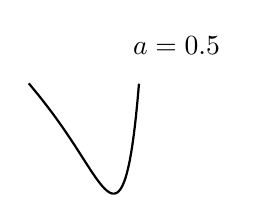
\begin{tikzpicture}[line join=round, scale=0.4]
\mydrawxy{-3}{3}{-2}{3}
\draw[thick,domain=-2:1.5,samples=200] plot (\x,{(0.5)*exp(2*\x)+(0.5-2)*exp(\x)-\x});
\coordinate[label=right:{$a=0.5$}] (t) at (1,3);
\end{tikzpicture}
\end{minipage}
\begin{minipage}{.32\textwidth}
\centering
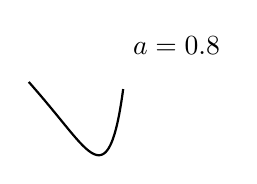
\begin{tikzpicture}[line join=round, scale=0.4]
\mydrawxy{-3}{3}{-2}{3}
\draw[thick,domain=-2:1,samples=200] plot (\x,{(0.8)*exp(2*\x)+(0.8-2)*exp(\x)-\x});
\coordinate[label=right:{$a=0.8$}] (t) at (1,3);
\end{tikzpicture}
\end{minipage}
\begin{minipage}{.32\textwidth}
\centering
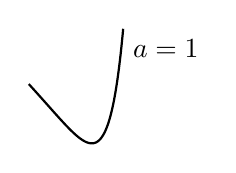
\begin{tikzpicture}[line join=round, scale=0.4]
\mydrawxy{-3}{3}{-2}{3}
\draw[thick,domain=-2:1,samples=200] plot (\x,{(1)*exp(2*\x)+(1-2)*exp(\x)-\x});
\coordinate[label=right:{$a=1$}] (t) at (1,3);
\end{tikzpicture}
\end{minipage}
\end{figure}

\begin{tcolorbox}
本题没有难度。函数形状的讨论都是针对其一阶和二阶导数的分段讨论,讨论的是另两个函数。
\end{tcolorbox}










\chapter{计数原理}

本章主要介绍排列组合。

本章要点:
\begin{itemize}
    \item 计数原理。
    \item 排列组合。
    \item 二项式定理。
\end{itemize}

\newpage
\section{分类加法计数原理与分步乘法计数原理}

本节要点:
\begin{itemize}
    \item 深刻理解和熟练掌握分类加法计数原理;
    \item 深刻理解和熟练掌握分步乘法计数原理。
\end{itemize}

~

本节是本章的基础,要熟练掌握。

分类加法计数原理体现的是空间上的并列性,步骤间相互独立;分步乘法计数原理体现了时间上的先后性,步骤间可能有相关性,后面几步的取值范围可能受上几步的影响。






\newpage
\section{排列与组合}

本节要点:
\begin{itemize}
    \item 掌握排列的概念及其计算公式;
    \item 掌握组合的概念及其计算公式。
\end{itemize}

~

\begin{definition}[排列和组合]
从$n$个元素中任取$m$个元素($m\leqslant n$)排成一有序列,称{\bf 从$n$个元素中取出$m$个元素的一个排列},所有排列的个数称作{\bf 排列数},记作$P_{n}^{m}$,有:
\[
P_{n}^{m}:=\frac{n!}{\left( n-m \right) !}=n\left( n-1 \right) \left( n-2 \right) \cdots \left[ n-\left( m-1 \right) \right]
\]
从$n$个元素中任取$m$个元素($m\leqslant n$)组成一无序组,称{\bf 从$n$个元素中取出$m$个元素的一个组合},所有组合的个数称作{\bf 组合数},记作$C_{n}^{m}$,有:
\[
C_{n}^{m}:=\frac{n!}{\left( n-m \right) !\cdot m!}=\frac{P_{n}^{m}}{m!}
\]
特别地,$P_{n}^{1}=C_{n}^{1}=n,P_{n}^{n}=n!,C_{n}^{n}=1$。
\end{definition}

排列组合均是对“从$n$个元素中抽取$m$个元素”的计算,排列突出有序,组合突出无序。排列组合的关系还可以这么理解,当$m$个元素排列完成后,若不考虑其顺序,就是组合,由于每个排列有$P_{m}^{m}$种不同的顺序,所以:
\[
P_{n}^{m}=C_{n}^{m}\cdot P_{m}^{m}=C_{n}^{m}\cdot m!
\]

\begin{theorem}
组合公式有以下性质:
\begin{align*}
&C_{n}^{m}=C_{n}^{n-m} \\
&C_{n+1}^{m}=C_{n}^{m}+C_{n}^{m-1}
\end{align*}
\end{theorem}






\newpage
\section{二项式定理}

本节要点:
\begin{itemize}
    \item 熟练掌握二项式定理。
\end{itemize}

~

\begin{align*}
\left( a+b \right) ^n=&C_{n}^{0}a^nb^0+C_{n}^{1}a^{n-1}b^1+\cdots + \\
&C_{n}^{k}a^{n-k}b^k+\cdots + \\
&C_{n}^{n-1}a^1b^{n-1}+C_{n}^{n}a^0b^n
\end{align*}






\newpage
\section{本章小结}

本章介绍了计数原理和排列组合,是后一章的基础,需要认真掌握。










\chapter{随机变量及其分布}

本章介绍随机变量。

本章要点:
\begin{itemize}
    \item 条件概率。
    \item 全概率公式。
    \item 离散型随机变量。
    \item 3类分布。
\end{itemize}

\newpage
\section{条件概率与全概率公式}

本节要点:
\begin{itemize}
    \item 掌握并理解条件概率的概念;
    \item 掌握并理解全概率公式;
    \item 深刻理解贝叶斯公式的哲学意义。
\end{itemize}

%============================================================
\subsection{条件概率}

\begin{definition}[条件概率]
在事件$A$发生的情况下,事件$B$发生的概率称为{\bf 条件概率},记作$P\left( B \middle| A \right) $,当$P\left( A \right) >0$时有:
\[
P\left( B \middle| A \right) := \frac{P\left( AB \right)}{P\left( A \right)}
\]
\end{definition}

\begin{tcolorbox}
$P\left( B \middle| A \right) $和$P\left( B \right) $的大小关系是不定的。
也就是说,事件$A$的发生并不一定有利于$B$,也可能没有影响。
切不能想当然地认为$P\left( B \middle| A \right) >P\left( B \right) $!
\end{tcolorbox}

\begin{theorem}[乘法公式]
若$P\left( A \right) >0$,则
\[
P\left( AB \right) =P\left( A \right) \left( B \middle| A \right)
\]
\end{theorem}

\begin{corollary}[乘法公式]
若$P\left( A_1A_2\cdots A_n \right) >0,n\geqslant 2$,则
\[
P\left( A_1A_2\cdots A_n \right) =P\left( A_1 \right) P\left( A_2 \middle| A_1 \right) P\left( A_3 \middle| A_1A_2 \right) \cdots P\left( A_n \middle| A_1A_2\cdots A_{n-1} \right)
\]
\end{corollary}

%============================================================
\subsection{全概率公式}

\begin{definition}[完备事件组]
若事件组$A_1,A_2,\cdots ,A_i,\cdots $两两互斥,且$A_1+A_2+\cdots +A_i+\cdots =\varOmega $,则$A_1,A_2,\cdots ,A_i,\cdots $构成样本空间$\varOmega $的一个{\bf 完备事件组},简称{\bf 完备组}。
\end{definition}

\begin{tcolorbox}
虽然教材上没提,但是我们还是需要理解完备组的概念,运用全概率的前提就是找到一个完备组。
\end{tcolorbox}

\begin{definition}[全概率公式]
若事件组$A_1,A_2,\cdots ,A_i,\cdots $构成样本空间$\varOmega $的一个完备组,则对于任何事件$B$有:
\[
P\left( B \right) =\sum_{i=1}^{\infty}{P\left( A_iB \right)}=\sum_{i=1}^{\infty}{\left[ P\left( A_i \right) \cdot P\left( B \middle| A_i \right) \right]}
\]
\end{definition}

完备组“瓜分”了整个样本空间,是事件对立关系的扩充,其意义在于将一个复杂的大问题分解为若干个简单的小问题。

全概率可以认为是条件概率的延申,如果事件组满足完备条件,则事件$B$的发生总是伴随某个组员的发生,或者说$B$是通过某个路径发生的。当$P\left( B \right) $的计算较为复杂时,我们可以构造一个合适的完备组,简化$P\left( B \right) $的计算。其次,该公式从数学上还可以理解为$P\left( B \right) $是$P\left( B \middle| A_i \right) $的加权和,权重为$P\left( A_i \right) $。最后还需注意,$P\left( B \right) \leqslant 1$,但$\sum_{i=1}^{\infty}{P\left( B \middle| A_i \right)}$几乎可能大于1。

\begin{tcolorbox}
全概率公式$P\left( B \right) =\sum_{i=1}^n{\left[ P\left( A_i \right) \cdot P\left( B \middle| A_i \right) \right]} $中,$P\left( B \middle| A_i \right) $可以认为是事件$B$在基$A_i$下的坐标分量,该分量越大,表示越可能发生。
\end{tcolorbox}

\begin{definition}[贝叶斯公式]
若事件$A_1,A_2,\cdots ,A_i,\cdots $构成样本空间$\varOmega $的一个完备事件组,且$P\left( A_i \right) >0$,若$B$为一随机事件,且$P\left( B \right) >0$,则:
\[
P\left( A_i \middle| B \right) =\frac{P\left( A_i \right) P\left( B \middle| A_i \right)}{\sum_{i=1}^{\infty}{\left[ P\left( A_i \right) \cdot P\left( B \middle| A_i \right) \right]}}=\frac{P\left( A_i \right) P\left( B \middle| A_i \right)}{P\left( B \right)}
\]
又称{\bf 逆概率公式}。通常,我们将$P\left( A_i \right) $称为{\bf 先验概率},将条件概率$P\left( A_i \middle| B \right) $称为{\bf 后验概率}。也可以结合向量内积理解。
\end{definition}

\begin{proof}
由条件概率的概念可得:
\[
P\left( A_i \middle| B \right) =\frac{P\left( A_iB \right)}{P\left( B \right)}
\]
结合全概率公式,且$P\left( A_iB \right) =P\left( BA_i \right) =P\left( A_i \right) P\left( B \middle| A_i \right) $。
\end{proof}

$P\left( A_i \right) $称为先验概率的原因是$A_i$作为一种假定而不依赖于$B$。$B$称为{\bf 证据},一种出现的客观事物。在证据出现前,$A_i$有自己的概率。当证据发现时,$A_i$的概率变成了$P\left( A_i \middle| B \right) $,所以我们称为后验概率。“先”和“后”指的是证据出现前和出现后。其中$P\left( B \middle| A_i \right) $描述了$A_i$和$B$的关系,机器学习中称为{\bf 似然(likehood)}。

全概率公式体现了由因求果,而贝叶斯公式反映了执果寻因的一种辩证思想,我们知道完备组员的概率$P\left( A_i \right) $和$B$在各个完备组员的条件概率$P\left( B \middle| A_i \right) $,就可以计算$B$大概会发生在哪个组员。很多情况下,我们知道各个原因发生的可能性,但是一旦结果出现,这些原因的可能性又会出现变化,贝叶斯公式揭示了两者之间的关系。

%============================================================
\subsection{习题}

\begin{example}[复习巩固3,难度:$\star $]
甲、乙两人向同一个目标各射击1次,已知甲命中目标的概率为0.6,乙命中目标的概率为0.5。已知目标至少被命中1次,求甲命中目标的概率。
\end{example}

解:

设甲命中目标为$A$,乙命中目标为$B$,目标至少被命中1次为$C$,由于甲乙相互独立,有:
\[
P\left( C \right) =P\left( A \right) +P\left( \bar{A}B \right) =P\left( A \right) +P\left( \bar{A} \right) \cdot P\left( B \right)
\]
甲命中目标的概率可表示为条件概率:
\begin{align*}
P\left( A \middle| C \right) &=\frac{P\left( AC \right)}{P\left( C \right)}=\frac{P\left( A \right) \cdot P\left( \bar{B} \right) +P\left( A \right) \cdot P\left( B \right)}{P\left( A \right) +P\left( \bar{A} \right) \cdot P\left( B \right)} \\
&=\frac{0.6\cdot 0.5+0.6\cdot 0.5}{0.6+0.4\cdot 0.5}=0.75
\end{align*}

拓展讨论:

$C$的概率可以有如下三种算法:
\begin{itemize}
    \item 甲命中乙不命中+甲不命中乙命中+甲乙都命中;
    \item 甲命中+甲不命中乙命中;
    \item 乙命中+乙不命中甲命中。
\end{itemize}
以上三种算法是三种完备组,易得这三种方法的结果是一样的。
\begin{align*}
P\left( C \right) &=P\left( A \right) +P\left( \bar{A}B \right) =P\left( A \right) +P\left( \bar{A} \right) \cdot P\left( B \right) \\
&=P\left( A \right) \cdot \left[ P\left( B \right) +P\left( \bar{B} \right) \right] +P\left( \bar{A} \right) \cdot P\left( B \right) \\
P\left( C \right) &=P\left( B \right) +P\left( \bar{B}A \right) =P\left( B \right) +P\left( \bar{B} \right) \cdot P\left( A \right) \\
&=P\left( B \right) \left[ P\left( A \right) +P\left( \bar{A} \right) \right] +P\left( \bar{B} \right) \cdot P\left( A \right) \\
P\left( C \right) &=P\left( A\bar{B} \right) +P\left( \bar{A}B \right) +P\left( AB \right) \\
&=P\left( A \right) \cdot P\left( \bar{B} \right) +P\left( \bar{A} \right) \cdot P\left( B \right) +P\left( A \right) \cdot P\left( B \right)
\end{align*}

\begin{tcolorbox}
本题关键在于理解$P\left( C \right) ,P\left( AC \right) $。
\end{tcolorbox}

~

\begin{example}[复习巩固4,难度:$\star $]
甲乙两个箱子中各装有10个球,其中甲箱中有5个红球、5个白球,乙箱中有8个红球、2个白球。掷一枚质地均匀的骰子,如果点数为1或2,从甲箱子中随机摸出1个球;如果点数为3,4,5,6,从乙箱子中随机摸出1个球。
求摸到红球的概率。
\end{example}

解:

设骰子点数为1或2为$A$,从甲箱子中摸出红球为$B$,从乙箱子中摸出红球为$C$,则:
\begin{align*}
P&=P\left( A \right) \cdot P\left( \bar{B} \right) +P\left( A \right) \cdot P\left( C \right) \\
&=\frac{2}{6}\cdot \frac{5}{10}+\frac{4}{6}\cdot \frac{8}{10}=\frac{7}{10}
\end{align*}

拓展讨论:

红球要么从甲箱要么从乙箱中获得,构成一个完备组,而骰子的出现可以认为是给甲箱和乙箱加了一个加权系数,而且加权系数和为1。

\begin{tcolorbox}
本题运用全概率公式即可。
\end{tcolorbox}

~

\begin{example}[复习巩固5,难度:$\star $]
在A,B,C三个地区爆发了流感,这三个地区分别有6\%,5\%,4\%的人患了流感。假设这三个地区的人口数的比为5:7:8,现从这三个地区中任意选取一个人。
\begin{enumerate}
    \item 求这个人患流感的概率;
    \item 如果此人患流感,求此人选自A地区的概率。
\end{enumerate}
\end{example}

解:

显然地区A、B、C构成完备组。

(1)
\[
P\left( A \right) =\frac{5}{5+7+8}\cdot 6\%+\frac{7}{5+7+8}\cdot 5\%+\frac{8}{5+7+8}\cdot 4\%=4.85\%
\]

(2)
\[
P=\frac{\frac{5}{5+7+8}\cdot 6\%}{P\left( A \right)}=\frac{0.015}{0.0485}=0.309278
\]

\begin{tcolorbox}
本题考查条件概率,不难。
\end{tcolorbox}

~
\begin{example}[综合运用7,难度:$\star $]
一批产品共有100件,其中5件为不合格品。收货方从中不放回地随机抽取产品进行检验,并按以下规则判断是否接受这批产品:如果抽检的第1件产品不合格,则拒绝整批产品;如果抽检的第1件产品合格,则再抽1件,如果抽检的第2件产品合格,则接受整批产品,否则拒绝整批产品。求这批产品被拒绝的概率。
\end{example}

解:

易得,这批产品要么整批接收,要么整批拒绝,显然整批接收的条件为两次抽检均合格,比较好计算,有:
\[
1-P\left( A \right) =1-\frac{95}{100}\cdot \frac{94}{99}=0.0979798
\]

\begin{tcolorbox}
本题用补集清晰简单。
\end{tcolorbox}

%============================================================
\subsection{拓展习题}

\begin{example}
设10件产品中存在2件次品,现不放回地抽取2次,每次1件,求第2件是次品的概率。
\end{example}

解:

显然第2件是否为次品和第1件为否是次品有关,是典型的条件概率。更进一步,第1件产品的合格和次品两个事件可以构成完备组,所以可以用全概率公式求解。

设第1次抽取为次品为事件$A$,于是$A,\bar{A}$可视为完备组,且易得$P\left( A \right) =\frac{2}{10},P\left( \bar{A} \right) =\frac{8}{10}$。再设第2次抽到次品为事件$B$,于是$P\left( B \right) $可以用这个完备组分解:
\[
P\left( B \right) =P\left( A \right) P\left( B \middle| A \right) +P\left( \bar{A} \right) P\left( B \middle| \bar{A} \right)
\]
其中:
\begin{itemize}
    \item $P\left( B \middle| A \right) $:表示第1次抽到次品时第2次也抽到次品的概率,易得$\frac{1}{9}$;
    \item $P\left( B \middle| \bar{A} \right) $:表示第1次抽到合格时第2次抽到次品的概率,易得$\frac{2}{9}$。
\end{itemize}
最终得到:
\[
P\left( B \right) =\frac{1}{5}\cdot \frac{1}{9}+\frac{4}{5}\cdot \frac{2}{9}=\frac{1}{5}
\]

解二,不用全概率的概念,直接使用古典概型的方法,抽取2件排序,共$P_{10}^{2}$种,第2件是次品有两种互不相同可能:
\begin{itemize}
    \item 第1次抽到次品时第2次也抽到次品,$C_{2}^{1}\cdot C_{1}^{1}$种;
    \item 第1次抽到合格时第2次抽到次品,$C_{8}^{1}\cdot C_{2}^{1}$种。
\end{itemize}
于是:
\[
P=\frac{C_{2}^{1}\cdot C_{1}^{1}+C_{8}^{1}\cdot C_{2}^{1}}{P_{10}^{2}}=\frac{18}{90}=\frac{1}{5}
\]

~

\begin{example}
假设血清甲蛋白法测定肝癌阳性准确率为95\%、阴性准确率为90\%,若已知社会人群的患癌率为0.04\%,若某人检测阳性,分析其实际患癌的概率。
\end{example}

解:

设事件$A$表示被检者实际患癌,事件$B$ 表示用该测定法判定阳性,由题干可知:
\begin{align*}
&P\left( A \right) =0.0004 \\
&P\left( B \middle| A \right) =0.95 \\
&P\left( \bar{B} \middle| \bar{A} \right) =0.90
\end{align*}
由于$A,\bar{A}$构成完备组,则有:
\begin{align*}
P\left( A \middle| B \right) &=\frac{P\left( A \right) P\left( B \middle| A \right)}{P\left( A \right) P\left( B \middle| A \right) +P\left( \bar{A} \right) P\left( B \middle| \bar{A} \right)} \\
&=\frac{0.0004\cdot 0.95}{0.0004\cdot 0.95+0.9996\cdot \left( 1-0.9 \right)} =0.00378712
\end{align*}

一方面可见即便测定阳性,实际患癌也不到1\%,但比一般人群已经高了$0.3787/0.04=9.4675$,将近10倍。另一方面,通过贝叶斯公式我们了解到,血清甲蛋白测定法不是判断患癌的概率,而是判断比正常人患癌概率高了多少。

\begin{tcolorbox}
该例子很具典型性。首先0.04\%的患癌概率是作为一种先天的经验存在。测试结果则是一种证据。证据的出现可以让我们对这个先天经验进行修正。由于这个证据本身带有概率,而非100\%,所以它实际上是提高了患癌概率。
\end{tcolorbox}

~

\begin{example}
某水文站测量水流量,令$B$为测量不准的事件,并总结了几个测量不准的原因$A_i$,原因的发生概率$P\left( A_i \right) $,以及某个原因发生时测量不准的概率$P\left( B \middle| A_i \right) $,如下表,分析哪几个原因主要导致了测量不准。
\begin{table}[h]
    \centering
    \begin{tabular}{cccc}
        \toprule
        测不准的原因$A_i$ & $P\left( A_i \right) $ & $P\left( B \middle| A_i \right) $ & $P\left( A_i \middle| B \right) $\\
        \midrule
        流速计故障 & 0.01 & 0.90 & 0.05\\
        绕道设备误差 & 0.05 & 0.80 & 0.24\\
        水中有杂质 & 0.04 & 0.10 & 0.02\\
        气象条件不佳 & 0.10 & 0.30 & 0.18\\
        人员配合问题 & 0.10 & 0.80 & 0.47\\
        其他 & 0.70 & 0.01 & 0.04\\
        \bottomrule
    \end{tabular}
\end{table}
\end{example}

解:

“那几个原因主要导致了测量不准”也即测量不准的情况下,各个原因的发生概率$P\left( A_i \middle| B \right) $,可以用贝叶斯公式解决。
\[
P\left( A_i \middle| B \right) =\frac{P\left( A_i \right) P\left( B \middle| A_i \right)}{P\left( B \right)}=\frac{P\left( A_i \right) P\left( B \middle| A_i \right)}{\sum_{i=1}^{\infty}{P\left( A_i \right) P\left( B \middle| A_i \right)}}
\]
计算结果如上表最右列。可见,单看每个已知的明确的原因,它们的发生概率都不大,但是一旦问题出现,最有可能是人员配合导致。所以若要提高测量准确度,首先得从提高人员配合度着手。

~

\begin{example}
甲箱中有2个白球4个黑球,乙箱中有6个白球2个黑球,现从这两箱中各任取一球,再从所取出的两球中任取一球,求最终该球是白球的概率。
\end{example}

解:

令从甲箱中取得白球为事件$A$,从乙箱中取得白球为事件$B$,易得甲乙两个箱子中取球为独立事件,于是:
\begin{align*}
&P\left( A \right) =\frac{1}{3},P\left( B \right) =\frac{3}{4} \\
&P\left( AB \right) =\frac{1}{4},P\left( A\bar{B} \right) =\frac{1}{12},P\left( \bar{A}B \right) =\frac{1}{2},P\left( \bar{A}\bar{B} \right) =\frac{1}{6}
\end{align*}
且$AB,\bar{A}B,A\bar{B},\bar{A}\bar{B}$构成完备组,于是可以用全概率公式得到:
\begin{align*}
P\left( C \right) =&P\left( AB \right) P\left( C \middle| AB \right) +P\left( A\bar{B} \right) P\left( C \middle| A\bar{B} \right) + \\
&P\left( \bar{A}B \right) P\left( C \middle| \bar{A}B \right) +P\left( \bar{A}\bar{B} \right) P\left( C \middle| \bar{A}\bar{B} \right)
\end{align*}
而易得:
\begin{align*}
&P\left( C \middle| AB \right) =1 \\
&P\left( C \middle| A\bar{B} \right) =P\left( C \middle| \bar{A}B \right) =\frac{1}{2} \\
&P\left( C \middle| \bar{A}\bar{B} \right) =0
\end{align*}
于是:
\[
P\left( C \right) =\frac{1}{4}+\frac{1}{12}\cdot \frac{1}{2}+\frac{1}{2}\cdot \frac{1}{2}=\frac{13}{24}
\]






\newpage
\section{离散型随机变量及其分布列}

本节要点:
\begin{itemize}
    \item 掌握一维离散型随机变量及其分布律的概念;
    \item 掌握0-1分布的概念。
\end{itemize}

~

\begin{definition}[一维随机变量]
设随机试验$E$的样本空间为$\varOmega $,若每个样本点$\omega$均有唯一确定的实数$X$与之对应,则称$X$为{\bf 定义在$\varOmega $上的一维随机变量},也称{\bf 随机变量}或简称{\bf 变量}。
\end{definition}

随机变量将对样本点的文字描述投射到实数,注意,这里投射的是样本点,或者说是基本事件,而非任意事件。$X$的值在有些情况下可直观地赋予,如次品数量、人流数量、等待时间,但在有些情况下是人为赋予的,并没有特别的物理意义,如抛硬币的正反面,此时只要保证“唯一”、“确定”两个要求即可。

于是,我们将事件$A$及其概率$P\left( A \right) $和变量$X$的取值范围$D$的概率$P\left\{ X\in D \right\} $等价起来:
\[
\begin{array}{l}
	\omega\\
	A\\
	P\left( A \right)\\
\end{array}\Leftrightarrow \begin{array}{l}
	X\\
	X\in D\\
	P\left\{ X\in D \right\}\\
\end{array}
\]
一维随机变量可视作一种特殊的变量,虽然其取值范围可以为$\mathbb{R} $,但与普通变量相比有如下特殊性:
\begin{itemize}
    \item 根据具体试验,随机变量有意义的取值是人为设定且事先已知的;
    \item 但是在试验前,具体的取值无法预知;
    \item 我们能知道的是每个取值的概率。
\end{itemize}

\begin{definition}[分布函数]
设有随机变量$X$,对于$\forall x\in \mathbb{R} $,若$P\left\{ X\leqslant x \right\} $均有唯一的值与之对应,则称该对应关系为{\bf $X$的分布函数},记作$F\left( x \right) $,即:
\[
F\left( x \right) := P\left\{ X\leqslant x \right\} ,\qquad x\in \mathbb{R}
\]
\end{definition}

分布函数描述了$X$每个取值之前(包括该值)的所有概率之和,所以分布函数的差可以描述变量在一个范围内的概率,即$X$在$\left( a,b \right] $的概率可以表示为:
\[
P\left\{ a<X\leqslant b \right\} =F\left( b \right) -F\left( a \right)
\]
分布函数的定义还隐含了判断一个函数能否被视为分布函数的充要条件:
\[
F\left( X \right) \text{是分布函数}\Leftrightarrow \begin{cases}
	0\leqslant F\left( x \right) \leqslant 1\\
	\underset{x\rightarrow -\infty}{\lim}F\left( x \right) =P\left( \oslash \right) =0\\
	\underset{x\rightarrow +\infty}{\lim}F\left( x \right) =P\left( \varOmega \right) =1\\
\end{cases}
\]
分布函数还有以下性质:
\begin{itemize}
    \item $F\left( x \right) $必单调增,即$x_1<x_2\Rightarrow F\left( x_1 \right) \leqslant F\left( x_2 \right) $;
    \item $F\left( x \right) $每个点$x_0$均右连续,即$\underset{x\rightarrow {x_0}^+}{\lim}F\left( x \right) =F\left( x_0 \right) $。
\end{itemize}

这里需要理解$X,x$两者的区别。$x$是普通变量,取值范围为$\mathbb{R} $,本身不承担物理意义,而$X$是随机变量,有意义的取值范围通过事件规定。如投硬币中,我们规定$X=1$表示正面向上,$X=0$表示反面向上,$X$取0、1之外的值是没有意义的,或者说$P\left\{ X\ne 0\mathrm{or}1 \right\} =0$。

至此,我们将之前的概念和函数的概念统一了起来,我们用变量代替样本,用函数描述概率。
\begin{table}[h]
\centering
\begin{tabular}{ll}
    \toprule
    \multicolumn{1}{c}{事件} & \multicolumn{1}{c}{变量}  \\
    \midrule
    样本点$\omega $ & 随机变量$X$\\
    样本空间$\varOmega $ & $\mathbb{R} $\\
    随机事件$A$ & 取值范围,如$\left\{ X=1 \right\} ,\left\{ X\geqslant b \right\} ,\left\{ a<X\leqslant b \right\} $\\
    概率$P\left( A \right) $ & 分布函数的差,如$P\left\{ a<X\leqslant b \right\} =F\left( b \right) -F\left( a \right) $\\
    \bottomrule
\end{tabular}
\end{table}

\begin{definition}[一维离散型随机变量]
若一维随机变量$X$的取值为有限个或可列无穷多个,则称$X$为{\bf 一维离散型随机变量},简称{\bf 离散变量}。设可能的取值为$x_1,x_2,\cdots ,x_i,\cdots $,且对应的概率记作:
\[
P\left\{ X=x_i \right\} =p_i
\]
称序列$p_i$为$X$的{\bf 分布律}或{\bf 概率分布},可用表格展现,或记作:
\[
X\sim \left( \begin{matrix}
	x_1&		x_2&		\cdots&		x_i&		\cdots\\
	p_1&		p_2&		\cdots&		p_i&		\cdots\\
\end{matrix} \right)
\]
其中:
\begin{itemize}
    \item $x_i$:纯数学记号,对应基本事件$A_i$,通常为简化讨论,$x_i$取值为非负整数,分布律的计算通常基于上一章的讨论;
    \item $p_i=P\left\{ X=x_i \right\} =P\left( A_i \right) $:表示基本事件$A_i$的发生概率。
\end{itemize}
\end{definition}

若离散变量$X$有分布律$p_i$,则其分布函数为:
\[
F\left( x \right) =P\left\{ X\leqslant x \right\} =\sum_{x_i\leqslant x}{p_i}
\]
由分布函数的充要条件可得$p_i$成为分布律的充要条件:
\[
p_i\text{为分布律}\Leftrightarrow \begin{cases}
	p_i\geqslant 0\\
	\sum_i{p_i}=1\\
\end{cases}
\]

~

{\bf 0-1分布}又称{\bf 两点分布},记作$B\left( 1,p \right) $,描述最简单的分布:
\begin{align*}
&P\left\{ X=1 \right\} =p\\
&P\left\{ X=0 \right\} =1-p
\end{align*}
更普遍地记作:
\[
P\left\{ X=x \right\} =p^x\left( 1-p \right) ^{1-x},\qquad \begin{array}{l}
	x=0,1\\
	p\in \left( 0,1 \right)\\
\end{array}
\]
其中:
\begin{itemize}
    \item $x$:一般取0表示事件不发生,1表示事件发生;
    \item $p$:表示事件发生的概率。
\end{itemize}
特别地,当$p=0\mathrm{or}1$时称为{\bf 常数分布}。常数分布表示了事件100\%发生,所以无实际用途,只是为了完善概念而提出。

\begin{tcolorbox}
一般如果试验中只有两个样本点,非黑即白、非正即负,我们就可以用两点分布描述。两点分布的使用场景非常少。
\end{tcolorbox}

%============================================================
\subsection{拓展讨论:密度函数的物理意义}

\begin{tcolorbox}
离散变量的分布律的意义是清晰的,每个点代表基本事件的发生概率。但连续变量的密度函数的意义并不十分清晰,本节讨论密度函数的物理意义,以求能直观地把握这个概念。
\end{tcolorbox}

若有一维无限长细线,总质量为$M$但分布不均匀,已知线密度$\rho \left( l \right) $,$l$为距原点的距离,任取一段$\left[ l_1,l_2 \right] $,该段质量占比为:
\[
\frac{m}{M}=\int_{l_1}^{l_2}{\frac{\rho \left( l \right)}{M}\cdot dl}
\]

若考虑一维无限长带电细线,总电荷量为$Q$但分布不均匀,已知电密度$\rho \left( l \right) $,任取一段$\left[ l_1,l_2 \right] $,该段电荷占比为:
\[
\frac{q}{Q}=\int_{l_1}^{l_2}{\frac{\rho \left( l \right)}{Q}\cdot dl}
\]

再考虑变速运动,若速度随时间变化且有规律$v=v\left( t \right) $,则在某时段走过的路程占总路程$S$:
\[
\frac{s}{S}=\int_{t_1}^{t_2}{\frac{v\left( t \right)}{S} \cdot dt}
\]

对比概率计算公式:
\[
P\left\{ a<X\leqslant b \right\} =\int_a^b{f\left( x \right) \cdot dx}
\]
容易发现,概率$P\left\{ a<X\leqslant b \right\} $表示了一段范围内某个物理量的占比,密度函数$f\left( x \right) $刻画了该物理量的分布情况。根据$\rho \left( l \right) $我们可以知道哪里重,根据$v \left( t \right) $我们可以知道哪个时段走得多。同样道理,根据密度函数,我们可以知道$X$在哪里出现的概率大。关联到具体事件,我们就可以知道哪些事件容易发生。所以,我们通常用“占比大”、“出现多”来指代概率大。

~

{\bf 密度函数的物理意义是反映了一个物理量在某个范围内的占比。}这个“占比”就是概率,而“范围”可以是空间上的一个段,也可以是时间上的一个段。以质量为例,可以认为密度函数具有量纲$\left[ \mathrm{m}^{-1} \right] $。






\newpage
\section{离散型随机变量的数字特征}

本节要点:
\begin{itemize}
    \item 掌握数学期望的概念;
    \item 理解数学期望的数学意义和物理意义;
    \item 掌握方差的概念;
    \item 理解方差的统计意义和物理意义。
\end{itemize}

%============================================================
\subsection{离散型随机变量的均值}

\begin{definition}[数学期望]
设离散变量$X$有分布律$p_i$,若无穷级数$\sum_{i=1}^{+\infty}{x_i\cdot p_i}$绝对收敛(即$\sum_{i=1}^{+\infty}{\left| x_i\cdot p_i \right|}$收敛),则称该无穷级数为$X$的{\bf 数学期望}或{\bf 均值},记作$E\left( X \right) $或$EX$:
\[
EX:=\sum_{i=1}^{+\infty}{x_i\cdot p_i}
\]
若离散变量取值为有限个,则必有数学期望。
\end{definition}

一般,我们用$E\left( X \right) $表示谓词,即计算$X$的数学期望这个过程,用$EX$表示名词,即数学期望这个值。$E$是Expectation的首字母。

\begin{tcolorbox}
级数有个现象,如果调换各项的顺序,收敛性可能发生改变,即便收敛,也可能收敛到不同的值,而在概率论中,随机变量的取值和顺序无关,所以这里要求绝对收敛。
\end{tcolorbox}


\begin{definition}[随机变量函数的数学期望]
设离散变量$X$有分布律$p_i$,若有另一随机变量$Y=g\left( X \right) $,且无穷级数$\sum_{i=1}^{+\infty}{g\left( x_i \right) p_i}$绝对收敛,则称$E\left[ g\left( X \right) \right] $为{\bf 函数$Y=g\left( X \right) $的数学期望}:
\[
EY:=\sum_{i=1}^{+\infty}{g\left( x_i \right) \cdot p_i}
\]
\end{definition}

该公式的意义在于,有时候我们很难获得$Y$的具体分布规律,但可以通过已知的$X$和$Y=g\left( X \right) $获得$Y$的数学期望。

%============================================================
\subsection{离散型随机变量的方差}

\begin{definition}[方差]
设离散型随机变量$X$,若函数$\left( X-EX \right) ^2$的数学期望存在,则称该数学期望为$X$的{\bf 方差},记作$D\left( X \right) $或$DX$,即:
\[
DX:=E\left[ \left( X-EX \right) ^2 \right] =\sum_{i=1}^{+\infty}{\left( x_i-EX \right) ^2\cdot p_i}
\]
同时称$\sqrt{DX}$为{\bf $X$的平方差}。
\end{definition}

\begin{tcolorbox}
方差的英文为Variance,有些教材使用$\mathrm{Var}\left( X \right) $作为记号。
\end{tcolorbox}

方差的求解较为繁琐,由于$\left( X-EX \right) ^2=X^2-2\cdot X\cdot EX+\left( EX \right) ^2$,且$EX$是常数,利用数学期望的性质可得便捷公式:
\begin{align*}
DX&=E\left[ X^2-2\cdot X\cdot EX+\left( EX \right) ^2 \right] \\
&=E\left( X^2 \right) -2\cdot EX\cdot EX+\left( EX \right) ^2 \\
&=E\left( X^2 \right) -\left( EX \right) ^2
\end{align*}

从便捷公式可以得到$\left[ E\left( X \right) \right] ^2$和$E\left( X^2 \right) $的关系:
\[
E\left( X^2 \right) =DX+\left( EX \right) ^2
\]
由于$DX\geqslant 0$,所以$E\left( X^2 \right) \geqslant \left( EX \right) ^2$。

\begin{tcolorbox}
由于数学期望的线性性,便捷公式的推导没有任何前置条件,所以被广泛使用,定义式则更多用来理解概念。
\end{tcolorbox}

%============================================================
\subsection{拓展讨论:数学期望的数学意义}

数学期望是随机变量的加权和,权重是概率,由于总概率为1,于是$EX<x_{+\infty}$,所以期望也称加权平均。任何一个给定的随机变量,若有数学期望,则都是一个固定的、可计算的常量。

从线性代数看,数学期望是随机变量构成的向量及其分布规律构成的向量的标量积。以离散型随机变量为例:
\begin{align*}
&EX:=\sum_{i=1}^{+\infty}{x_ip_i}=\boldsymbol{x}^T\boldsymbol{p} \\
&\begin{cases}
	\boldsymbol{x}=\left( x_1,x_2,\cdots ,x_n,\cdots \right)\\
	\boldsymbol{p}=\left( p_1,p_2,\cdots ,p_n,\cdots \right)\\
\end{cases}
\end{align*}
$EX$越大表示$\boldsymbol{p}$和$\boldsymbol{x}$的契合度越高,或者说越靠后的事件越容易发生。

\begin{tcolorbox}
这里的数学意义更多是为意义而意义,是一个“形象的比喻”,不用太过深究。
\end{tcolorbox}

%============================================================
\subsection{拓展讨论:数学期望的物理意义}

考虑一维物体的转动。长度为$L$的细长杆质量$M$且分布不均匀,有线密度$\rho \left( x \right) ,x\in \left[ d,d+L \right] $,一端距原点$d$,绕原点匀速转动且有角速度$\omega $,分析所需的向心力。可以认为是同质量的质点在$x_0$处以通常角速度转动所需的向心力。

可以假设细长杆的一个微元可视为质点,则向心力微元和整体向心力:
\begin{align*}
&dF=\rho \left( x \right) dx\cdot \omega ^2\cdot x\quad \left[ \mathrm{N} \right] \\
&F=\int_d^{d+L}{dF}=\int_d^{d+L}{\rho \left( x \right) dx\cdot \omega ^2\cdot x}=\omega ^2\int_d^{d+L}{x\rho \left( x \right) \cdot dx}\quad \left[ \mathrm{N} \right]
\end{align*}
若将其视为质点,则向心力等价为质量$M$的质点小球在$x_0$处以角速度$\omega $匀速转动,有:
\[
\omega ^2\int_d^{d+L}{x\rho \left( x \right) \cdot dx}=M\cdot \omega ^2\cdot x_0\quad \left[ \mathrm{N} \right]
\]
于是可得:
\[
x_0=\frac{\int_d^{d+L}{x\rho \left( x \right) \cdot dx}}{M}=\int_d^{d+L}{x\frac{\rho \left( x \right)}{M}\cdot dx}\quad \left[ \mathrm{m} \right]
\]
对比一维变量的数学期望定义式:
\[
EX=\int_{-\infty}^{+\infty}{xf\left( x \right) \cdot dx}
\]
{\bf 数学期望的物理意义为绕原点匀速转动时的质心位置,有量纲$\left[ \mathrm{m} \right] $}。

%============================================================
\subsection{拓展讨论:数学期望的性质}

{\bf 性质1}:常数的数学期望为其本身,即$E\left( c \right) =c$。

{\bf 性质2}:$X\geqslant a\Rightarrow EX\geqslant a,X\leqslant a\Rightarrow EX\leqslant a$

{\bf 性质3}:$E\left( kX \right) =k\cdot E\left( X \right) $

{\bf 性质4}:$E\left( kX+c \right) =k\cdot E\left( X \right) +c$,由性质1+3可证。

{\bf 性质5}:设$\left( X,Y \right) $为二维随机变量,则$E\left( X\pm Y \right) =E\left( X \right) \pm E\left( Y \right) $

{\bf 性质6}:设$\left( X,Y \right) $为二维随机变量,若$X,Y$相互独立$\Rightarrow E\left( XY \right) =E\left( X \right) \cdot E\left( Y \right) $

{\bf 性质7}:设$\left( X,Y \right) $为二维随机变量,则$\left[ E\left( XY \right) \right] ^2\leqslant E\left( X^2 \right) \cdot E\left( Y^2 \right) $

~

性质1表示了常数$c$的分布,其实就是质点小球,自然质心位置为$c$。

性质2表示了质心的范围,物理意义也很明显,质心位置肯定不会落到物体之外。

性质3表达当{\it x}轴拉伸时,质心也有同样的拉伸,压缩亦然。

\begin{tcolorbox}
这三个性质可结合物理意义理解。
\end{tcolorbox}

性质5用定义即可证明:
\begin{align*}
E\left( X\pm Y \right) &=\sum_{i=1}^{+\infty}{\sum_{j=1}^{+\infty}{\left( x_i\pm y_j \right) \cdot p_{ij}}}=\sum_{i=1}^{+\infty}{\sum_{j=1}^{+\infty}{\left( x_ip_{ij}\pm y_jp_{ij} \right)}} \\
&=\sum_{i=1}^{+\infty}{\sum_{j=1}^{+\infty}{x_ip_{ij}}}\pm \sum_{i=1}^{+\infty}{\sum_{j=1}^{+\infty}{y_jp_{ij}}} \\
&=E\left( X \right) \pm E\left( Y \right)
\end{align*}

性质6,独立则有$p_{ij}=p_{i\cdot}\cdot p_{\cdot j}$,于是:
\begin{align*}
E\left( XY \right) &=\sum_{i=1}^{+\infty}{\sum_{j=1}^{+\infty}{\left( x_iy_j \right) \cdot p_{ij}}}=\sum_{i=1}^{+\infty}{\sum_{j=1}^{+\infty}{\left( x_iy_j \right) \cdot p_{i\cdot}\cdot p_{\cdot j}}} \\
&=\sum_{i=1}^{+\infty}{\left( x_ip_{i\cdot}\cdot \sum_{j=1}^{+\infty}{y_jp_{\cdot j}} \right)}=\sum_{i=1}^{+\infty}{\left[ x_ip_{i\cdot}\cdot E\left( Y \right) \right]} \\
&=E\left( X \right) \cdot E\left( Y \right)
\end{align*}

\begin{tcolorbox}
数学期望的性质常用于随机变量组合成新变量的数学期望的计算。由于数学期望是线性运算,所以有
\[
E\left( aX+bY+c \right) =aEX+bEY+c
\]
但对于非线性组合,会有一些前置条件或者为不等式。
\end{tcolorbox}

\begin{tcolorbox}
$\left( EX \right) ^2$不大于$E\left( X^2 \right) $,证明关系留到介绍方差后再给出。
\end{tcolorbox}

%============================================================
\subsection{拓展讨论:数学期望的范围}

数学期望的范围是变量的范围,这点从数学期望的物理意义也很好理解,特别是当变量的分布为常数分布时,取到最大值。此时,随机事件变成确定性事件。对应地,函数的数学期望的范围是函数的值域。

%============================================================
\subsection{拓展讨论:中位数的概念}

\begin{definition}[中位数]
若随机变量$X$有分布函数$F\left( x \right) $,若$m$满足
\[
F\left( m \right) =\frac{1}{2}
\]
则称$m$为{\bf 随机变量$X$的中位数}。
\end{definition}

数学期望和中位数都反映了随机变量的一个均值情况。中位数表示了该点前后的概率是一样的,优点是受特大值、特小值影响小,而且必然存在,缺点是处理不方便(如两个随机变量加减乘除后的中位数),而且不唯一,特别在离散型随机变量,由于取值的离散型,中位数大多不会精确的存在。

从物理意义上理解,数学期望反映的是质心,考虑了质点的力矩,而中位数不考虑力矩的影响。

与中位数相关的还有一个概念,上侧$\alpha $分位点。

%============================================================
\subsection{拓展讨论:方差的数学由来和统计意义}

方差定义中,$X-EX$是根本,表示了随机变量$X$和它的均值$EX$的偏离程度。由于$E\left( X-EX \right) =E\left( X \right) -EX=0$,总是为0,所以我们取绝对值$\left| X-EX \right|$,又由于绝对值函数在0点不可导,所以我们替换成平方$\left( X-EX \right) ^2$定义方差。

方差描述了随机变量$X$偏离其数学期望的程度,$DX$越小,说明离散程度越小。

%============================================================
\subsection{拓展讨论:方差的物理意义}

考虑一维物体的转动。长度为$L$的细长杆质量$M$且分布不均匀,有线密度$\rho \left( x \right) ,x\in \left[ d,d+L \right] $,一端距原点$d$,绕原点转动。

其转动惯量$I$有:
\[
I=\int{x^2\cdot dM}=\int_d^{d+L}{x^2\cdot \rho \left( x \right) \cdot dx} \quad \left[ \mathrm{kg}\cdot \mathrm{m}^2 \right]
\]
若将转轴移到质心$x_0$ ,根据平行轴定理,新的转动惯量$I_{x_0}$有:
\begin{align*}
&\because I=I_{x_0}+{Mx_0}^2 \\
&\therefore \int_d^{d+L}{x^2\cdot \rho \left( x \right) \cdot dx}=I_{x_0}+{Mx_0}^2 \\
&\therefore \int_d^{d+L}{x^2\cdot \frac{\rho \left( x \right)}{M}\cdot dx}=\frac{I_{x_0}}{M}+{x_0}^2
\end{align*}
对比方差的便捷计算公式:
\[
E\left( X^2 \right) =\int_{-\infty}^{+\infty}{x^2f\left( x \right) \cdot dx}=DX+\left( EX \right) ^2
\]
显然,{\bf 方差的物理意义可以理解为物体以质心为原点时的单位质量的转动惯量,有量纲$\left[ \mathrm{m}^2 \right] $}。跟物理的转动惯量不一样,没有质量这个因子,所以描述的是一种和具体质量无关的惰性,这种惰性和分布有关,$DX$越大,说明分布越靠外,转动惯量也越大。

%============================================================
\subsection{拓展讨论:方差的性质}

{\bf 性质1}:常数的方差为0,即$D\left( c \right) =0$。

{\bf 推论}:$D\left( X \right) \geqslant 0$,当且仅当$P\left\{ X=EX \right\} =1$时(即常数分布),等号成立。

{\bf 性质2}:$D\left( kX \right) =k^2\cdot DX$

{\bf 性质3}:$D\left( kX+c \right) =k^2\cdot DX$,由性质1,2可得。

{\bf 性质4}:设$\left( X,Y \right) $为二维随机变量,

若$X,Y$相互独立$\Rightarrow D\left( X\pm Y \right) =DX+DY$

进一步地,若$X,Y$相互独立$\Rightarrow D\left( aX\pm bY \right) =a^2\cdot DX+b^2\cdot DY$

~

性质1,对于常数分布,质心就是$c$,显然绕质心的转动惯量为0。

性质2,若$X\rightarrow kX$,相当于直线被拉长$k$倍,自然转动惯量扩大了$k^2$倍。

\begin{tcolorbox}
上述性质可结合物理意义理解。
\end{tcolorbox}

性质4,证明如下:
\begin{align*}
&\because DX=E\left( X^2 \right) -\left( EX \right) ^2 \\
&\begin{aligned}
	\therefore D\left( X\pm Y \right) &=E\left[ \left( X\pm Y \right) ^2 \right] -E\left[ \left( X\pm Y \right) \right] \cdot E\left[ \left( X\pm Y \right) \right]\\
	&=E\left[ X^2\pm 2XY+Y^2 \right] -\left[ EX\pm EY \right] ^2\\
	&=\left[ E\left( X^2 \right) \pm 2E\left( XY \right) +E\left( Y^2 \right) \right] -\\
	&\left[ \left( EX \right) ^2\pm 2\left( EX \right) \left( EY \right) +\left( EY \right) ^2 \right]\\
\end{aligned} \\
&\because E\left( XY \right) =\left( EX \right) \left( EY \right) \\
&\begin{aligned}
	\therefore D\left( X\pm Y \right) &=\left[ E\left( X^2 \right) -\left( EX \right) ^2 \right] +\left[ E\left( Y^2 \right) -\left( EY \right) ^2 \right]\\
	&=DX+DY\\
\end{aligned}
\end{align*}

%============================================================
\subsection{拓展讨论:方差的取值范围}

变量的方差的取值范围根据不同的分布有不同的范围。如常数分布,中心点转动惯量必然为0。又如$P\left\{ X=\pm \infty \right\} =0.5$,显然转动惯量$+\infty $ 。

%============================================================
\subsection{拓展讨论:随机变量的标准化}

\begin{definition}[随机变量的标准化]
设随机变量$X$有数学期望$EX$和方差$DX>0$,若将$X$进行运算$\frac{X-EX}{\sqrt{DX}}$,获得的随机变量称为{\bf $X$的标准化随机变量},记作$X^*$,即:
\[
X^*=\frac{X-EX}{\sqrt{DX}}
\]
且有:
\begin{align*}
&E\left( X^* \right) =E\left( \frac{X-EX}{\sqrt{DX}} \right) =\frac{1}{\sqrt{DX}}\cdot E\left( X-EX \right) =0 \\
&D\left( X^* \right) =D\left( \frac{X-EX}{\sqrt{DX}} \right) =\frac{1}{DX}\cdot D\left( X-EX \right) =1
\end{align*}
\end{definition}

~

考察标准化过程:
\begin{itemize}
    \item $X-EX$:表示将坐标原点拉到期望$EX$的位置,即原点对称;
    \item $\frac{1}{\sqrt{DX}}$:拉伸或收缩{\it x}轴,使得分布不过于稀疏或稠密。
\end{itemize}
排除这两个“干扰”后,很多初看起来不同的分布,实际是一类分布,有利于后续的进一步分析。如不同的正态分布,标准化之后就是标准正态分布。

%============================================================
\subsection{习题}

\begin{example}[复习巩固3,难度:$\star $]
随机变量$X$的分布列为$P\left( X=0 \right) =0.2,P\left( X=1 \right) =a,P\left( X=2 \right) =b$。
若$E\left( X \right) =1$,求$a$和$b$。
\end{example}

解:

由均值的定义可得:
\begin{align*}
&E\left( X \right) =0.2\cdot 0+a\cdot 1+b\cdot 2=1 \\
&a+2b=1
\end{align*}
作为概率还必须满足:
\[
0.2+a+b=1
\]
解得$a=0.6,b=0.2$。

\begin{tcolorbox}
本题考察均值的概念,没有难度。
\end{tcolorbox}

~

\begin{example}[综合运用6,难度:$\star \star $]
有A和B两道谜语,张某猜对A谜语的概率为0.8,猜对得奖金10元;猜对B谜语的概率为0.5,猜对得奖金20元。规则规定:只有在猜对第一道谜语的情况下,才有资格猜第二道。如果猜谜顺序由张某选择,他应该选择先猜哪一道谜语?
\end{example}

解:

若从A谜语开始,平均能获得:
\begin{align*}
&P\left\{ X=0 \right\} =\left( 1-0.8 \right) =0.2 \\
&P\left\{ X=10 \right\} =0.8\cdot \left( 1-0.5 \right) =0.4 \\
&P\left\{ X=30 \right\} =0.8\cdot 0.5=0.4 \\
&E\left( X \right) =0\cdot 0.2+10\cdot 0.4+30\cdot 0.4=16
\end{align*}
若从B谜语开始,平均能获得:
\begin{align*}
&P\left\{ X=0 \right\} =\left( 1-0.5 \right) =0.5 \\
&P\left\{ X=20 \right\} =0.5\cdot \left( 1-0.8 \right) =0.1 \\
&P\left\{ X=30 \right\} =0.5\cdot 0.8=0.4 \\
&E\left( X \right) =0\cdot 0.5+20\cdot 0.1+30\cdot 0.4=14
\end{align*}
可见从A谜语开始获得总金额可能高一些。

\begin{tcolorbox}
本题考察均值的实际应用。
\end{tcolorbox}

~

\begin{example}[综合运用7,难度:$\star $]
甲、乙两种品牌的手表,它们的日走时误差分别为$X$和$Y$(单位:$s$),其分布列为

\begin{table}[h]
\centering
\begin{tabular}{cccc}
    \toprule
    $X$ & -1 & 0 & 1\\
    % \midrule
    $P$ & 0.1 & 0.8 & 0.1\\
    \bottomrule
\end{tabular}
\end{table}

\begin{table}[h]
\centering
\begin{tabular}{cccccc}
    \toprule
    $X$ & -2 & -1 & 0 & 1 & 2\\
    % \midrule
    $P$ & 0.1 & 0.2 & 0.4 & 0.2 & 0.1\\
    \bottomrule
\end{tabular}
\end{table}

试比较甲、乙两种品牌手表的性能。
\end{example}

解:
\begin{align*}
E\left( X \right) &=E\left( Y \right) =0 \\
D\left( X \right) &=E\left( X^2 \right) -\left( EX \right) ^2 \\
&=\left( -1 \right) ^2\cdot 0.1+0^2\cdot 0.8+1^2\cdot 0.1-0 \\
&=0.2 \\
D\left( Y \right) &=E\left( Y^2 \right) -\left( EY \right) ^2 \\
&=\left( -2 \right) ^2\cdot 0.1+\left( -1 \right) ^2\cdot 0.2+0^2\cdot 0.4+1^2\cdot 0.2+2^2\cdot 0.1-0 \\
&=1.2
\end{align*}
甲乙平均误差一样,但甲的稳定性高。

\begin{tcolorbox}
本题考察方差的意义。
\end{tcolorbox}

~

\begin{example}[拓广探索8,难度:$\star \star $]
设$E\left( X \right) =\mu $,$a$是不等于$\mu $的常数,探究$X$相对于$\mu $的偏离程度与$X$相对于$a$的偏离程度的大小关系,并说明结论的意义。
\end{example}

解:

$X$相对于$\mu $的偏离程度即为方差$D\left( X \right) =E\left( X^2 \right) -\left( EX \right) ^2=E\left( X^2 \right) -\mu ^2$,$X$相对于$a$的偏离程度如下:
\begin{align*}
E\left[ \left( X-a \right) ^2 \right] &=E\left[ \left( X-\mu +\left( \mu +a \right) \right) ^2 \right] \\
&=E\left[ X^2-2\cdot X\cdot a+a^2 \right] \\
&=E\left( X^2 \right) -2a\cdot EX+E\left( a^2 \right) \\
&=E\left( X^2 \right) -2a\cdot \mu +a^2
\end{align*}
易得:
\begin{align*}
D\left( X \right) -E\left[ \left( X-a \right) ^2 \right] &=\left[ E\left( X^2 \right) -\mu ^2 \right] -\left[ E\left( X^2 \right) -2a\cdot \mu +a^2 \right] \\
&=-\mu ^2+2a\cdot \mu -a^2 \\
&=-\left( \mu -a \right) ^2<0
\end{align*}

意义可以根据转动惯量说明,略。

\begin{tcolorbox}
本题考查方差的意义——偏离程度,抓住这一点,就可以列出“相对于$a$的偏离程度”的表达式。
\end{tcolorbox}






\newpage
\section{二项分布与超几何分布}

本节要点:
\begin{itemize}
    \item 掌握二项分布及其意义;
    \item 掌握超几何分布及其意义。
\end{itemize}

%============================================================
\subsection{二项分布}

{\bf 二项分布}又称{\bf 伯努利分布},记作$B\left( n,p \right) $,因其分布律表达式中包含二项式系数而得名,描述$n$重伯努利试验中具有发生概率$p$的事件发生$x$次的概率的分布规律:
\[
P\left\{ X=x \right\} =C_{n}^{x}p^x\left( 1-p \right) ^{n-x},\qquad \begin{array}{l}
	x=0,1,\cdots ,n\\
	p\in \left( 0,1 \right)\\
\end{array}
\]
其中:
\begin{itemize}
    \item $x$:表示事件发生的次数,包括一次也不发生($x=0$)和每次都发生($x=n$);
    \item $p$:表示事件发生的概率;
    \item $C_{n}^{x}$:$n$次子试验中,事件发生了$x$次的次数,注意,这里用组合,表示我们只关心$x$次,而不关心具体是哪$x$次;
    \item $p^x$:表示事件发生$x$次的概率;
    \item $\left( 1-p \right) ^{n-x}$:表示其余$n-x$次子试验中事件不发生的概率。
\end{itemize}
伯努利试验中,小概率事件倾向于少发生,大概率事件倾向于多次发生,且发生概率最大的在$np$次。

\begin{figure}[h]
\centering
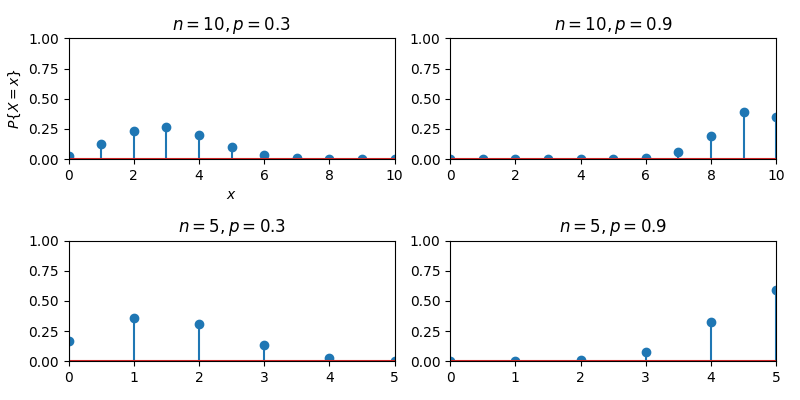
\includegraphics[height=4cm]{7.4-1.png}
\caption{二项分布}
\end{figure}

\begin{tcolorbox}
二项分布描述伯努利试验,我们可以知道在固定$n$次子试验中,事件$A$发生几次的概率是最大的。最典型的应用就是$n$次放回抽样,计算抽到$x$个次品的概率。
\end{tcolorbox}

%============================================================
\subsection{超几何分布}

{\bf 超几何分布},记作$H\left( M,N,n \right) $,因其分布律与超几何函数的级数展开式的系数类似而得名,描述不放回抽取试验,从$N$个样品中抽取$n$个,出现$x$个次品的概率分布:
\[
P\left\{ X=x \right\} =\frac{C_{N-M}^{n-x}C_{M}^{x}}{C_{N}^{n}}, \begin{array}{l}
	N>1,M\leqslant N\\
	n\leqslant N,x\in \left[ \max \left\{ 0,M+n-N \right\} ,\min \left\{ M,n \right\} \right]\\
\end{array}
\]
其中:
\begin{itemize}
    \item $N,M$:共$N$个样品,其中有$M$个次品;
    \item $n,x$:抽取$n$个,其中$x$个为次品。
\end{itemize}
超几何分布中,抽到$\frac{M}{N}\cdot n$的概率最大。

\begin{figure}[h]
\centering
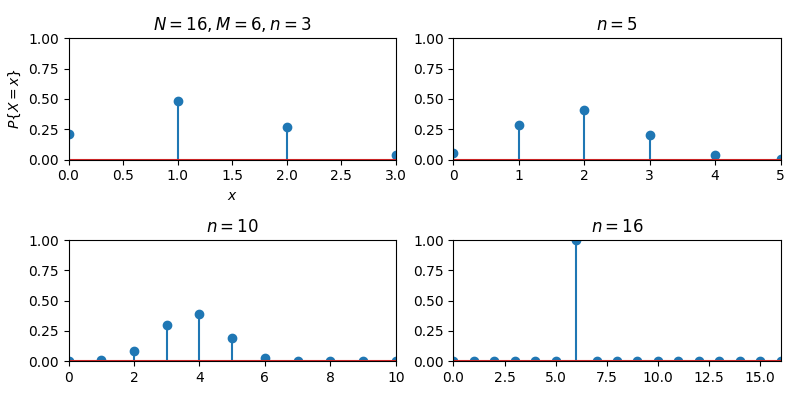
\includegraphics[height=4cm]{7.4-2.png}
\caption{超几何分布,16个样品,6个次品}
\end{figure}
\begin{figure}[h]
\centering
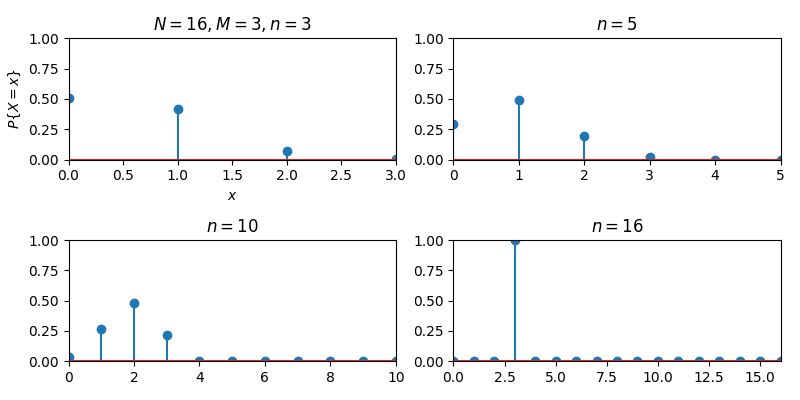
\includegraphics[height=4cm]{7.4-3.png}
\caption{超几何分布,16个样品,3个次品}
\end{figure}

\begin{tcolorbox}
超几何分布描述“不放回”抽取试验,不是基于伯努利试验,描述抽到$x$个次品的概率分布。
\end{tcolorbox}

%============================================================
\subsection{习题}

\begin{example}[综合运用7,难度:$\star $]
一个车间有3台车床,它们各自独立工作。设在一段时间内发生故障的车床数为$X$,在下列两种情形下分别求$X$的分布列。
\begin{enumerate}
    \item 假设这3台车床型号相同,它们发生故障的概率都是20\%;
    \item 这3台车床中有A型号2台,B型号1台,A型车床发生故障的概率为10\%,B型车床发生故障的概率为20\%。
\end{enumerate}
\end{example}

解:

(1)典型的二项分布:
\begin{align*}
&P\left\{ X=0 \right\} =C_{3}^{0}\cdot 0.2^0\cdot \left( 1-0.2 \right) ^{3-0}=0.512 \\
&P\left\{ X=1 \right\} =C_{3}^{1}\cdot 0.2^1\cdot \left( 1-0.2 \right) ^{3-1}=0.384 \\
&P\left\{ X=2 \right\} =C_{3}^{2}\cdot 0.2^2\cdot \left( 1-0.2 \right) ^{3-2}=0.096 \\
&P\left\{ X=3 \right\} =C_{3}^{3}\cdot 0.2^3\cdot \left( 1-0.2 \right) ^{3-3}=0.008
\end{align*}

(2)不是二项分布,需要分别计算:
\begin{align*}
P\left\{ X=0 \right\} &=\left( 1-0.1 \right) \cdot \left( 1-0.1 \right) \cdot \left( 1-0.2 \right) =0.648 \\
P\left\{ X=1 \right\} &=0.1\cdot \left( 1-0.1 \right) \cdot \left( 1-0.2 \right) \\
&+\left( 1-0.1 \right) \cdot 0.1\cdot \left( 1-0.2 \right) +\left( 1-0.1 \right) \cdot \left( 1-0.1 \right) \cdot 0.2=0.306 \\
P\left\{ X=2 \right\} &=0.1\cdot 0.1\cdot \left( 1-0.2 \right) +0.1\cdot \left( 1-0.1 \right) \cdot 0.2+\left( 1-0.1 \right) \cdot 0.1\cdot 0.2 \\
&=0.044 \\
P\left\{ X=3 \right\} &=0.1\cdot 0.1\cdot 0.2=0.002
\end{align*}

\begin{tcolorbox}
本题考察二项分布的概念,没有难度。
\end{tcolorbox}

~

\begin{example}[拓广探索8,难度:$\star \star \star $]
某药厂研制一种新药,宣称对治疗某种疾病的有效率为90\%,随机选择了10名患者,经过使用该药治疗后,治愈的人数不超过6人,你是否怀疑药厂的宣传?
\end{example}

解:

假设新药的有效率90\%为真,则治愈人数不超过6人的概率:
\begin{align*}
&P\left\{ X=0 \right\} =C_{10}^{0}\cdot 0.9^0\cdot \left( 1-0.9 \right) ^{10-0}=1\times 10^{-10} \\
&P\left\{ X=1 \right\} =C_{10}^{1}\cdot 0.9^1\cdot \left( 1-0.9 \right) ^{10-1}=9\times 10^{-9} \\
&P\left\{ X=2 \right\} =C_{10}^{2}\cdot 0.9^2\cdot \left( 1-0.9 \right) ^{10-2}=3.645\times 10^{-7} \\
&P\left\{ X=3 \right\} =C_{10}^{3}\cdot 0.9^3\cdot \left( 1-0.9 \right) ^{10-3}=8.748\times 10^{-6} \\
&P\left\{ X=4 \right\} =C_{10}^{4}\cdot 0.9^4\cdot \left( 1-0.9 \right) ^{10-4}=0.000137781 \\
&P\left\{ X=5 \right\} =C_{10}^{5}\cdot 0.9^5\cdot \left( 1-0.9 \right) ^{10-5}=0.00148803 \\
&P\left\{ X=6 \right\} =C_{10}^{6}\cdot 0.9^6\cdot \left( 1-0.9 \right) ^{10-6}=0.0111603 \\
&\sum_{i=0}^6{P\left\{ X=i \right\}}=0.0127952
\end{align*}
也即在有效率90\%的情况下治愈人数不超过6人的概率仅为仅为1.28\%,显然这个有效率90\%是小概率事件,有理由怀疑宣传的真实性。

\begin{tcolorbox}
本题是数理统计的检验假设问题,稍微有点超纲。
\end{tcolorbox}






\newpage
\section{正态分布}

~

{\bf 正态分布},也称{\bf 高斯分布},记作$N\left( \mu ,\sigma ^2 \right) $,类似泊松分布,描述一个范围内的分布情况:
\[
f\left( x \right) =\frac{1}{\sqrt{2\pi}\sigma}e^{-\frac{\left( x-\mu \right) ^2}{2\sigma ^2}},\qquad \mu \in \mathbb{R} ,\sigma >0
\]
其中:
\begin{itemize}
    \item $\mu $:数学期望,规定了中心点的横坐标,$f\left( x \right) $以$x=\mu $为对称,并在$x=\mu $取得最大值$\frac{1}{\sqrt{2\pi}\sigma}$;
    \item $\sigma $:标准差,一方面规定了$f\left( x \right) $的两个拐点$\mu \pm \sigma $,另一方面也规定了平坦度,$\sigma $越大,曲线越平坦。
\end{itemize}
特别地,当$\mu =0,\sigma =1$时,称为{\bf 标准正态分布},记作$N\left( 0,1 \right) $,此时密度函数和分布函数通常记为$\varphi \left( x \right) ,\varPhi \left( x \right) $,有:
\[
\varphi \left( x \right) =\frac{1}{\sqrt{2\pi}}e^{-\frac{x^2}{2}}\qquad \varPhi \left( x \right) =\int_{-\infty}^x{\varphi \left( t \right) \cdot dt}
\]
根据密度函数的偶函数定理,有性质:
\begin{align*}
&\varPhi \left( x \right) +\varPhi \left( -x \right) =1 \\
&\varPhi \left( 0 \right) =0.5
\end{align*}

\begin{figure}[h]
\centering
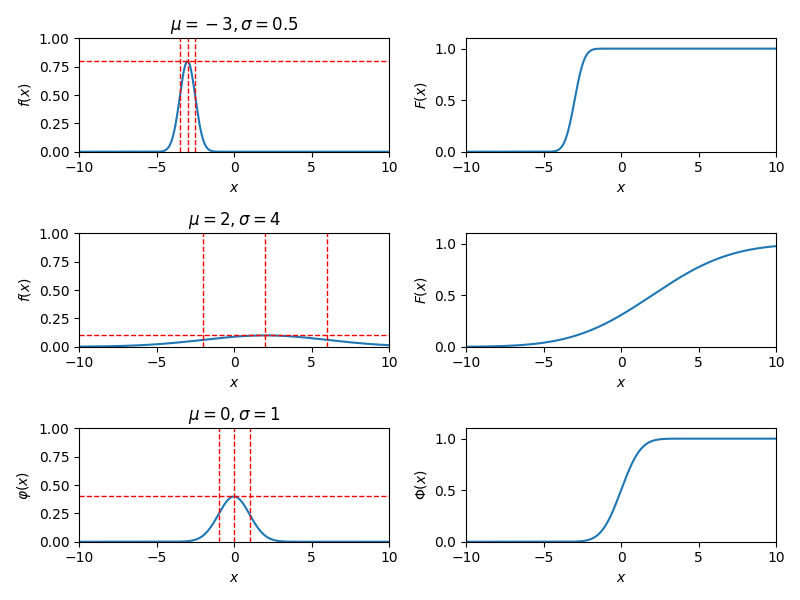
\includegraphics[height=7.5cm]{7.5-1.png}
\end{figure}

\begin{tcolorbox}
正态分布常用于描述身高、体重、成绩、元器件指标等的离散程度。
\end{tcolorbox}

\begin{theorem}
若$X\sim N\left( \mu ,\sigma ^2 \right) $,则有:
\[
P\left\{ a<X\leqslant b \right\} =\varPhi \left( \frac{b-\mu}{\sigma} \right) -\varPhi \left( \frac{a-\mu}{\sigma} \right)
\]
\end{theorem}

可用积分变量替换进行证明,略。该定理使得我们可以用标准分布计算任何正态分布。

\begin{theorem}
设$X_1\sim N\left( \mu _1,{\sigma _1}^2 \right) ,X_2\sim N\left( \mu _2,{\sigma _2}^2 \right) $ ,则$Y=X_1+X_2$也服从正态分布,且有:
\begin{align*}
&Y\sim N\left( \mu _1+\mu _2,{\sigma _1}^2+{\sigma _2}^2 \right) \\
&f\left( y \right) =\frac{1}{\sqrt{2\pi \left( {\sigma _1}^2+{\sigma _2}^2 \right)}}e^{-\frac{\left[ y-\left( \mu _1+\mu _2 \right) \right] ^2}{2\left( {\sigma _1}^2+{\sigma _2}^2 \right)}}
\end{align*}
反之,若正态分布$Y$能表示成两个变量的和$Y=X_1+X_2$,则$X_1,X_2$也必然是正态分布,这点被称为正态分布的{\bf 再生性}。
\end{theorem}

\begin{tcolorbox}
正态分布有很多特别的表现。一方面,若足够多的独立分布叠加,则总体可看成正态分布;另一方面,在相同方差的情况下,正态分布具有最大的不确定性。所以正态分布不但非常常见,而且也是优先考虑使用的模型。
\end{tcolorbox}

%============================================================
\subsection{习题}

\begin{example}[综合运用4,难度:$\star $]
袋装食盐标准质量为400g,规定误差的绝对值不超过4g就认为合格。假设误差服从正态分布,随机抽取100袋食盐,误差的样本均值为0,样本方差为4。请你估计这批袋装食盐的合格率。
\end{example}

解:

设每袋食盐的质量为随机变量$X$,则$X~N\left( 0,4^2 \right) $,误差的绝对值不超过4g就认为合格,于是食盐质量在$\pm 4$内的概率为:
\[
P\left\{ X\in \left[ -4,4 \right] \right\} =P\left\{ X\in \left[ -\sigma ,\sigma \right] \right\} =0.6827
\]
后略。

\begin{tcolorbox}
本题考察正态分布的概念,没有难度。
\end{tcolorbox}






\newpage
\section{本章小结}

本章介绍了随机变量和分布。我们将事件和概率进行数学上的抽象,上升为函数,用函数刻画概率,描绘生活中常见的概率的分布规律。

常见分布如下。
\begin{table}[h]
\centering
\begin{tabular}{ll}
    \toprule
    \multicolumn{1}{c}{分布} & \multicolumn{1}{c}{含义、用途}  \\
    \midrule
    二项分布$B\left( n,p \right) $ & $n$重伯努利试验中发生$x$次的概率分布。\\
    超几何分布$H\left( M,N,n \right) $ & 不放回抽取中,抽到含$x$个次品的概率分布。\\
    正态分布$N\left( \mu ,\sigma ^2 \right) $ & 描述某指标的离散度。\\
    \bottomrule
\end{tabular}
\end{table}

此外还有几何分布、均匀分布、指数分布等,略。

%============================================================
\subsection{习题}

\begin{example}[复习巩固3,难度:$\star $]
假设有两箱零件,第一箱内装有10件,其中有2件次品;第二项内装有20件,其中有3件次品。现从两箱中随意挑选一箱,然后从该箱中随机取1个零件。
\begin{enumerate}
    \item 求取出的零件是次品的概率;
    \item 已知取出的是次品,求它是从第一箱取出的概率。
\end{enumerate}
\end{example}

解:

(1)全概率问题,易得:
\[
P\left( A \right) =0.5\cdot \frac{2}{10}+0.5\cdot \frac{3}{20}=0.175
\]

(2)
\[
P\left( B \middle| A \right) =\frac{P\left( BA \right)}{P\left( A \right)}=\frac{0.5\cdot \frac{2}{10}}{0.175}=0.571429
\]

\begin{tcolorbox}
本题考察全概率公式和条件概率,没有难度。
\end{tcolorbox}

~

\begin{example}[复习巩固5,难度:$\star \star $]
已知随机变量$X$取所有的值$1,2,\cdots ,n$是等可能的,且$E\left( X \right) =10$,求$n$的值。
\end{example}

解:
\begin{align*}
E\left( X \right) &=1\cdot \frac{1}{n}+2\cdot \frac{1}{n}+\cdots +n\cdot \frac{1}{n} \\
&=\frac{1}{n}\cdot \sum_{i=1}^n{i}=\frac{1}{n}\cdot \frac{n\left( 1+n \right)}{2}=\frac{1+n}{2}=10
\end{align*}
得$n=19$。

\begin{tcolorbox}
本题结合了数列的知识。
\end{tcolorbox}

~

\begin{example}[复习巩固6,难度:$\star $]
已知每门大炮击中目标的概率都是0.3,现在$n$门大炮同时对某一目标各射击一次。
\begin{enumerate}
    \item 当$n=10$时,求恰好击中目标3次的概率(精确到0.001);
    \item 如果使目标至少被击中一次的概率超过95\%,至少需要多少门大炮?
\end{enumerate}
\end{example}

解:

(1)是典型的二项分布,易得:
\[
P\left\{ X=3 \right\} =C_{10}^{3}\cdot 0.3^3\cdot \left( 1-0.3 \right) ^{10-3}=0.266828
\]

(2)题目也即没有击中的概率小于5\%,有:
\begin{align*}
&\because P\left\{ X=0 \right\} =C_{n}^{0}\cdot 0.3^0\cdot \left( 1-0.3 \right) ^{n-0}<0.05 \\
&\therefore 1\cdot 1\cdot 0.7^n<0.05 \\
&\therefore n>\log _{0.7}0.05=\frac{\ln 0.05}{\ln 0.7}=8.39905
\end{align*}
至少需要9门。

\begin{tcolorbox}
本题(2)转换成不击中能极大减小计算量。
\end{tcolorbox}

~

\begin{example}[综合运用9,难度:$\star $]
假设一份某种意外伤害保险费为20元,每次赔付金额为50万元。一家保险公司一年能销售10万份保单,而每一份保单需要赔付的概率为$10^{-5}$。利用计算工具求(精确到0.0001):
\begin{enumerate}
    \item 这家保险公司在这个险种上亏本的概率;
    \item 这家保险公司在这个险种上一年内获利不少于100万元的概率?
\end{enumerate}
\end{example}

解:

本题为典型的二项分布问题。

(1)易得收益$20\cdot 100000=2000000$,也即出现4次以上(不包含4次)赔付就亏本,于是:
\begin{align*}
&P\left\{ X=0 \right\} =C_{100000}^{0}\cdot \left( 10^{-5} \right) ^0\cdot \left( 1-10^{-5} \right) ^{100000-0}=0.367878 \\
&P\left\{ X=1 \right\} =C_{100000}^{1}\cdot \left( 10^{-5} \right) ^1\cdot \left( 1-10^{-5} \right) ^{100000-1}=0.367881 \\
&P\left\{ X=2 \right\} =C_{100000}^{2}\cdot \left( 10^{-5} \right) ^2\cdot \left( 1-10^{-5} \right) ^{100000-2}=0.183941 \\
&P\left\{ X=3 \right\} =C_{100000}^{3}\cdot \left( 10^{-5} \right) ^3\cdot \left( 1-10^{-5} \right) ^{100000-3}=0.0613129 \\
&P\left\{ X=4 \right\} =C_{100000}^{4}\cdot \left( 10^{-5} \right) ^4\cdot \left( 1-10^{-5} \right) ^{100000-4}=0.0153279 \\
&1-\sum_{i=0}^4{P\left\{ X=i \right\}}=1-0.99634=0.00365962
\end{align*}
亏本的概率为0.366\%。

(2)即赔付0、1次的概率:
\[
\sum_{i=0}^1{P\left\{ X=i \right\}}=0.367878+0.367881=0.735759
\]

\begin{tcolorbox}
本题考察二项分布的概念。
\end{tcolorbox}

~

\begin{example}[拓广探索10,难度:$\star \star \star \star $]
甲、乙、丙三人相互做传球训练,第1次由甲将球传出,每次传球时,传球者都等可能地将球传给另外两个人中的任何一人。
求$n$次传球后球在甲手中的概率。
\end{example}

解:

即求$P\left\{ X=n \right\} $的表达式,假设我们知道这个表达式了,则$n+1$次后球在甲手中的概率:
\[
P\left\{ X=n+1 \right\} =\frac{1-P\left\{ X=n \right\}}{2}\cdot \frac{1}{2}\cdot 2=\frac{1-P\left\{ X=n \right\}}{2}
\]
其中,$1-P\left\{ X=n \right\} /2$表示乙丙两人每人得球概率,除以2表示他们各自都有一半的可能传给甲,再乘以2表示两人一共传给甲的概率。
稍作化简:
\begin{align*}
&P\left\{ X=n+1 \right\} +C=-\frac{1}{2}\cdot \left( P\left\{ X=n \right\} -2C-1 \right) \\
&C=-2C-1 \\
&C=-\frac{1}{3} \\
&P\left\{ X=n+1 \right\} -\frac{1}{3}=-\frac{1}{2}\cdot \left( P\left\{ X=n \right\} -\frac{1}{3} \right)
\end{align*}
可见$P\left\{ X=n \right\} -1/3$是一个等比数列,于是:
\begin{align*}
&\because P\left\{ X=1 \right\} -\frac{1}{3}=0-\frac{1}{3}=-\frac{1}{3} \\
&\therefore P\left\{ X=n \right\} -\frac{1}{3}=\left( -\frac{1}{3} \right) \cdot \left( -\frac{1}{2} \right) ^{n-1} \\
&\therefore P\left\{ X=n \right\} =\left( -\frac{1}{3} \right) \cdot \left( -\frac{1}{2} \right) ^{n-1}+\frac{1}{3}
\end{align*}

\begin{tcolorbox}
本题是马尔科夫链,略有超纲,但结合数列的知识还是能解。
\end{tcolorbox}

~

\begin{example}[拓广探索11,难度:$\star \star $]
某单位有10000名职工,想通过验血的方法筛查乙肝病毒携带者。假设每人携带乙肝病毒的概率为5\%,如果对每人的血样逐一化验,就需要化验10000次。统计专家提出了一种化验方法:随机地按5人一组分组,然后将各组5人的血样混合再化验。如果混合血样呈阴性,说明这5人全部阴性;如果混合血样呈阳性,说明其中至少有一人的血样呈阳性,就需要对每人再分别化验一次。
\begin{enumerate}
    \item 按照这种化验方法能减少化验次数吗?
    \item 如果每人携带乙肝病毒的概率为2\%,按照$k$人一组,$k$取多大时化验次数最少?
\end{enumerate}
\end{example}

解:

(1)可以通过考察数学期望判断化验次数。易得单位有500名携带者,于是5人一组存在阳性的概率:
\[
1-P\left\{ X=0 \right\} =1-0.95^5=0.226219
\]
化验次数:
\[
\frac{10000}{5}+5\cdot 0.226219=2001.13
\]
可见确实能减少次数。

(2)概率为2\%时,有200人携带,于是$k$人一组的化验次数:
\begin{align*}
&P\left( k \right) =1-P\left\{ X=0 \right\} =1-0.98^k \\
&f\left( k \right) =\frac{10000}{k}+P\left( k \right) \cdot k=\frac{10000}{k}+k-0.98^k\cdot k
\end{align*}
即求函数$f\left( k \right) $的最值,求导即可,有点复杂,略。
\[
f'\left( x \right) =\frac{-10000}{k^2}+1-0.98^k\left( \ln 0.98\cdot k+1 \right)
\]

\begin{tcolorbox}
本题关键捋清分组的过程。
\end{tcolorbox}










\chapter{成对数据的统计分析}

本章粗略介绍数理统计的相关知识。

本章要点:
\begin{itemize}
    \item 相关性。
    \item 线性回归。
    \item 独立性。
\end{itemize}

\newpage
\section{成对数据的统计相关性}

详细了解相关性需要微积分和线性代数的知识,高中课本只是粗略介绍,XML。可详见我的《概率论与数理统计——学习笔记》。

值得一提的是P98将相关和向量类比,反复阅读体会。






\newpage
\section{一元线性回归模型及其应用}

详细了解相关性需要微积分和线性代数的知识,高中课本只是粗略介绍,XML。可详见我的《概率论与数理统计——学习笔记》。






\newpage
\section{列联表与独立性检验}

详细了解相关性需要微积分和线性代数的知识,高中课本只是粗略介绍,XML。可详见我的《概率论与数理统计——学习笔记》。






\newpage
\section{扩展知识:概率论和数理统计的知识结构}

概率论和数理统计这门学科,国外分为两本教材,分别是“概率论”和“数理统计”,国内作为理工科入门教材一般都合在一本。学科分为两部分,概率论和数理统计,前者是后者的理论基础,后者是前者的工程应用。

概率论一般分4大部分:
\begin{itemize}
    \item 随机事件:主要介绍概率的相关知识,如条件概率、全概率、贝叶斯公式、古典概型、几何概型等;
    \item 随机变量:将随机事件抽象,用函数这一工具讨论概率,主要讲随机变量的分布,如二项分布、泊松分布、正态分布等,若干个随机变量的关系,如边缘分布、条件分布、独立性等;
    \item 数字特征:讲述数学期望、方差、协方差、相关系数、矩等;
    \item 大数定理和中心极限定理:作为概率论的补完。
\end{itemize}

数理统计一般分3大部分:
\begin{itemize}
    \item 基础:主要介绍基本概念,如总体、样本、抽样;
    \item 参数估计:讲述如何用样本估计总体的参数,如估计总体的期望、方差等,以及对估计方法的评价;
    \item 假设检验:对总体的一些假设,我们如何用已知的样本进行对这个假设的判断,或者说我们如何用数学的方法定量地判断一个假设的可信度。
\end{itemize}

可见,高中选修教材第三册中,除了本章第三节是属于数理统计的假设检验部分,其他都是概率论部分的内容。概率论和数理统计虽然视作数学,但其实是建立在微积分和线性代数的基础上。若缺乏这两个基础,所有知识点都不可能进行有效深入地讨论。






\newpage
\section{本章小结}

本章介绍了两个随机变量的相关概念——相关性,线性回归拟合,独立性检验。












\end{document}




